\chapter{Photon Detection System}
\label{ch:fddp-pd}

%%%%%%%%%%%%%%%%%%%%%%%%%%%%%%%%%%%%%%%%%%%%%%%%%%%%%%%%%%%%%%%%%%%%
\section{Overview}
\label{sec:fddp-pd-1}

%%%%%%%%%%%%%%%%%%%%%%%%%%%%%%%%%
\subsection{Introduction}
\label{sec:fddp-pd-1.1}

This chapter describes the \dword{pds} for the \dword{dpmod}. The \dword{pds} is used primarily as decision to acquire the event (trigger) for non-beam events, for determination of the event absolute time for beam and non-beam events, and for calorimetric measurements. It is essential to ensure that the \dual \dword{pds} is optimized for the full DUNE physics program. In particular, low-energy signals like \dword{snb} neutrinos and multi-messenger astronomy, other low-energy signals, and proton decay, will have more stringent requirements on \dword{pds} performance than the primarily higher energy, beam-synchronous, neutrino oscillation physics. The final specifications of the system will be determined in order to achieve these physics requirements. See \voltitlespfd{}, Chapter 6.

This %Technical Proposal
 chapter concentrates on direct projection of the \dword{pddp} design to the DUNE scale. The optimization and final design of the \dual \dword{pds} is driven by the \dword{pddp} \cite{protoDUNDP-tdr} data and simulation studies.

The chapter begins with an overview of the system in Section~\ref{sec:fddp-pd-1}. Section~\ref{sec:fddp-pd-2} describes the photosensors, namely \dwords{pmt} %tubes  
and the related \dword{hv} system, wavelength shifters and light collectors. The mechanics associated with the \dwords{pmt} is described in Section~\ref{sec:fddp-pd-3}, and the readout electronics in~\ref{sec:fddp-pd-4}. Section~\ref{sec:fddp-pd-5} details the photon calibration system to monitor the \dword{pmt} gain and stability. Then, the \dword{pd} performance is described in Section~\ref{sec:fddp-pd-6}, and the operations in Section~\ref{sec:fddp-pd-7}. Interfaces with other subsystems are described in Section~\ref{sec:fddp-pd-8}. Section~\ref{sec:fddp-pd-9} includes the installation, integration and commissioning plans. The \dword{qc} procedures are outlined in Section~\ref{sec:fddp-pd-10}. The main safety issues to consider are specified in Section~\ref{sec:fddp-pd-11}. To finish, the management and organization is described in Section~\ref{sec:fddp-pd-12}.

%%%%%%%%%%%%%%%%%%%%%%%%%%%%%%%%%
\subsection{Physics and the Role of Photodetection}
\label{sec:fddp-pd-1.2}

The main physics goals of the \dword{dpmod} is to register beam events %from LBNF at \fnal, 
and operate outside of the beam spill as an efficient observatory for \dwords{snb} and proton decays. DUNE will also collect atmospheric neutrino and muon events, and will conduct searches for a number of exotic phenomena postulated by extensions of the Standard Model.  Expected or searched for signals can range in energy from a few \si{MeV} to many \si{GeV} and have characteristic time duration and topological features that challenge the performance of large noble liquid TPCs. An essential and critical part of the \lartpc is the \dword{pds}, sensitive to light produced by interactions in argon \cite{Cuesta:2017nrs}. In DP TPCs, the timing of prompt scintillation light (usually referred as S1 signal) in \lar is needed for time stamping of events and propagation of tracks in the detector. The extraction and amplification of drift electrons in the gas phase (usually referred to as S2 signal) yields information on the drift time and amount of ionization charge, thus supplementing information from the charge readout on the anode plane. The interplay between the charge and light from an event allows to achieve the pattern recognition and the measurement of energy of interactions.

Ionizing radiation in liquid noble gases leads to the formation of excimers in either singlet or triplet states, which decay radiatively to the dissociative ground state with characteristic S1 fast and slow lifetimes (fast is about \SI{6}{ns}, slow is about \SI{1.3}{$\mu$s} in \lar with the so-called second continuum emission spectrum peaked at the wavelength of approximately \SI{127}{nm}, \SI{126.8}{nm} with a full width at half maximum of \SI{7.8}{nm} \cite{Heindl}). This prompt and relatively high-yield (about \num{40000} photons per \si{MeV}) of \SI{127}{nm} scintillation light is exploited in \lartpc to provide the absolute time ($t_0$) of the ionization signal collected at the anode, thereby providing the absolute value of the drift coordinate of fully contained events, as well as a prompt signal used for triggering purposes.

The secondary scintillation light S2 is produced in the gas phase of the \dword{dpmod} when electrons, extracted form the liquid, are accelerated in the \efield between the liquid phase and the anode. The secondary scintillation in the argon gas (i.e., a vapor phase) is the luminescence in gas caused by accelerated electrons in the \efield and in the \dword{lem} anode through Townsend amplification. For a given argon gas density, the number of photons of this S2 signal is proportional to the number of electrons, the \efield, and the length of the drift path in gas covered by the electrons. In an extraction field of \SI{2.5}{kV/cm} in gas, one electron generates about \num{75} photons. The time stretch of S2 reflects the extraction time of original ionization in the liquid phase into the gas phase, thus for about \SI{1}{kV/cm} \efield, the time scale of S2 is of the order of hundreds of microseconds. The time between the occurrence of the primary scintillation light and the secondary scintillation light is equivalent to the drift time of the electrons from the ionization coordinate to the \lar surface.

The baseline design of the light collection system calls for \SI{20.3}{cm} (\SI{8}{in}) diameter cryogenic \dwords{pmt} distributed uniformly on the floor of the cryostat and electrically shielded from the bottom cathode plane. The proposed density of \dwords{pmt} and their arrangement follows the design of the \dword{pddp} detector. On the other hand, modeling and simulations of light collection both for \dword{pddp} and the DUNE \dwords{detmodule} are still ongoing. Therefore, even critical system parameters and their impact on the physics reach are still tentative. Results from the \dword{pddp} will provide the critical validation of simulations and will guide optimizations for the large \dword{dpmod}.

%%%%%%%%%%%%%%%%%%%%%%%%%%%%%%%%%
\subsection{Technical Requirements}
\label{sec:fddp-pd-1.3}

\Dwords{pmt} provide the sharpest time information of events in the \lartpc and in the gas phase of the extraction stage. Due to necessary wavelength-shifting of photons from the argon luminescence and shadowing by the cathode plane, the efficiency of light detection is challenging and requires careful mechanical, electrical, and optical designs. The \dual \dword{pd} consortium is presently in contact with \dword{pmt} manufacturers, including 
%
Hamamatsu Photonics~\footnote{Hamamatsu Photonics\texttrademark{}, \url{http://www.hamamatsu.com/resources/pdf/etd/LARGE_AREA_PMT_TPMH1286E.pdf}} in Japan %~ 
% \cite{hamamatsu}, 
Electron Tubes Limited~\footnote{Electron Tubes Ltd\texttrademark{}, \url{http://www.electron-tubes.co.uk//}} in the USA and UK, and 
% ~\cite{electrontubeslim}
HZC~\footnote{HZC Photonics\texttrademark{}, \url{http://hzcphotonics.com/en_index.html}.} in China, 
% \cite{hzc}
to define optimal choice and configuration of \dwords{pmt} satisfying our requirements, tentatively summarized in Table~\ref{tab:dppd_t_1_3}. These requirements will be reviewed based on the physics needs. For this, simulations and \dword{pddp} results will be key.

\begin{dunetable}
[Summary of tentative requirements for the \dword{dpmod} \dword{pds}] % photon detection system of the DP \lartpc.]
%{|l|l|l| p{0.8\textwidth}}
{p{0.25\textwidth} p{0.3\textwidth} p{0.45\textwidth}}
{tab:dppd_t_1_3}
{Summary of tentative requirements for the \dword{dpmod} \dword{pds} %the \dword{pds} of the DP \lartpc. 
The table assumes the baseline choice of the R5912-MOD20 \dword{pmt} manufactured by Hamamatsu Photonics \cite{hamamatsu-5912}.}
\footnotesize
%  & & \\
{\bf Feature}	& {\bf Goal}  	& {\bf Comment	}	\\
%  & & \\ 
 \toprowrule
{\bf Optical} & & \\ \colhline
spectral response & \SI{127}{nm} 	& wavelength shifters are required				\\
light yield & 2.5 \phel/\si{MeV} & for \dword{pddp}, final value depending on \\

 	 & 	 & simulation results \\
\colhline
{\bf Electronic}	&			&										\\ \colhline
minimum light signal & SPE & required to perform the \dword{pmt} gain measurement \\
gain			& $\sim$\num{e6}-\num{e9} & given by \dword{pmt} specifications			\\
noise (or signal/noise) &  <\SI{1}{mV} & to distinguish SPE from noise, depends on \dword{pmt} gain
\\
timing resolution & few ns & to distinguish S1 from S2 component \\
	power		& < \SI{0.2}{W/\dword{pmt}}& used successfully in the  \dword{wa105} $3\times1\times1$\,m$^3$ detector			\\
\dword{adc} dynamic range & TBD & depending on simulation results, see section \ref{sec:fddp-pd-4.3}  \\ 
\colhline		
 	{\bf Electrical}	&			&									\\ \colhline
 	\dword{hv} range		& \si{0-2500}{V}	& individual cable per each \dword{pmt}			\\
	\dword{hv} resolution	& \SI{1}{V}		&	fine tuning of \dword{pmt} gain			\\
	\dword{hv} noise		& <\SI{100}{mV}		& extra filtering will be required \\
	\dword{hv} grounding	& isolated		& \dword{hv} outputs shall be floating, crate ground is 	\\
				&			& independent of the return of the \dword{hv} channels. 			\\ 
\dword{pmt} placement		& isolated		& \dword{pmt}'s electrically shielded from the TPC cage	\\
\colhline			
      {\bf Mechanical} 	&			&									\\ \hline
      	temperature 	& cryogenic		& \dwords{pmt} operated in \lar and tested in liquid nitrogen 	\\
	pressure 		& \SI{+2}{bar}		& the argon column will be about \SI{10}{m} high	\\		
\end{dunetable}

\Dwords{pmt} will be installed with the baseline density of \num{1} per \SI{1}{m^2}. The choice of the Hamamatsu R5912-MOD20 \dword{pmt} %manufactured by Hamamatsu Photonics \cite{hamamatsu-5912} 
is assumed as baseline plan. In order to extend the \dword{pmt} light sensitivity region to the \lar light emission wavelength of \SI{127}{nm}, a wavelength shifter has to be used. Therefore, in the baseline plan, the hemispherical windows of the \dwords{pmt} are evaporated with a thin layer of \dword{tpb}~\cite{tpb} for wavelength-shifting into the range suitable for R5912 \dword{pmt} photocathode sensitivity~\cite{hamamatsu-5912}. \Dwords{pmt} have to be rigidly anchored to the bottom of the cryostat. Different \dword{pmt} densities and placements along the walls are also being considered in simulations. \dword{hv} signal cables are routed along the cryostat walls to \fdth{}s installed in the roof of the cryostat. Each \dword{pmt} is controlled individually so that its gain can be individually adjusted to match the \dword{fe} dynamic range and \dword{s/n} ratio. An average light yield of \SI{2.5}{\phel/MeV} is required based on \dword{pddp} simulations (see Section~\ref{sec:fddp-pd-6}). The precision of the light yield requirement will be established after the completion of the full DUNE simulations.

The cathode plane, described in Chapter~\ref{ch:fddp-hv}, %the \dword{hv} chapter, 
 is placed at a height of about \SI{2}{m} above the bottom of the cryostat, and the \dword{pmt} plane is distant enough from the cathode plane, taking into account the high electrical rigidity of the \lar phase. In order to protect the \dwords{pmt}, the ground grid is installed and placed at an identical potential as the \dword{pmt} photocathode (\SI{0}{V}). The \dwords{pmt} are powered to about \numrange{1.5}{2.0}\si{kV} such that the \dword{pmt} gain is $\sim$\numrange{e7}{e9}. Future developments on the quantization of possible \dword{tpb} dissolution in \lar will be encouraged and followed \cite{TPBdiss}.

%%%%%%%%%%%%%%%%%%%%%%%%%%%%%%%%%
\subsection{Detector Layout}
\label{sec:fddp-pd-1.4}

The \dword{pmt} plane is placed far enough below the cathode plane to be sufficiently electrically shielded. According to the baseline plan, the \dwords{pmt} is uniformly distributed across this plane with a density of \SI{1}{\dword{pmt}/m^2}, with a total of \dpnumpmtch \dwords{pmt} installed. Other \dword{pmt} configurations as determined by the simulations are also being considered. The \dwords{pmt} are individually mounted to the cryostat floor. The exact location of the \dwords{pmt} will be determined by the location of the other floor structures like the cryogenic piping. The outline of the \dword{dpmod} is shown in Figure~\ref{fig:dppd_3_1}.

\begin{dunefigure}[The \dword{dpmod} (partially open)]{fig:dppd_3_1}
{The \dword{dpmod} (partially open) with cathode, \dwords{pmt}, \dword{fc} and anode plane with chimneys.}
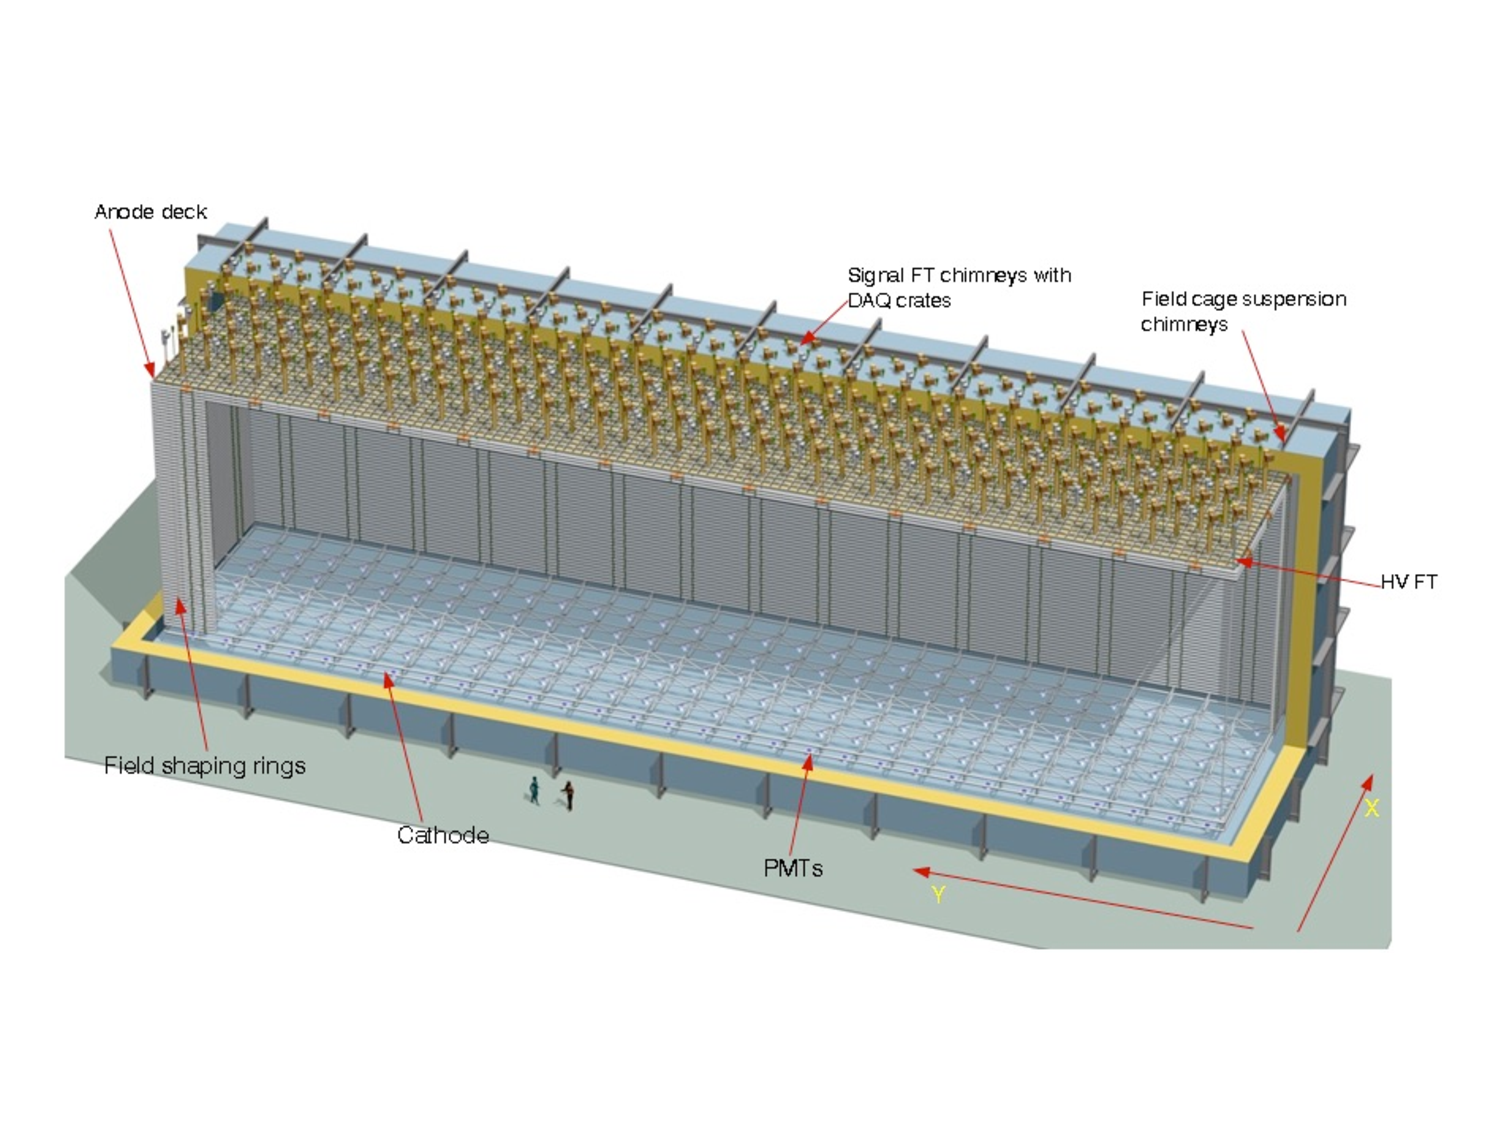
\includegraphics[width=0.95\textwidth]{dppd_3_1}
\end{dunefigure}

Since few light sensors are directly sensitive to \SI{127}{nm}, a wavelength shifter is required. \dword{tpb} coating directly on the \dword{pmt} is the default plan. Light collectors to increase the photons detected are under study. A single cable per \dword{pmt} carries power and signal, and splitters are placed out of the cryostat. A photon calibration system will be formed by external light sources and internal optical fibers.  

The cable trays from the side walls of the cryostat to the \dwords{pmt} carry the cables and calibration fibers. The cables and fibers are routed from the \fdth flanges at the top of the cryostat and  combined at the side wall trays. These side trays carry the \dword{hv}/signal cables in blocks of \num{24} \dwords{pmt} and four calibration fibers. Therefore, each block of \num{24} \dwords{pmt} in a \num{6}$\times$\SI{4}{m^2} area forms a sector of underground installation, totaling \num{30} sectors.

% %%%%%%%%%%%%%%%%%%%%%%%%%%%%%%%%%
\subsection{Operation Principles}
\label{sec:fddp-pd-1.5}

The physics program defines the operation principles of the \dword{dpmod}: the measurement of the neutrino oscillation parameters requires recording events based on an external trigger coming from the beam, while non-beam physics such as  \dwords{snb}, proton decay, or other exotic transitions events, require special trigger conditions, including the \dword{pds}. \Dword{pmt} calibration, which has to be performed regularly, presents another operation mode wherein  a hardware trigger provided by the calibration system starts the data recording. \\    

Thus, the operation modes are:
\begin{itemize}
\item External trigger: %this is mainly the case of 
the typical case is when the beam generates a hardware trigger,  %generated by the beam, 
but it also includes software-generated triggers for test data.
%also test data with random trigger generated by software can be taken. 
\item Non-beam physics trigger: the electronics based on the \dword{pds} signals provides the trigger for  \dword{snb}, proton decay events, etc.
\item Calibration: during \dword{pds} calibrations, the trigger is provided by the light calibration system.
\end{itemize}

%The modes of the external trigger and the non-beam physics trigger will not be excluding each other but will be running in parallel to ensure that rare events such as  \dwords{snb} are recorded effectively.
The external and non-beam physics triggers run in parallel to ensure that rare events such as  \dwords{snb} are recorded effectively.

%%%%%%%%%%%%%%%%%%%%%%%%%%%%%%%%%%%%%%%%%%%%%%%%%%%%%%%%%%%%%%%%%%%%
\section{Photosensor System}
\label{sec:fddp-pd-2}

%%%%%%%%%%%%%%%%%%%%%%%%%%%%%%%%%
\subsection{Photodetector Selection and Procurement}
\label{sec:fddp-pd-2.1}

The \dword{pd} %photodetector 
selected as baseline for the light-readout system is the Hamamatsu R5912-MOD20 \dword{pmt} as used in \dword{pddp}. The Hamamatsu R5912-MOD20, see Figure \ref{fig:dppd_2_1}, is an 8-inch, 14-stage, high gain \dword{pmt} (nominal gain of \num{e9}). In addition, this \dword{pmt} was designed to work at cryogenic temperature adding a thin platinum layer between the photocathode and the borosilicate glass envelope to preserve the conductance of the photocathode at low temperature. This particular \dword{pmt} has proven reliability on other cryogenic detectors. The same or similar \dwords{pmt} have been successfully operated in other \lar experiments like MicroBooNE \cite{microboone}, MiniCLEAN \cite{miniclean}, ArDM, ICARUS T600 \cite{icarus}, as well as in \dword{pddp} \cite{protoDUNDP-tdr}. Contacts with other manufacturers such as Electron Tubes Limited (UK) \cite{electrontubeslim} and HZC (China) \cite{hzc} are on-going to engage them in the program.

\begin{dunefigure}[Picture of the Hamamatsu R5912-MOD20 \dword{pmt}.]{fig:dppd_2_1}
{Picture of the Hamamatsu R5912-MOD20 \dword{pmt} \cite{hamamatsu-5912}.}
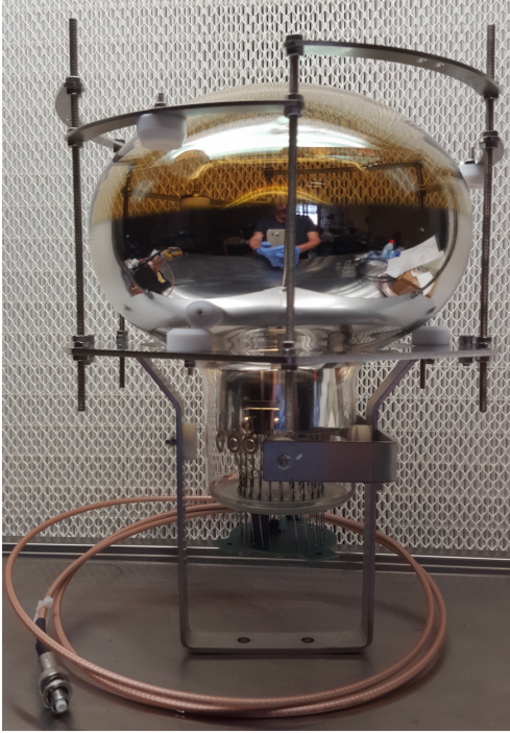
\includegraphics[width=0.2\textwidth]{dppd_2_1}
\end{dunefigure}

As the baseline number of \dwords{pmt}, \dpnumpmtch + \num{80} spares, is high and several operations and tests have to be performed with them before the installation, the \dwords{pmt} have to be ordered with sufficient time in advance to complete the following planned operations: assembly of the voltage divider circuit, mounting on the support structure, testing at room and cryogenic temperatures, application of \dword{tpb} coating, packing and shipment. They are %And finally, they have to be 
re-tested at \surf before installation (see Sections~\ref{sec:fddp-pd-9} and \ref{sec:fddp-pd-10}). Considering the large number of \dwords{pmt} required by \dual \dword{pd}, the purchase order %has to be sent, at least, 
must be completed at least two years ahead of installation. A staged or staggered order allowing us to receive a steady supply of \dwords{pmt} would be most convenient. % to execute the plan mentioned before. 

%%%%%%%%%%%%%%%%%%%%%%%%%%%%%%%%%
\subsection{Photodetector Characterization}
\label{sec:fddp-pd-2.2}

Prior to installation, the most important parameters of the \dword{pmt} response have to be measured with two aims: first, to reject under-performing \dwords{pmt} and second, to store the characterization information in a database for later use during the \dword{dpmod} commissioning and operation.

The basic and most important parameters to characterize are the dark counts rate versus voltage and the gain versus voltage. Both parameters must be measured at both room and  cryogenic temperatures. Prepulsing and afterpulsing are not expected to be an issue, but will be measured, too. 

From the mechanical point of view, the test setup requires a light-tight vessel filled with a cryogenic liquid (argon or nitrogen) plus the infrastructure for filling and operating the vessel with temperature and liquid-level controls. For \dword{pddp}, \num{10} \dwords{pmt} were tested at a time %during 
over the space of a week, as the tests of the \dwords{pmt} on cryogenics 
\fixme{as cryogenic tests of \dwords{pmt}?}
require several days for the \dword{pmt} thermalization. Figure~\ref{fig:dppd_2_2a} shows the  \dword{pddp} \dwords{pmt} being installed in the testing vessel. % used for the \dwords{pmt}. 
Increasing the capacity of the vessel, and thus the number of \dwords{pmt} to test simultaneously, %tested at a time, 
will reduce the characterization test duration.

\begin{dunefigure}[Picture of the \dwords{pmt} being installed in the testing vessel used for the \dword{pddp} \dwords{pmt}]{fig:dppd_2_2a}
{Picture of the \dwords{pmt} being installed in the testing vessel used for the \dword{pddp} \dwords{pmt}.}
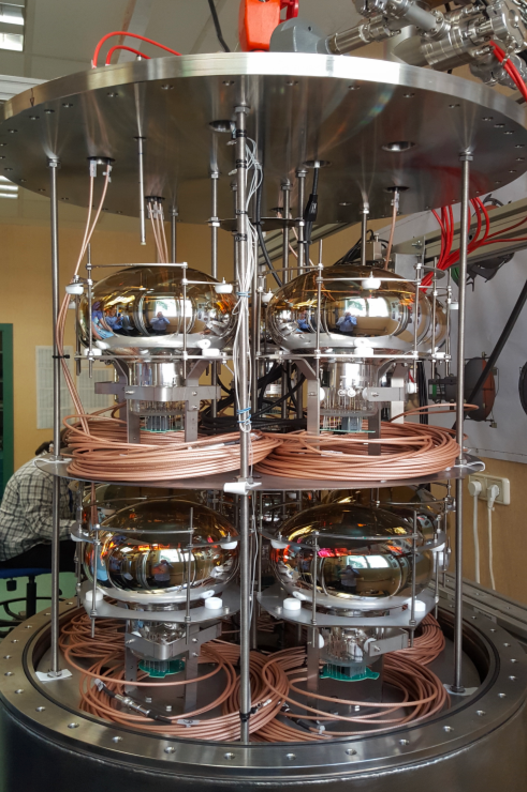
\includegraphics[width=0.3\textwidth]{dppd_2_2a}
\end{dunefigure}

Figure~\ref{fig:dppd_2_2b} shows the sketch of the envisaged setup for \dword{pmt} characterization tests. From the electronics point of view, the test setup requires a \dword{hv} power supply, a discriminator, a counter for the dark rate measurements, a pulsed light source, and a charge-to-digital or analog-to-digital converter for the \dword{pmt} gain versus voltage measurements. All those instruments must allow computer control to automate the data acquisition.

\begin{dunefigure}[Sketch of the setup for \dword{pmt} characterization tests.]{fig:dppd_2_2b}
{Sketch of the setup for \dword{pmt} characterization tests.}
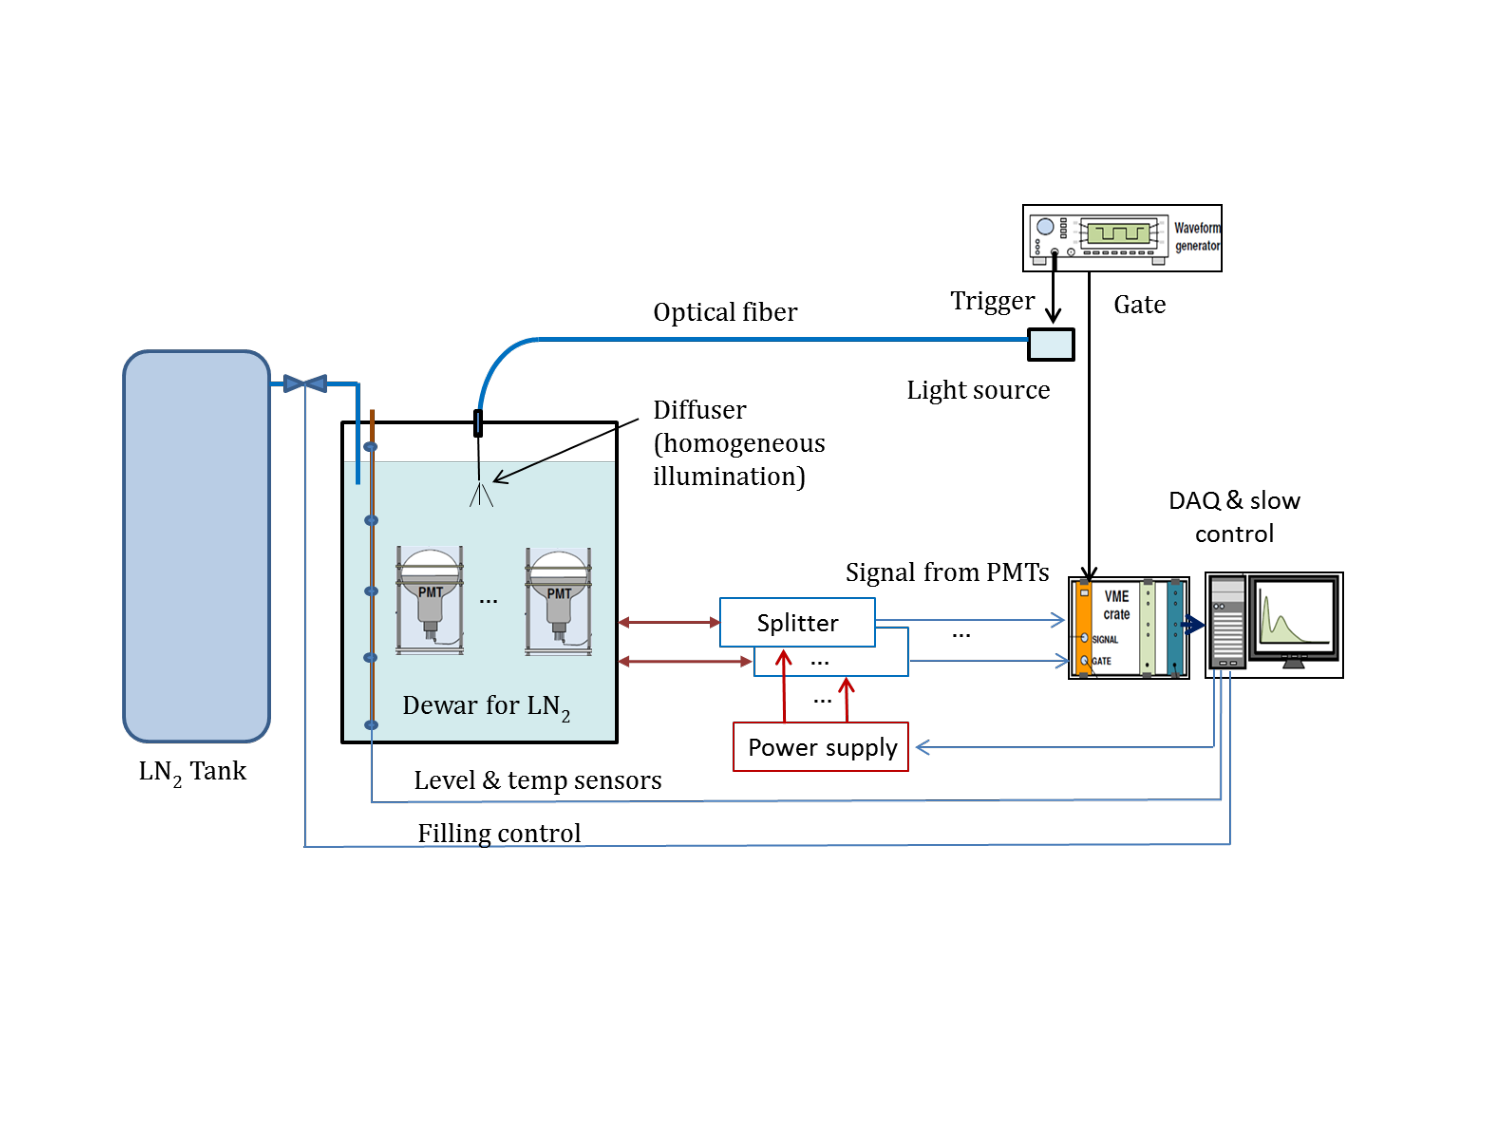
\includegraphics[width=0.9\textwidth]{dppd_2_2b}
\end{dunefigure}

%%%%%%%%%%%%%%%%%%%%%%%%%%%%%%%%%
\subsection{High Voltage System}
\label{sec:fddp-pd-2.3}

Based on the experience with the \dword{wa105} %$3\times1\times1$\,m$^3$ \dual 
prototype, %for the \dword{pmt} \dword{hv} system, the A7030 power supply modules from CAEN \cite{caen-a7030} were chosen as baseline design. 
the A7030 power supply modules from CAEN~\footnote{CAEN\texttrademark{}, \url{http://www.caen.it/csite/CaenFlyer.jsp?parent=222}} 
%\cite{caen-a7030} 
will form the baseline design of the \dword{pmt} \dword{hv} system. 
These modules provide up to \SI{3}{kV} with a maximal output current of \SI{1}{mA} and a common floating ground to minimize the noise. Module versions with \num{12}, \num{24}, \num{36}, or \num{48} \dword{hv} channels are available. The \dword{hv} polarity can be chosen for each module. According to the baseline \dword{pmt} powering scheme, modules with positive \dword{hv} polarity will be acquired for the experiment. Modules with \num{48} \dword{hv} channels and Radiall \num{52} connectors are %considered. 
under consideration. The corresponding \dword{hv} cable will connect the modules with the \dword{hv} splitters, described in Section \ref{sec:fddp-pd-4.2}. This choice will allow the design of a compact and most cost-effective system occupying only %between 
\num{1} to \num{2} racks. % only. 
For \dpnumpmtch \dwords{pmt}, \num{15} A7030 modules (+ \num{2} spares) will be needed. These \num{15} \dword{hv} modules will be installed in mainframes from CAEN.

Each \dword{pmt} is powered individually thus allowing the gain of all \dwords{pmt} to be equalized by adjusting the operating voltage. %A control software for this task will be provided taking into account the development of an interface to the \dword{pmt} calibration system (Section~\ref{sec:fddp-pd-5}) which will provide the calibration factors needed for the gain equalization.
This will be sofware-controlled. The software will need to interface to the \dword{pmt} calibration system (Section~\ref{sec:fddp-pd-5}) in order to extract the calibration factors needed for the gain equalization.

%%%%%%%%%%%%%%%%%%%%%%%%%%%%%%%%%
\subsection{Wavelength Shifters}
\label{sec:fddp-pd-2.4}

%The detector approach foresees to convert the 
The \dword{dpmod} \dword{pds} requires waveshifting the \si{127}{nm} scintillation photons into visible photons. %by the use of suitable wavelength shifting material into visible photons. 
%The baseline plan is the already validated concept of 
Coating the \dword{pmt} windows with a thin film of \dword{tpb} 
has already been validated~\cite{tpb} and is adopted as the baseline plan. \dword{tpb} is a wavelength shifter with high efficiency for conversion of \lar scintillation \dword{vuv} photons into visible light, where the \dword{pmt} cathode is sensitive. The \dword{tpb} is deposited on the \dword{pmt} by means of a thermal evaporator which consists of a vacuum chamber with two copper crucibles (Knudsen cells) placed at the bottom of the chamber, following the sanding of the \dword{pmt} window. A \dword{pmt} is fixed at the top of the evaporator, with its window pointing downwards, on a rotating support in order to ensure a uniform coating. The crucibles, filled with the \dword{tpb}, are heated to \SI{220}{C}. At this temperature, the \dword{tpb} evaporates through a split in the crucible lid into the vacuum chamber, eventually reaching the \dword{pmt} window.

Several tests were performed to tune some parameters, e.g., the coating thickness (\dword{tpb} surface density) and the deposition rate. A \dword{pmt} mock up covered with mylar foils was used for the tests. A \dword{tpb} density of \SI{0.2}{mg/cm^2} -- the value where the \dword{pmt} efficiency is stable as a function of the density -- was chosen for \dword{pddp}. Efficiency measurements were performed using a \dword{vuv} monochromator by comparing the cathode current of a coated \dword{pmt} with the current value of a calibrated photodiode. As a result of the efficiency tests, about \SI{0.8}{g} of \dword{tpb} must be placed in the crucibles at each evaporation, in order to achieve the desired \dword{pmt} coating density. %The best deposition rate was fixed to about 6.5\,\AA/s. 
This value optimizes the quantity of \dword{tpb} used per evaporation while keeping %, at the same, 
the coating density fluctuations below \num{5}$\%$. With these specifications, two to four \dwords{pmt} can be coated per day at a single coating station. %Then, a 
Multiple coating stations will be required in order to remain on schedule. %for timely operations.

%%%%%%%%%%%%%%%%%%%%%%%%%%%%%%%%%
\subsection{Light Collectors}
\label{sec:fddp-pd-2.5}

Although we are still lacking detailed physics simulations of photon collection in the full  \dwords{dpmod}, it can be generally argued that further optimization (i.e., cost 
%cost-effectiveness per 
balanced against physics reach) of light collection is desirable. In addition to  maximizing the overall light yield, another crucial figure of merit is the uniformity of the light collection efficiency within the full \dwords{dpmod} active volume. Geometrical acceptance effects, as well as light absorption processes at the detector boundaries and within the \lar itself, can greatly degrade the uniformity in response. Active detector regions close to the \dword{fc} and further away from the cathode are the most %penalized
affected. As a result, differences of up to an order of magnitude in response throughout the %TPC 
active volume are not uncommon in a \lartpc.

In the case of a \lartpc, there are at least four main parameters for optimizing the light yield and the uniformity in response: (1) the number of \dwords{pmt} per unit area, (2) the placement of \dwords{pmt}, (3) the augmentation of \dwords{pmt} with additional light collectors, and (4) the choice of where and how the original \SI{127}{nm} photons can be wavelength-shifted. The most obvious direction for optimizing cost effectiveness are the latter two options. Detector components that are not strictly part of the \dword{pds} may also play a role in this optimization process, one relevant example being the transparency of the cathode plane. The options to use shifter-reflectors (Winston cones) to increase the effective area of individual \dword{pmt} windows, or to move shifting of light closer to the cathode and attaching wave guides coupled to the \dwords{pmt}, are under study.

Another promising and cost-effective option to increase both light yield and response uniformity is the use of \dword{tpb}-coated reflector foils covering the detector inner walls. This option is routinely used in \dual \lartpc{}s searching for dark matter, such as the ArDM and DarkSide experiments. 
\fixme{references?}
This is also under investigation for the \dword{spmod} concept, building on the experience already accumulated with the \lariat experiment, and the one to be gained with SBND. In the \dual case, up to four of the six inner faces of the TPC -- those corresponding to the \dword{fc} structure -- could be covered with dielectric foils. The same \dword{wls} used to coat the \dword{pmt} windows, \dword{tpb}, would be vacuum-evaporated on the foils. The shifted blue light emitted by the foils would then have a greater chance of reaching the \dword{pmt} windows compared to \SI{127}{nm} light, owing to the better reflective properties given by the combination of foils and blue light. To be adopted, %a light collection involving reflective foils 
this concept would first need to demonstrate satisfactory stability on the timescale of the experiment duration.
%over %time during the entire duration of the experiment.

%%%%%%%%%%%%%%%%%%%%%%%%%%%%%%%%%%%%%%%%%%%%%%%%%%%%%%%%%%%%%%%%%%%%
\section{Mechanics}
\label{sec:fddp-pd-3}

% %%%%%%%%%%%%%%%%%%%%%%%%%%%%%%%%%
% \subsection{Mechanical Structure of the Photosensor}
% %\label{sec:fddp-pd-3.1}

An individual \dword{pmt} mount has been designed and tested in the  \dword{wa105} %$3\times1\times1$\,m$^3$ detector
prototype~\cite{Zambelli:2017dkg}. The same design is used for \dword{pddp} and is planned %foreseen 
for the \dword{dpmod}. A \dword{pmt} with this mechanical structure is shown in Figure~\ref{fig:dppd_2_1}. The support frame structure is mainly composed of \num{304}L stainless steel with some small Teflon (PTFE) pieces assembled by A4 stainless steel screws that minimize the mass while ensuring the \dword{pmt} support to the cryostat membrane. The design %was done taking 
takes into account the shrinking of the different materials during the cooling process so as to avoid breakage of the \dword{pmt} glass.
Over-pressure tests were carried out for \dword{pddp}, and further tests to ensure the correct performance under pressure will be carried out.

%%%%%%%%%%%%%%%%%%%%%%%%%%%%%%%%%
%\subsection{Photosensor Fixation to the Membrane Floor}
%\label{sec:fddp-pd-3.2}

A uniform array of \dpnumpmtch cryogenic Hamamatsu R5912-MOD20 \dwords{pmt}, below the transparent cathode structure, is fixed on the membrane floor in the areas between the membrane corrugations. The arrangement of the \dwords{pmt} 
%will need to be optimized in order to be compatible with the presence of the 
will accommodate the cryogenic piping on the membrane floor, %or any 
and other elements %found 
installed in this area. %Over-pressure tests were carried out for \dword{pddp}, and further tests to ensure the correct performance under pressure will be carried out. (moved up)

The mechanics for the attachment of the \dwords{pmt} has been carefully studied for \dword{pddp}. It must counteract the \dword{pmt} buoyancy while avoiding stress to the \dword{pmt} glass due to differentials in the thermal contraction between the support and the \dword{pmt} itself. The %fixation 
attachment is done via a stainless steel supporting base, that could be point glued to the membrane. The weight of the support and \dword{pmt} exceeds the buoyancy force of the system. Given the large standing surface of the stainless steel plate support basis, these supports will also ensure stability against possible lateral forces acting on the \dwords{pmt} due to the liquid flow. Figure \ref{fig:dppd_3_2} depicts the \dword{pmt} together with its support base attached to the bottom of the cryostat.

\begin{dunefigure}[Cryogenic Hamamatsu R5912-MOD20 \dword{pmt} fixed on the membrane floor.]{fig:dppd_3_2}
{Cryogenic Hamamatsu R5912-MOD20 \dword{pmt} fixed on the membrane floor, with the optical fiber of the calibration system.}
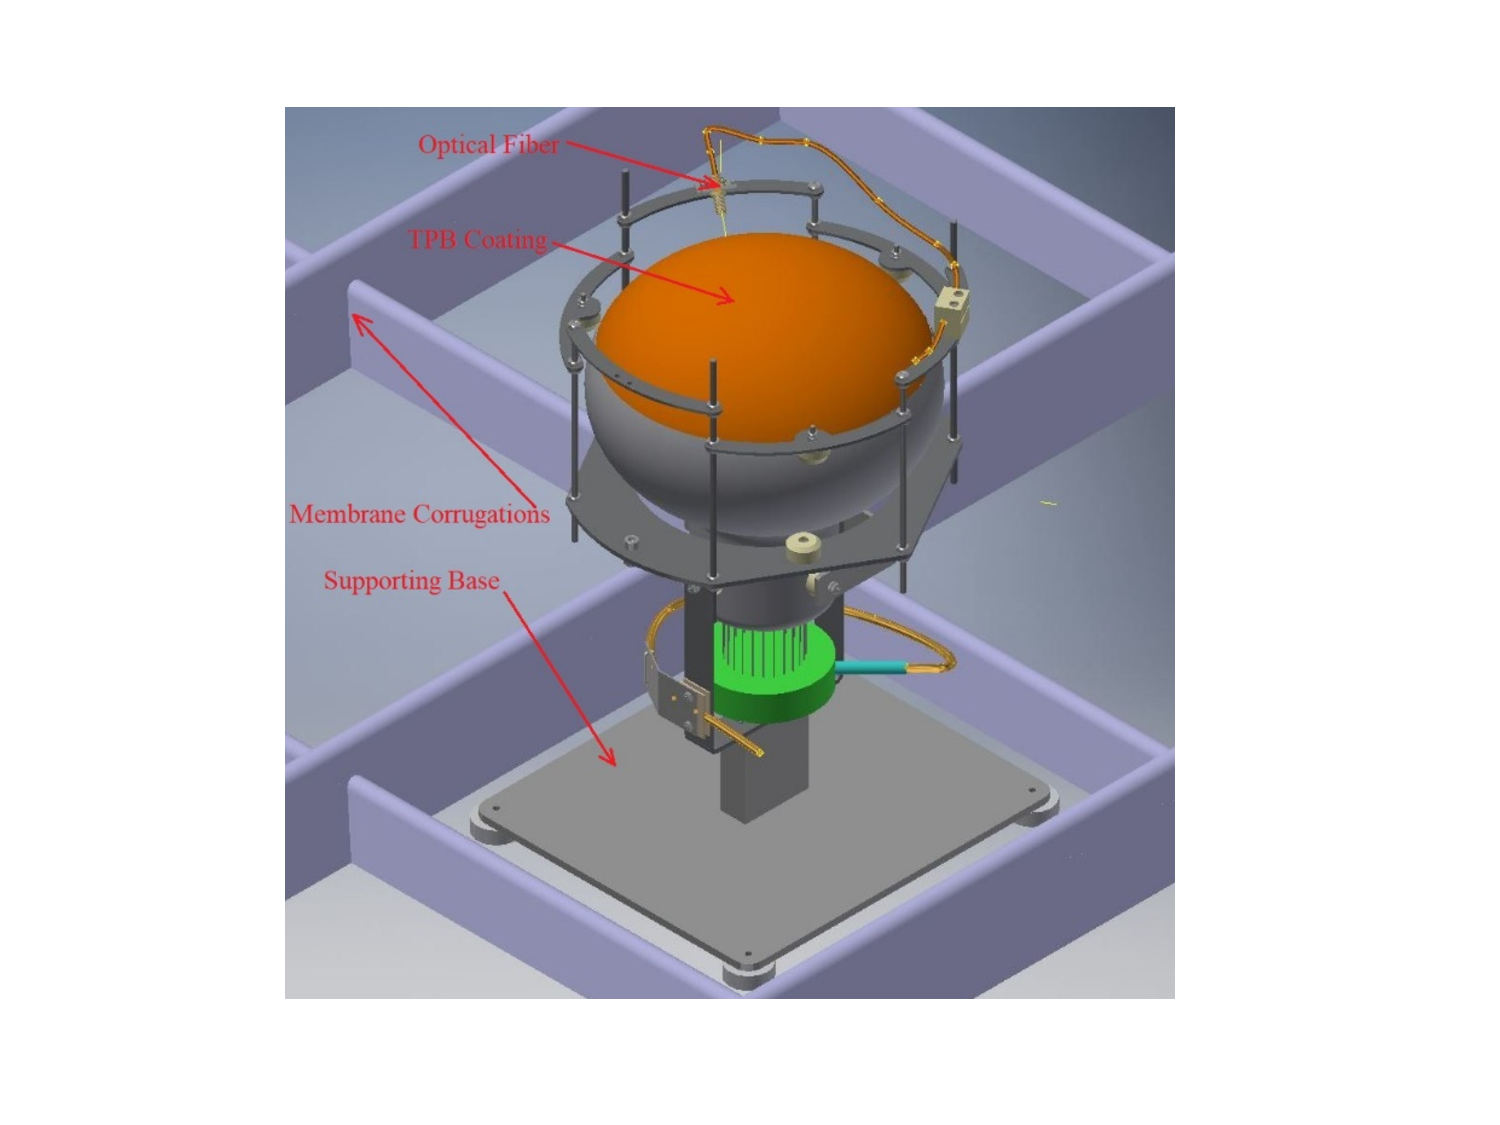
\includegraphics[width=0.42\textwidth]{dppd_3_2}
\end{dunefigure}

%%%%%%%%%%%%%%%%%%%%%%%%%%%%%%%%%%%%%%%%%%%%%%%%%%%%%%%%%%%%%%%%%%%%
\section{Readout Electronics}
\label{sec:fddp-pd-4}

%%%%%%%%%%%%%%%%%%%%%%%%%%%%%%%%%
\subsection{Photomultiplier High Voltage Dividers}
\label{sec:fddp-pd-4.1}

%For the \dword{pmt} power supply, the cathode grounding and positive \dword{hv} applied to the anode was chosen for \dword{pddp}. A single cable is required for each \dword{pmt} to carry power and signal. This configuration requires half of the cables and \fdth{}s on the detector than the negative voltage configuration, which is a clear advantage since the number of \dwords{pmt} in the detector is large. In addition, the cathode grounding shows less dark counts than the anode grounding scheme. The drawback is that a coupling capacitor must be used to separate the \dword{hv} from the \dword{pmt} signal, but, this signal and power splitting can be done externally from the detector. Figure~\ref{fig:dppd_4_1} shows the positive power supply and cathode grounding scheme.
The \dword{pddp} \dword{pmt} power supply has a grounded cathode and positive \dword{hv} applied to the anode. A single cable for each \dword{pmt} carries both power and signal. This configuration, which requires half as many cables and \fdth{}s on the detector as would the negative voltage configuration, offers a clear advantage given the large number of \dwords{pmt} in the \dword{detmodule}. In addition, the cathode grounding shows fewer dark counts than the anode grounding scheme. Although a coupling capacitor must be used to separate the \dword{hv} from the \dword{pmt} signal, this signal and power splitting can be done externally, mitigating this drawback.  Figure~\ref{fig:dppd_4_1} shows the positive power supply and cathode grounding scheme.

\begin{dunefigure}[Positive power supply and cathode grounding scheme.]{fig:dppd_4_1}
{Positive power supply and cathode grounding scheme.}
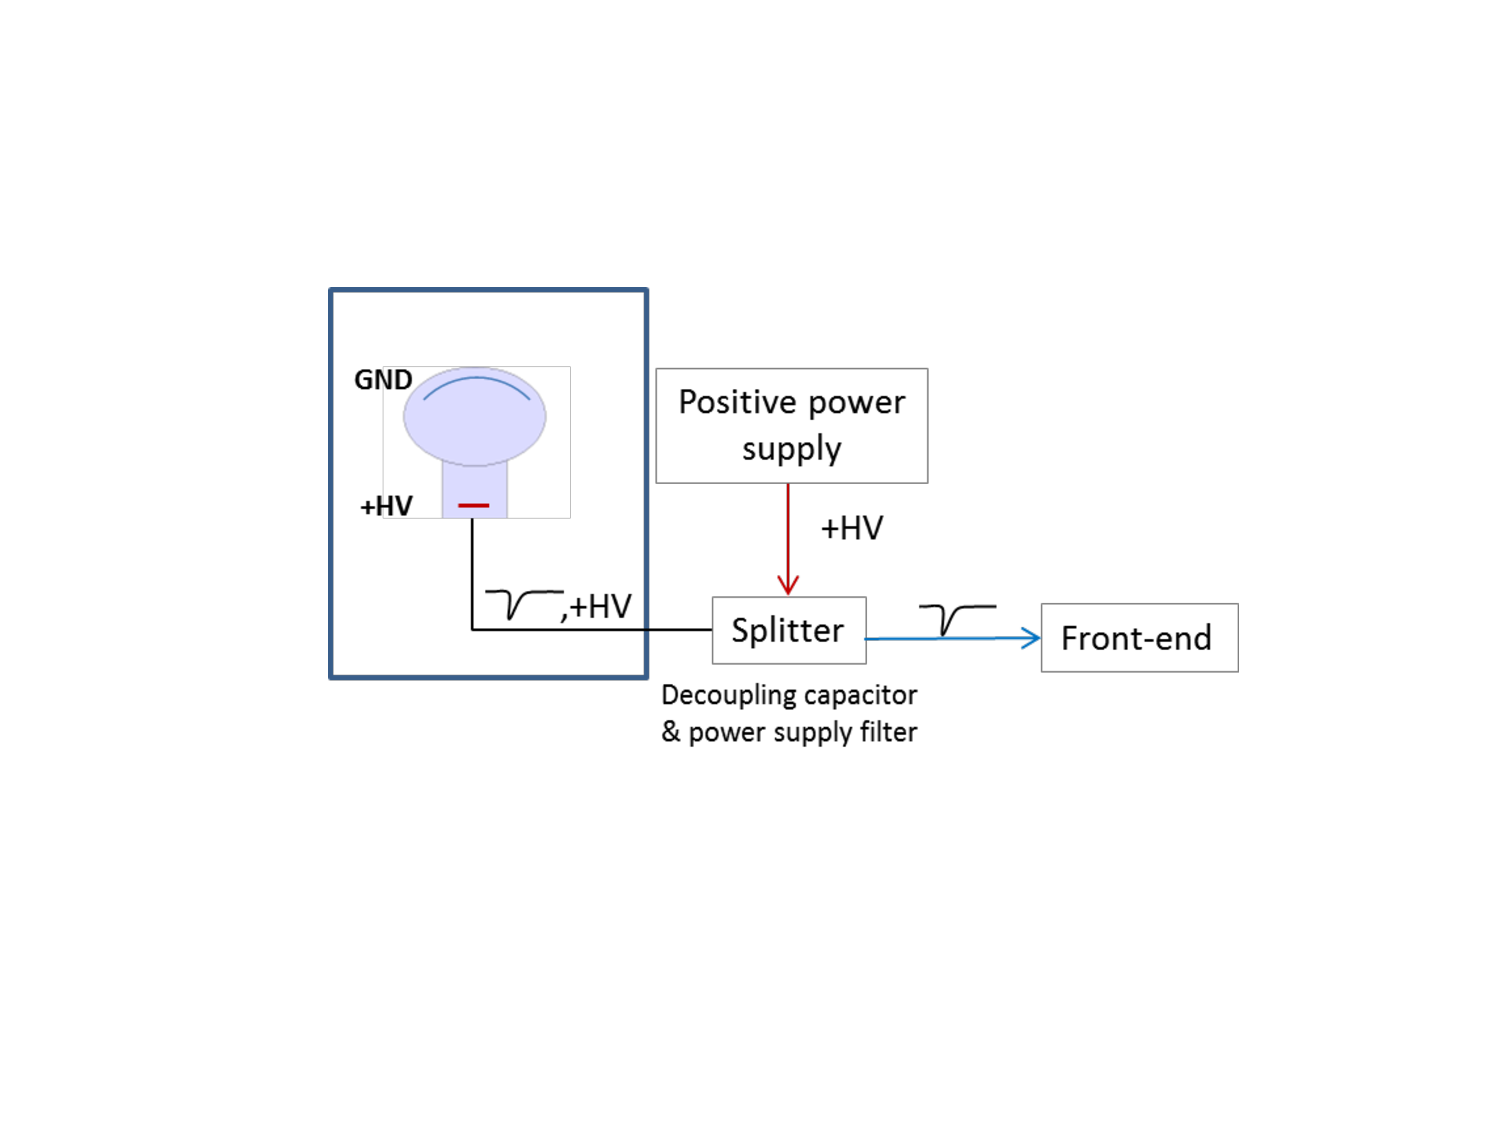
\includegraphics[width=0.5\textwidth]{dppd_4_1}
\end{dunefigure}

%The \dword{pmt} base circuit will be based only on resistors and capacitors as semiconductors do not work well in cryogenic temperatures. Nevertheless, the components will be carefully selected and tested to minimize the variations in their characteristics with temperature. The polarization current of the voltage divider (total circuit resistance) will be chosen to meet the \dword{pmt} light linearity range and maximum power requirements. The dynodes voltage ratio will follow the manufacturer recommendations for increased linearity range on the space-charge effect area (tapered divider). In addition, capacitors will be added to the last stages to increase the \dword{pmt} linearity in pulsed mode. The precise values for the components have not been decided yet as they depend on concrete requirements and also on the results from \dword{pddp}. The \dword{pddp} base design is considered as the baseline solution.
The \dword{pmt} base circuit uses only resistors and capacitors, as semiconductors do not work well in cryogenic temperatures. The components are carefully selected and tested to minimize the variations in their characteristics with temperature. The polarization current of the voltage divider (total circuit resistance) is chosen to meet the \dword{pmt} light linearity range and maximum power requirements. The dynodes' voltage ratio will follow the manufacturer recommendations for increased linearity range on the space-charge effect area (tapered divider). In addition, capacitors are added to the last stages to increase the \dword{pmt} linearity in pulsed mode. The precise values for the components have not been decided yet, as they depend on concrete requirements and also on the results from \dword{pddp}. The \dword{pddp} %base 
design is considered as the baseline solution.

For the connection between the \dword{pmt} base and the \fdth, the RG-303/U cable was selected for its low attenuation and its proven reliability in cryogenic environments. %On one side, t
This cable is directly soldered to the \dword{pmt} base on one side, and it ends with an SHV connector on the other side for attachment to the flange. 

%%%%%%%%%%%%%%%%%%%%%%%%%%%%%%%%%
\subsection{High Voltage and Signal Splitters}
\label{sec:fddp-pd-4.2}

HV/signal splitters %will 
\fixme{I don't understand why slash is used (anne)}
are used to separate the fast \dword{pmt} response signal from the positive \dword{hv} with capacitive decoupling. %In addition, they will include 
A low-pass filter between the \dword{hv} supply and the \dword{pmt} %to 
reduces the noise.

%Radiated electromagnetic interference (EMI) picked-up by the cables and conducted noise from the \dword{hv} power supply can be synchronous across many \dword{pmt} channels (coherent noise) that could be added-up producing false detector triggers. As the \dword{pmt} signal can be as low as few mV, another important issue is the control of the EMI over the circuit. The EMI induced and conducted by the power supply cables will be reduced by the splitter \dword{hv} input filter. To reduce the EMI directly received in the splitter circuit as well as the cross-talk between different splitter channels, each splitter channel will be enclosed into an individual metallic grounded box.
It is possible for radiated electromagnetic interference (EMI) picked up by the cables and conducted noise from the \dword{hv} power supply to be synchronous across many \dword{pmt} channels (i.e., coherent noise). This noise could add up to produce false detector triggers. Since the \dword{pmt} signal can be as low as few \si{mV}, %another important issue is the 
control of the EMI over the circuit is very important. The splitter \dword{hv} input filter is intended to reduce the EMI induced and conducted by the power supply cables. Enclosing each splitter channel in its own metallic grounded box will reduce the EMI directly received in the splitter circuit and %as well as 
the cross-talk between different splitter channels.

Figure \ref{fig:dppd_4_2} shows a generic splitter circuit where R1 and C1 form the \dword{hv} input low-pass filter (with a cut-off frequency below \SI{60}{Hz}). The resistor R7 and the  \dword{led} are for safety purposes only, warning when \dword{hv} is applied to the splitter. The C4 capacitor splits the signal coming from the \dword{pmt} from the \dword{hv}, and R2 prevents the \dword{pmt} signal from going to ground through the C1 capacitor. R4 and R5 are zero \si{\ohm} optional resistors that allow some flexibility in the grounding configuration. Finally, R3 ensures the discharging of C4 if the splitter is not connected to the \SI{50}{\ohm} input at the \dword{daq} system. The RC constant of the capacitor C4 and the load (\SI{50}{\ohm}) must be as large as possible to minimize baseline oscillations due to the charge-discharge of the capacitor. Values of C4 between \SI{150}{nF} and \SI{300}{nF} have already been tested in  \dword{wa105}. % $3\times1\times1$\,m$^3$ detector.

\begin{dunefigure}[Generic splitter circuit diagram.]{fig:dppd_4_2}
{Generic splitter circuit diagram.}
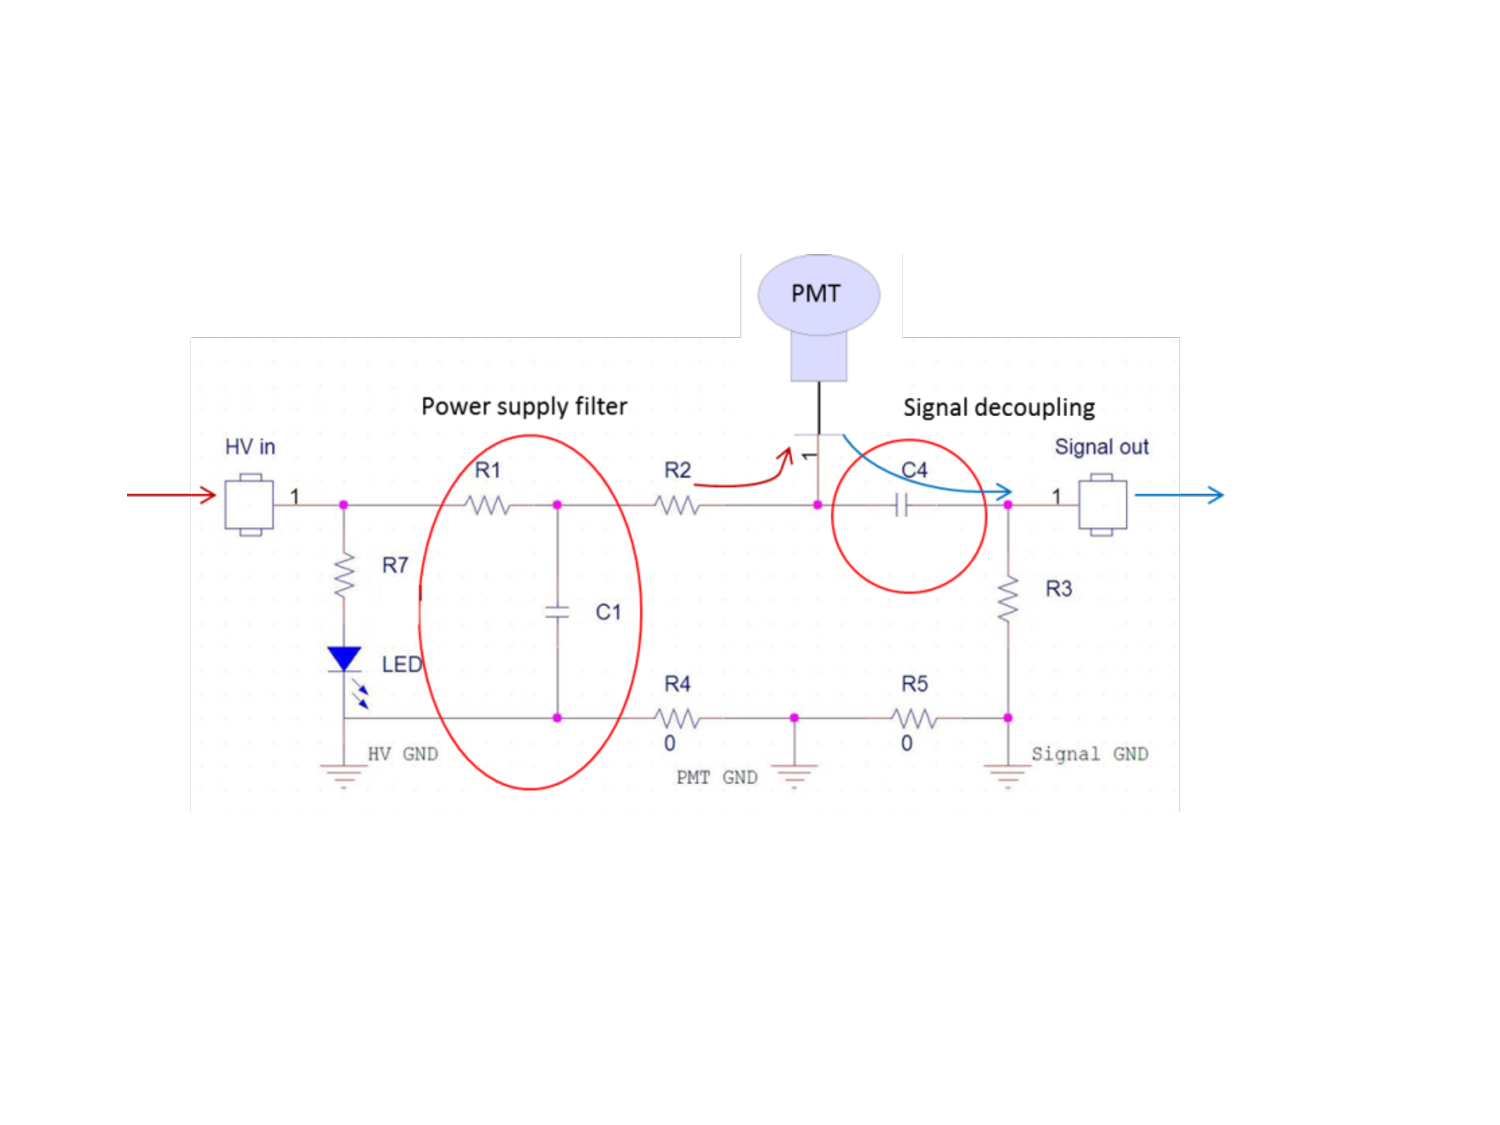
\includegraphics[width=0.75\textwidth]{dppd_4_2}
\end{dunefigure}

For the connections between the \dword{hv} power supply and the splitters and, also, between the splitters and the cryostat \fdth{}s, the HTC 50-3-2 cable have been chosen as baseline. The HTC 50-3-2 has a similar attenuation %compared to 
as the RG-303/U (used inside the cryostat), but with a factor of \numrange{8}{10} lower cost. Both cables will be attached on one side directly to the \dword{hv} splitter and will have an SHV connector on the other end. For the connection between the splitter and the \dword{fe}, an RG-58 cable %ended 
terminated on the connector required by the \dword{fe} card is used.

%%%%%%%%%%%%%%%%%%%%%%%%%%%%%%%%%
\subsection{Signal Readout Requirements}
\label{sec:fddp-pd-4.3}

In order to meet the physics requirements, the information that needs to be extracted from the \dword{pmt} signals is the following:

\begin{itemize}
\item S1 fast component shape, charge and timing;
\item S1 slow component shape;
\item S2 shape, charge and timing (distance from S1 and duration);
\item Single \phel (SPE) charge spectrum for gain calculation during \dword{pmt} calibration;
\item Trigger signal generation by the coincidence of several \dword{pmt} signals.
\end{itemize}

%At this moment, we do not have an estimate of the \textbf{dynamic range }of the light that could reach the \dwords{pmt} on the \dword{dpmod}. Our calculations are based on the signals detected by the \dwords{pmt} on the  \dword{wa105} $3\times1\times1$\,m$^3$ detector. Although this prototype has a different dimension from the \dword{dpmod}, it is the only reference that we have for these estimates, until the \dword{pddp} detector and simulations are operational.
There is currently no estimate on the \textit{dynamic range} of the light expected to reach the \dwords{pmt} in the \dword{dpmod}. Our calculations are based on the signals detected by the \dwords{pmt} in \dword{wa105}, % $3\times1\times1$\,m$^3$ detector. Although this prototype has a 
which has quite different dimensions from the \dword{dpmod}. However it is the only available reference %that we have for these estimates, 
until the \dword{pddp} and simulations are operational.

%In general, the \dword{pmt} signal dynamic range goes from the mV level to several volts (over \SI{50}{$\Omega$} load). During the operation of the  \dword{wa105} $3\times1\times1$\,m$^3$ detector, \dword{pmt} signals larger than \SI{2}{V} were observed with \dword{pmt} gains around \num{10}$^6$. Figure~\ref{fig:dppd_4_3_ab} shows the SPE waveforms (left, normalized) and amplitudes (right) for the  \dword{wa105} $3\times1\times1$\,m$^3$ detector at different voltages. The light levels in the \dword{dpmod} will have a larger dynamic range due to its large volume, so, higher gains will be required to see the far light signals. However, higher gains will make closer light signals to produce larger outputs, so, it is also essential that the \dword{fe} electronics can cover a large range of input voltages. To cover a dynamic range of \SI{10}{V} with a resolution below the mV level, \num{14} bits will be necessary (least significant bit (LSV) $\sim$\SI{0.6}{mV}). For \SI{2}{V} of dynamic range \num{12} bits would be sufficient (LSB $\sim$\SI{0.5}{mV}). To finalize the required dynamic range, results from \dword{pddp} and relevant simulations are needed.
In general, the \dword{pmt} signal dynamic range goes from the \si{mV} level to several volts (over \SI{50}{\ohm} load). During the operation of \dword{wa105}, \dword{pmt} signals larger than \SI{2}{V} were observed with \dword{pmt} gains around \num{e6}. %\num{10}$^6$. 
Figure~\ref{fig:dppd_4_3_ab} shows the SPE waveforms (left, normalized) and amplitudes (right) for \dword{wa105} at different voltages. The light levels in the \dword{dpmod} will have a larger dynamic range due to its large volume, therefore higher gains are required to see the far light signals. However, higher gains increase the output from closer light signals, requiring that the \dword{fe} electronics cover a large range of input voltages. To cover a dynamic range of \SI{10}{V} with a resolution below the \si{mV} level, \num{14} bits are necessary (least significant bit (LSV) $\sim$\SI{0.6}{mV}). For \SI{2}{V} of dynamic range \num{12} bits would be sufficient (LSB $\sim$\SI{0.5}{mV}). Results from \dword{pddp} and relevant simulations are needed to determine the required dynamic range.

\begin{dunefigure}[SPE waveforms and amplitudes from \dword{wa105} at different voltages.]{fig:dppd_4_3_ab}
{SPE waveforms (left) (normalized for comparison) and amplitudes (right) from the \dword{wa105} detector at different voltages.}
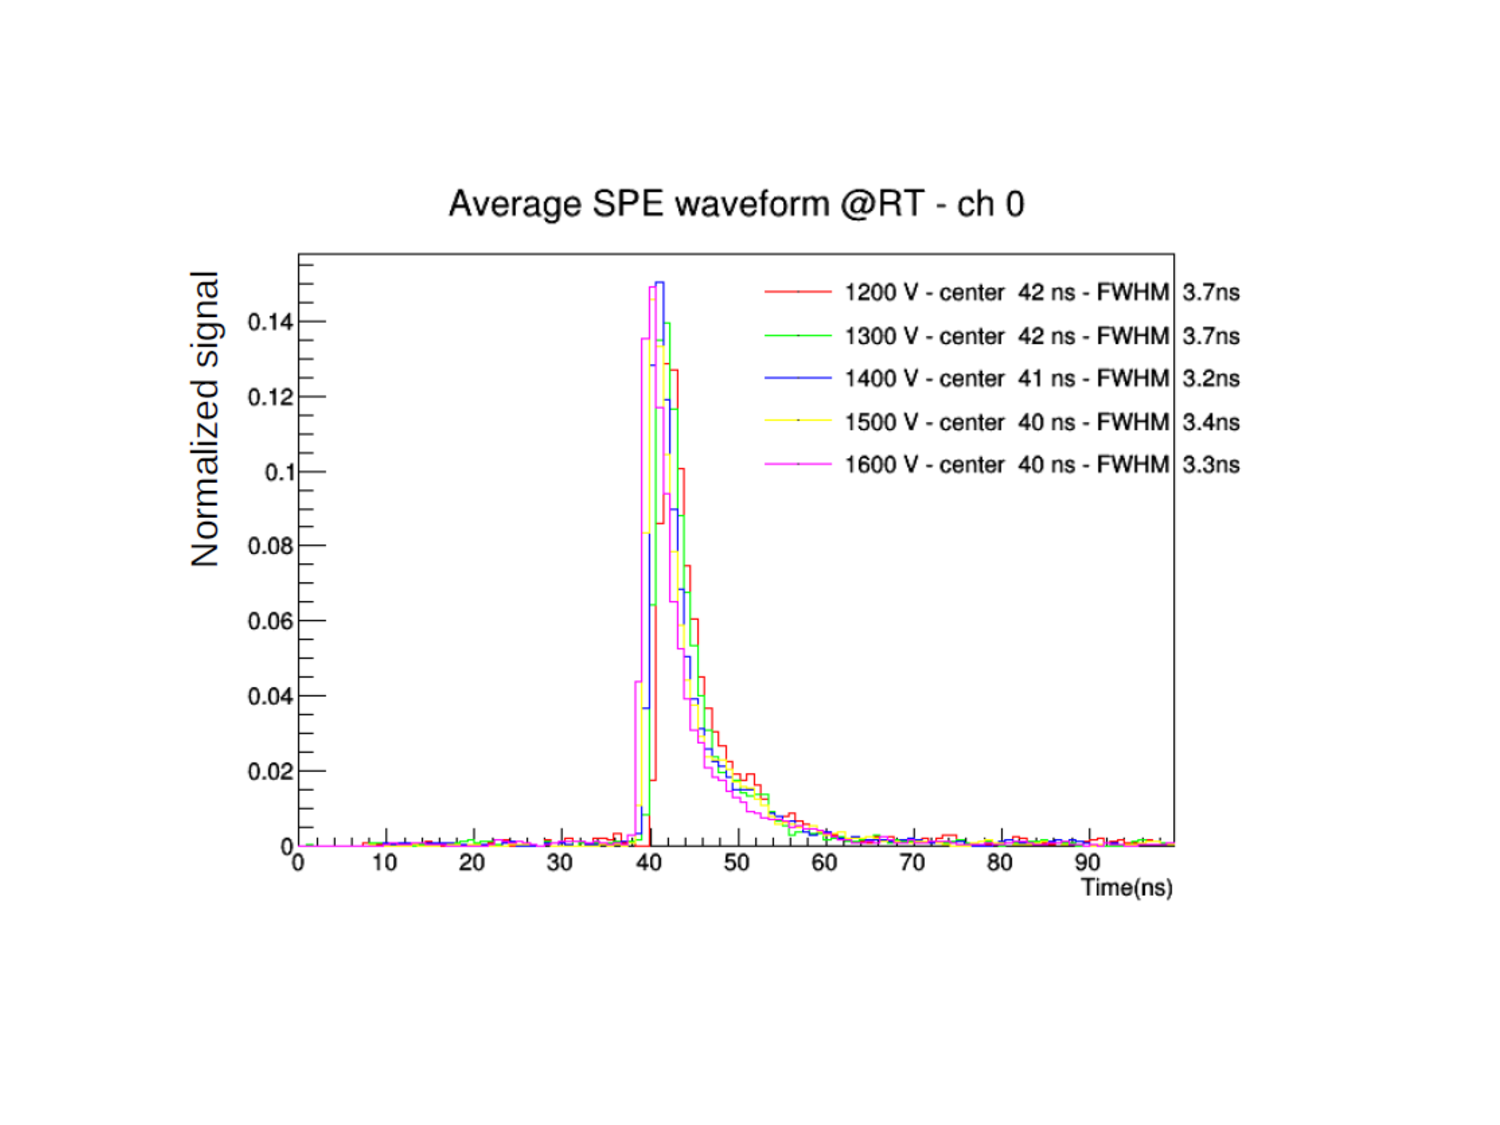
\includegraphics[width=0.47\textwidth]{dppd_4_3_a}
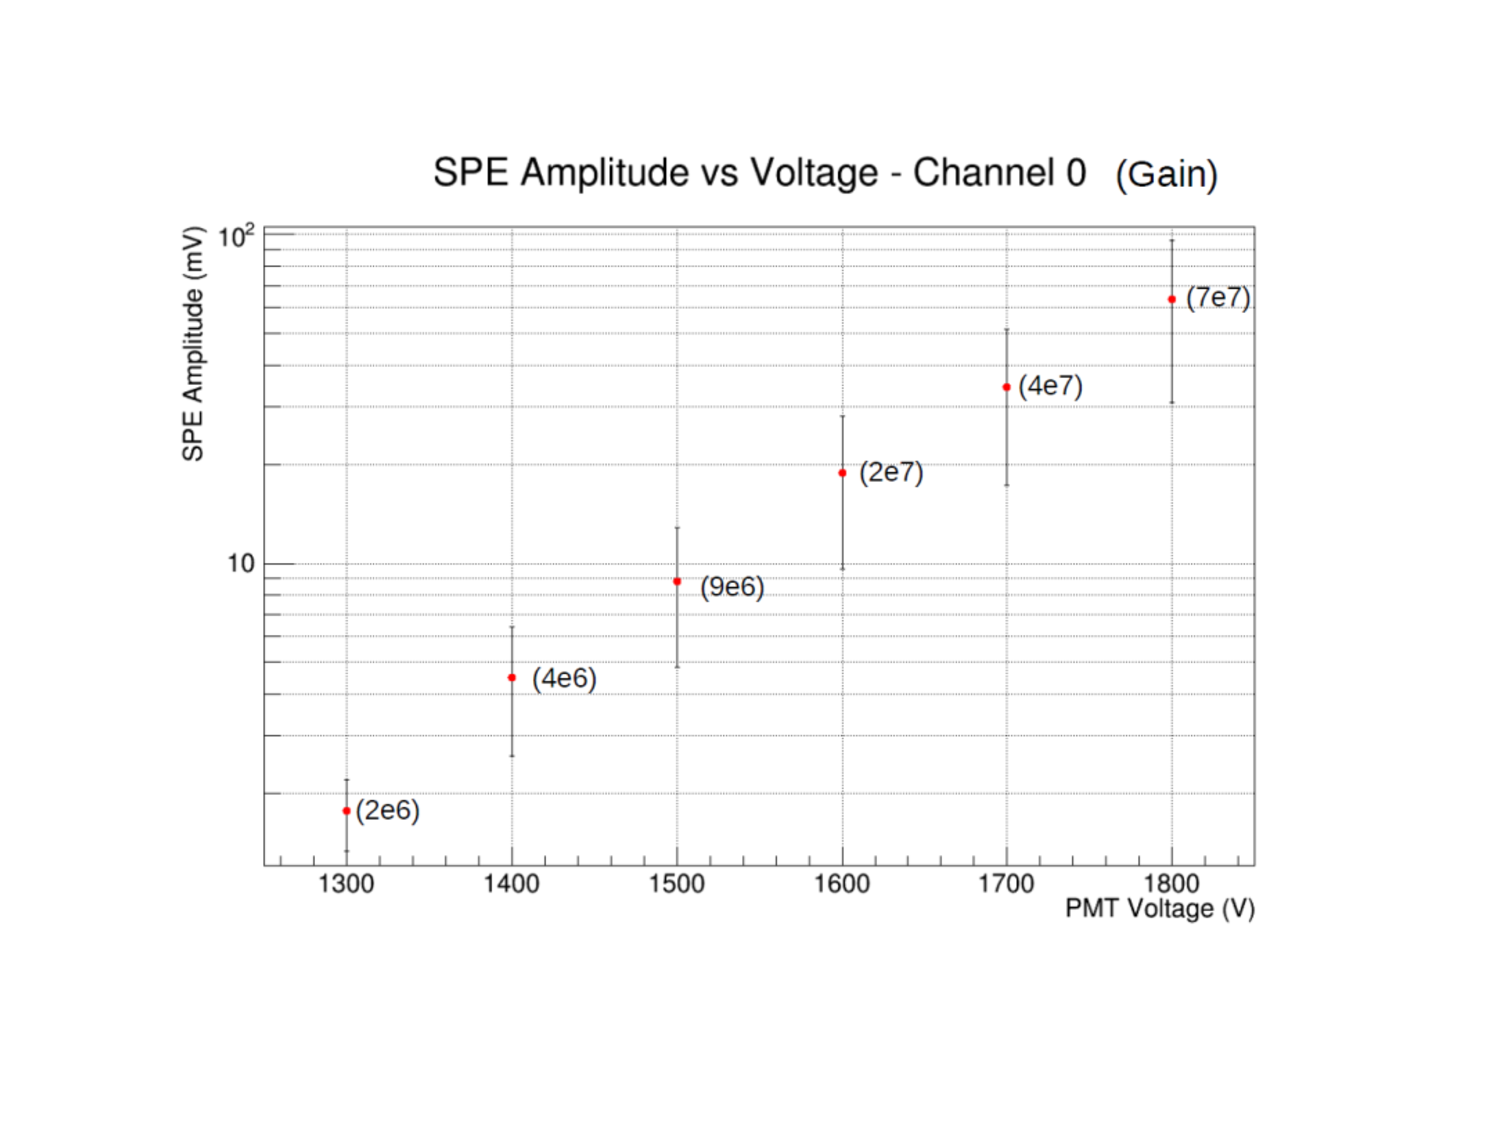
\includegraphics[width=0.47\textwidth]{dppd_4_3_b}
\end{dunefigure}

To calculate the \dword{pmt} gains, the SPE charge measurement will be performed. Depending on the \dword{pmt} gain, the SPE amplitude varies from the \si{mV} level to hundreds of \si{mV}, as shown in Figure~\ref{fig:dppd_4_3_ab}. Due to the very long cables from the \dwords{pmt} to the \dword{fe} electronics, the noise into the cables could be high. If one considers a noise level around \SI{1}{mV},  the \dword{pmt} gain must be set to \num{e6} or higher in order to distinguish the SPE from noise. The average SPE pulse width is around \SI{3.5}{ns} full width at half maximum (FWHM). In order to digitize this signal to reconstruct it with fidelity, a sampling period on the order of \SI{}{ns} is required.

The \textit{sampling frequency} also affects the time tagging precision. The time uncertainty due to the \dword{pmt} alone is around \SI{3}{ns} (transit time spread). Other factors, e.g., Rayleigh scattering, will increase this uncertainty, as will the sampling period; therefore, the lower sampling frequency, the better. In the  \dword{wa105} \SI{4}{ns} sampling was used to digitize waveforms. 

The rate of the events observed in \dword{wa105} was around \SI{300}{kHz} with the threshold at the SPE level. The rate at the \dword{dpmod}, is not yet known, but expected to be much larger despite the underground location. The time-tagging system needs to process events at high rates to ensure that no events are lost. Figure~\ref{fig:dppd_4_3_c} shows the event rates for different trigger thresholds observed in \dword{wa105}.

\begin{dunefigure}[Event rates for different trigger thresholds observed in  \dword{wa105}.]{fig:dppd_4_3_c}
{Event rates for different trigger thresholds observed in \dword{wa105} .}
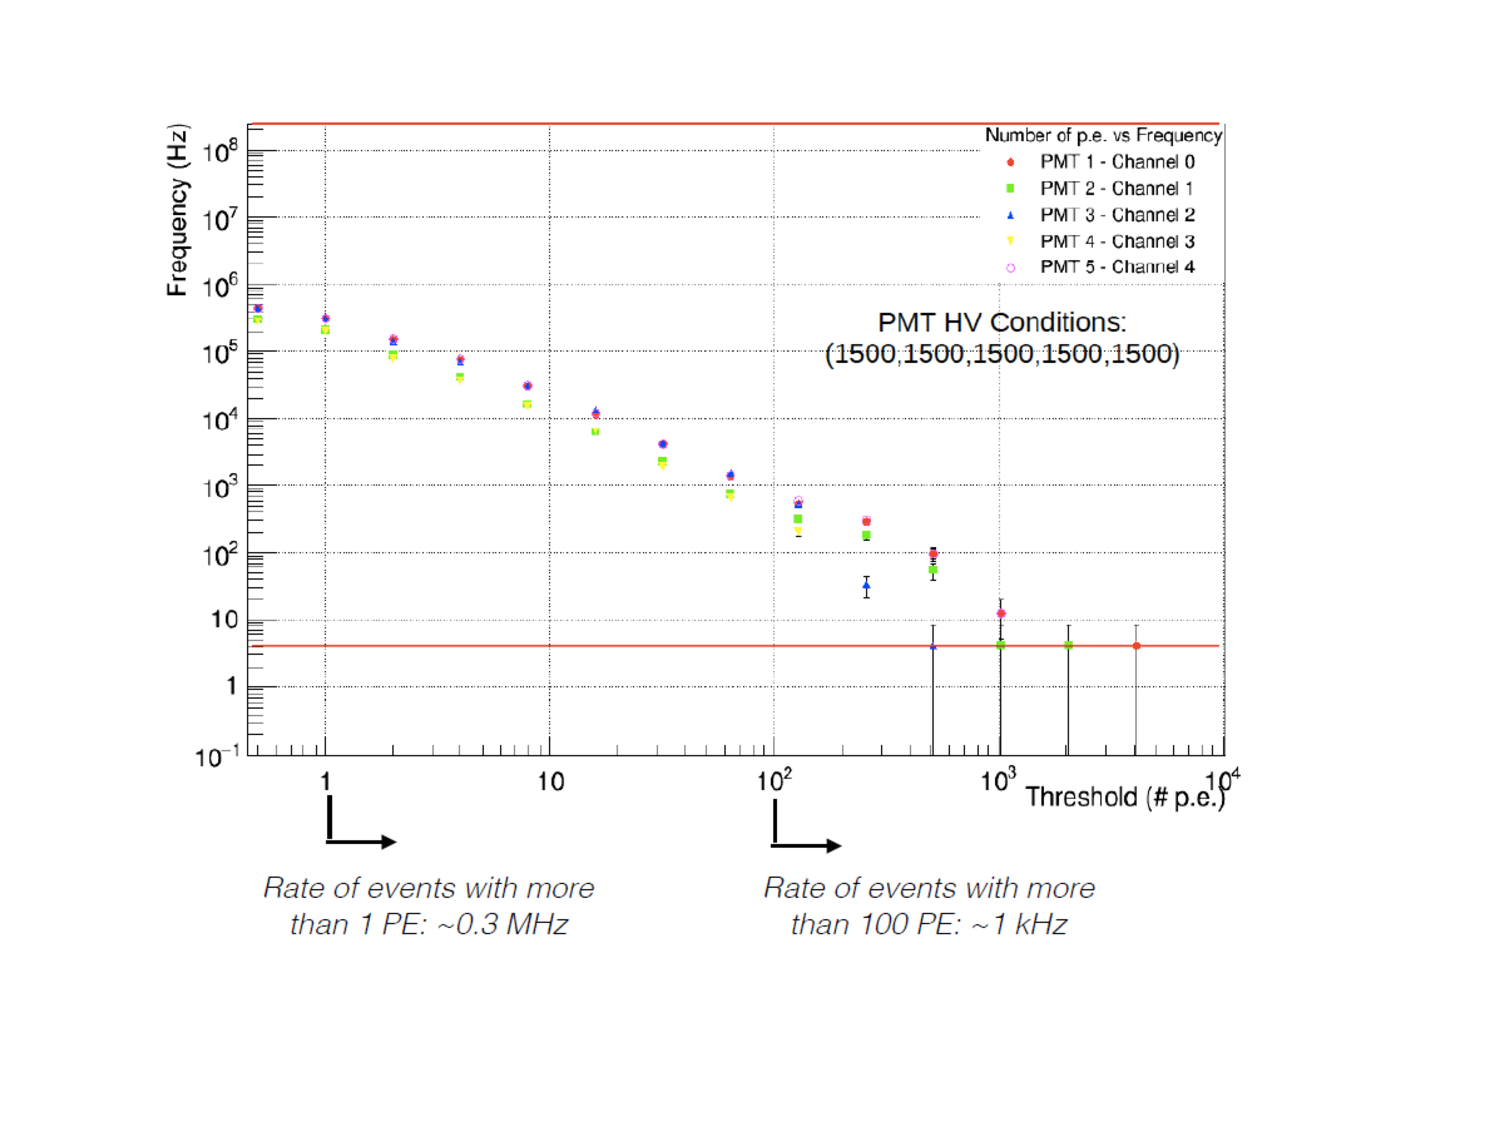
\includegraphics[width=0.6\textwidth]{dppd_4_3_c}
\end{dunefigure}

The light signal has to be \textbf{synchronized} with the \dword{daq}. All the \dword{daq} electronics use the \dword{wr} protocol for synching. %will be in sync using White Rabbit protocol. 
A dedicated \dword{wr} \dword{utca}~\cite{utca} slave node will be on the light readout \dword{fe} electronics as sync receiver, distributing clocks to the different \dword{fe} cards.

%%%%%%%%%%%%%%%%%%%%%%%%%%%%%%%%%%%%%%%%%%%%%%%%%%%%%%%%%%%%%%%%%%%%
\section{Photon Calibration System}
\label{sec:fddp-pd-5}

%%%%%%%%%%%%%%%%%%%%%%%%%%%%%%%%%
\subsection{System Design and Procurement}
\label{sec:fddp-pd-5.1}

A photon calibration system is required to be integrated into the \dword{dpmod}  to monitor the calibration of the \dwords{pmt} 
\fixme{to monitor the calibration of?}
installed in the \lar volume. The goal is to determine the \dword{pmt} gain and maintain the \dword{pmt} performance stability. A design similar to the one used in \dword{pddp} will be used although some R\&D measurements are planned to make it more effective, reduce the cost and mitigate issues related to the scaling.

%In \dword{pddp}, an optical fiber will be installed at each \dword{pmt} in order to provide a configurable amount of light (see Figure~\ref{fig:dppd_3_2}). The calibration light will be provided by a blue  \dword{led} of \SI{460}{nm} using a Kapuschinski circuit as  \dword{led} driver which reduces significantly the cost of using a laser. There will be one  \dword{led} connected to one fiber going to one female optical \fdth from Allectra~\cite{allectra}. In total,  there will be six  \dwords{led} placed in a hexagonal geometry. The direct light will go to the fiber, and the stray light to a SiPM used as reference sensor, being a single reference sensor in the center. Fibers of length 22.5-m (from Thorlabs $\phi$ 800-$\mu$m, FT800UMT~\cite{ft800umt}, and stainless-steel jacket) will be used inside the cryostat. Each one of these fibers will be attached to a 1-to-7 fiber bundle (from Thorlabs $\phi$ 200-$\mu$m, FT200UMT~\cite{ft200umt}, stainless-steel jacket common end, and black jacket at split ends), so that one fiber is finally installed at each \dword{pmt}. A diagram of the \dword{pddp} photon calibration system is shown in Figure~\ref{fig:dppd_5_1}. Several tests to quantify the light losses of this design were performed with successful results. 
In \dword{pddp}, an optical fiber is installed at each \dword{pmt} in order to provide a configurable amount of light (see Figure~\ref{fig:dppd_3_2}). The calibration light is provided by a blue  \dword{led} of \SI{460}{nm} using a Kapuschinski circuit as  \dword{led} driver; this reduces significantly the cost of using a laser.
\fixme{is much less expensive than using a laser?}
One \dword{led} is connected to one fiber that goes to one female optical \fdth from Allectra~\footnote{Allectra\texttrademark{}, \url{http://www.allectra.com/index.php/en/}.} %\cite{allectra}. 
In total,  six  \dwords{led} are placed in a hexagonal geometry. The direct light goes to the fiber, and the stray light to a \dword{sipm} used as a single reference sensor %, being a single reference sensor 
in the center. Fibers of length \SI{22.5}{m} (from Thorlabs $\phi$ \SI{800}{\micro\meter}, FT800UMT,~\footnote{Thorlabs\texttrademark{}, \url{https://www.thorlabs.com/thorproduct.cfm?partnumber=FT800UMT}.} %~\cite{ft800umt},
 and stainless-steel jacket) are used inside the cryostat. Each of these fibers is attached to a \numrange{1}{7}-fiber bundle (from Thorlabs $\phi$ \SI{200}{\micro\meter}, FT200UMT~~\footnote{Thorlabs\texttrademark{}, \url{https://www.thorlabs.com/thorproduct.cfm?partnumber=FT200UMT}.} %\cite{ft200umt}, 
 stainless-steel jacket common end, and black jacket at split ends), so that one fiber is finally installed at each \dword{pmt}. A diagram of the \dword{pddp} photon calibration system is shown in Figure~\ref{fig:dppd_5_1}. Several tests to quantify the light losses of this design were performed with successful results. \fixme{citation?}

%%% anne to here 5/2 4pm
\begin{dunefigure}[Diagram of the photon calibration system to be implemented in \dword{pddp}.]{fig:dppd_5_1}
{Diagram of the photon calibration system to be implemented in \dword{pddp}}
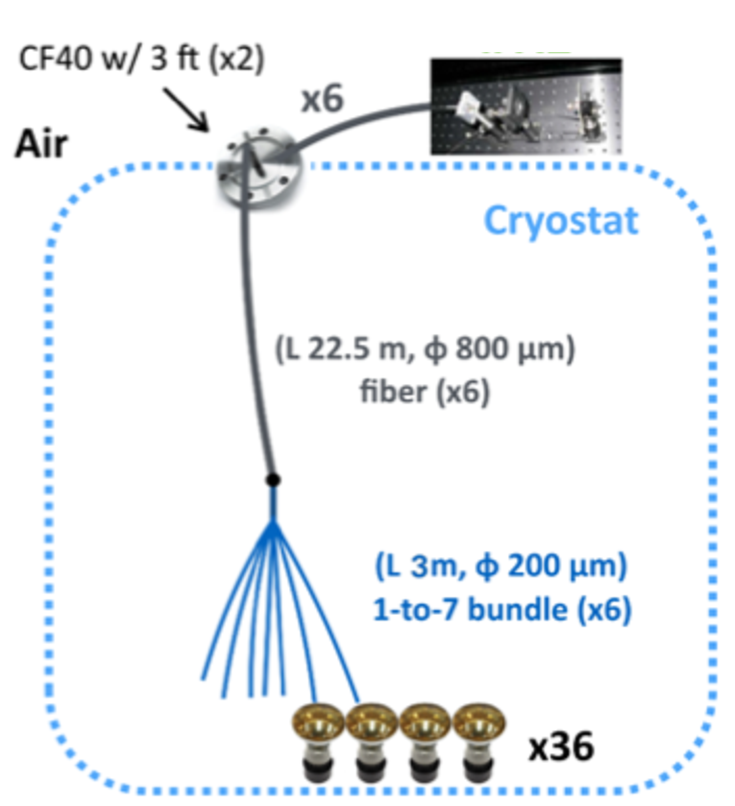
\includegraphics[width=0.4\textwidth]{dppd_5_1}
\end{dunefigure}

Assuming the \dword{pddp} design for the DUNE FD with \num{720} \dwords{pmt}, \num{120} bundles, \num{120} fibers, \num{120} light sources, \num{120} flange \fdth{}s, and \num{20} reference sensors will be needed. The length of the fibers and bundles has to be calculated considering the exact position of the \fdth flanges. The number of flanges required to host \num{120} SMA \fdth{}s will depend on their size. However, alternatives to this design will be pursued with R\&D measurements in order to reduce the amount of fibers, study other options for the reference sensor, and increase the input light if necessary. In order to reduce the number of fibers, light diffusers can be used, so that one fiber can illuminate at least \num{4} \dwords{pmt}. For instance, a diffuser could be placed at the ground grid. 

%%%%%%%%%%%%%%%%%%%%%%%%%%%%%%%%%
\subsection{Validation Tests}
\label{sec:fddp-pd-5.2}

In order to validate the design, the most important result will come from the \dword{pddp} performance. In any case, since the fibers to be used in DUNE FD will be longer, dedicated calculations and measurements to confirm that sufficient light reaches the \dwords{pmt} will be performed. Also, alternative designs, will be validated in different laboratories. The possibility of using a diffuser can be tested in a vessel. The light source will also be validated by studying the different options in the lab. All these measurements will be performed at room temperature and in liquid nitrogen to test the behavior at cryogenic temperatures.

Once the design is fixed, basic characterization measurements will be performed on the fibers upon receiving them from the manufacturer. Those measurements will consist of providing light with a known source and measuring the output with a power meter. Measurements at cryogenic temperatures may not be needed at this point.

Finally, during the photon calibration system installation, each fiber and source will be re-tested to check that the expected light is arriving to each \dword{pmt} using a photodiode. A dedicated procedure will be designed with this purpose, similar to the one used in \dword{pddp}.

%%%%%%%%%%%%%%%%%%%%%%%%%%%%%%%%%%%%%%%%%%%%%%%%%%%%%%%%%%%%%%%%%%%%
\section{Photon Detector Performance}
\label{sec:fddp-pd-6}

To define the \dword{pds} performance, a good understanding of the light generation is needed. For this, optical simulations and a good knowledge of the light properties are required. The DUNE experiment expects to record not only accelerator neutrino interactions, but also rare non-beam events such as supernova neutrino bursts or nucleon decays. In those cases, an internal trigger is required: an optimized light collection system is hence mandatory. This section will describe the tools developed in the consortium for the light simulation in large detector volumes for these purposes.

The main feature of a \lartpc detector is to collect electrons produced by the energy loss of charged tracks when crossing the volume. This signal provides a high resolution 3D image of the event. The reconstructed topology and the amount of charge collected gives the characterization of the tracks (identification and energy). Together with the charge, scintillation light is also produced in \lar. There are many advantages to collect and exploit the scintillation signal. As only a fraction of the initial energy deposition is converted into electrons, the rest being emitted as photons, light collection can improve the calorimetry of the detector. The light signal can provide the $t_0$ of the event, which is a necessary observable for a proper reconstruction. The study of the slow component can give insights into the purity of the \lar. 

When energy deposition occurs, either the knocked argon atom gets excited or an electron is ejected. For the latter case, the electron has a probability to be recaptured by an argon ion, which depends on the drift field and on the amount of energy deposited. In this case, an excited argon state is also produced. In order to decay to ground state, the excited argon will combine with another argon atom, to form an excited eximer. A photon at \SI{127}{nm} will then be emitted to allow the eximer to return to ground state. As the eximer can be formed in a singlet or triplet state, two time constants will be observed: the singlet at \SI{6}{ns}
and the triplet at \SI{1.3}{$\mu$s}. These principles are sketched in Figure~\ref{fig:dppd_6_0}.

\begin{dunefigure}[A sketch depicting the mechanism of light production in argon.]{fig:dppd_6_0}
{A sketch depicting the mechanism of light production in argon.}
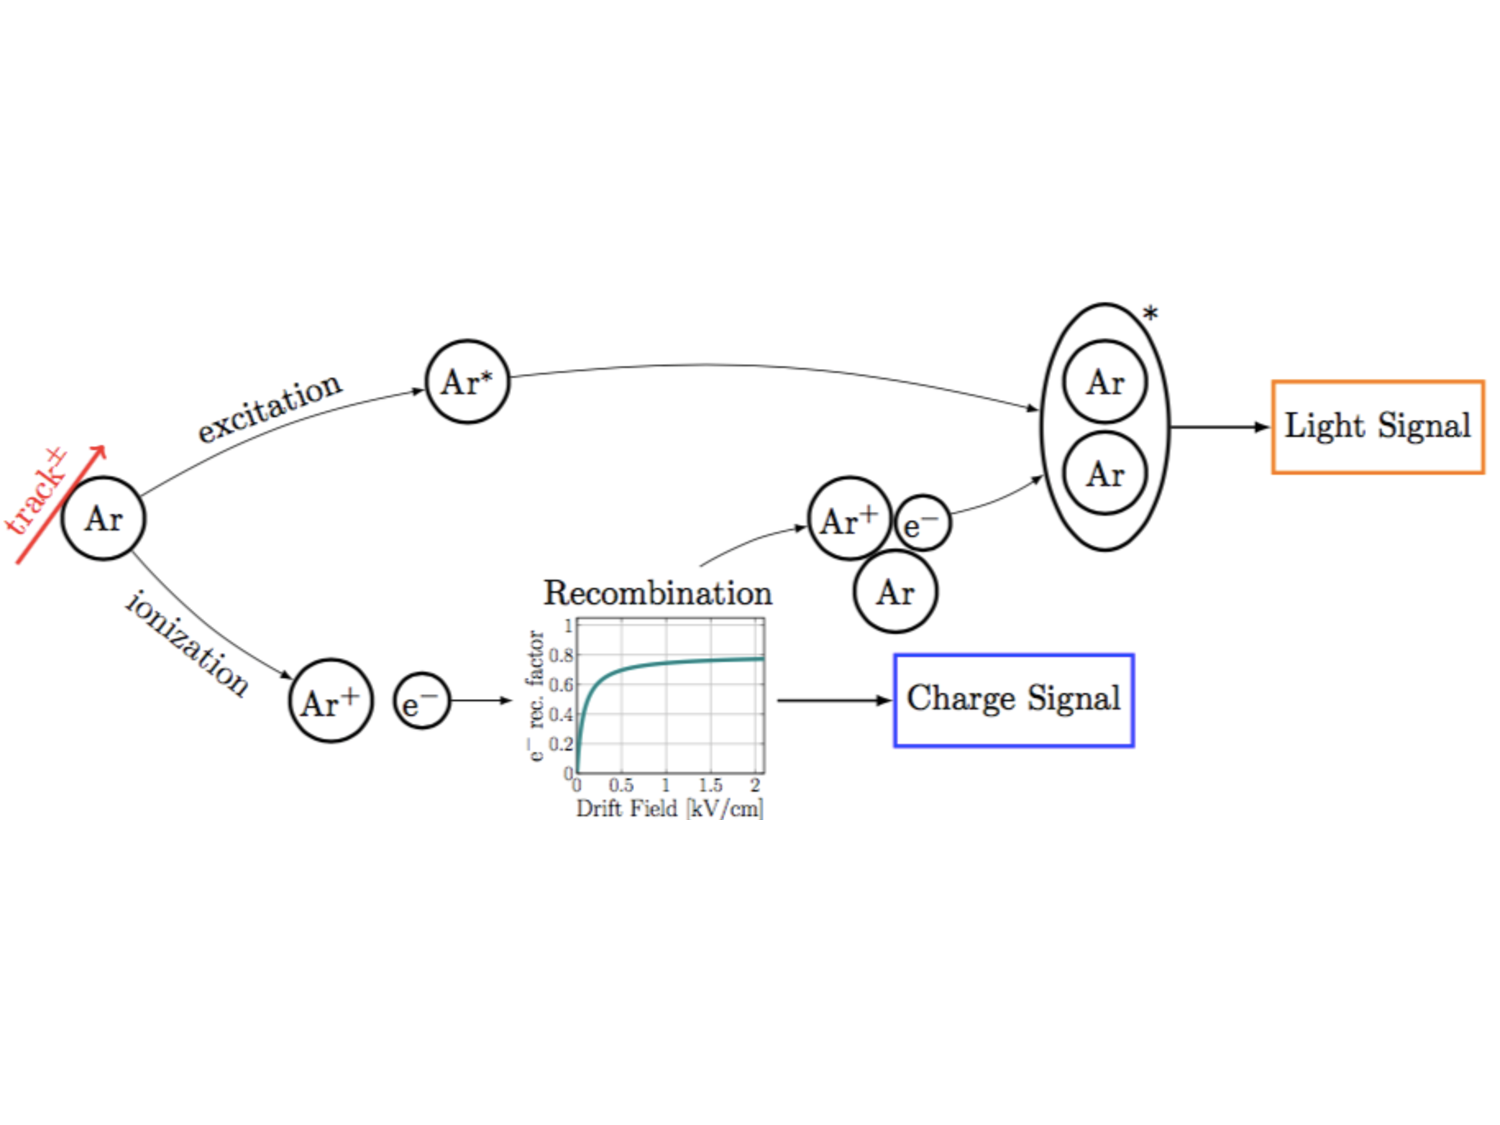
\includegraphics[width=0.8\textwidth]{dppd_6_0}
\end{dunefigure}

In the DP technology, due to the amplification area, there are two light signals produced. The first one, S1, is made by scintillation processes when a charged particle crosses the \lar volume. The second signal, S2, is produced in the gaseous phase. As the drifting electrons enter in high field regions (such as the extraction field or the amplification field in the \dwords{lem}), their velocities increase and Townsend avalanches occur. The current of electrons will produce electroluminescence light with the same wavelength and similar time structure as for the S1 signal. %The minimum field needed to produce electroluminescence is $\sim$\SI{3.5}{kV/cm} at the gas density at cryogenic temperatures. 
The S2 light is expected to be an irreducible background for the light studies in \dword{pddp}, as the detector will be on the surface. Indeed, the S2 signal can last as long as the total drift time of the electrons: \SI{0.625}{ms} per meter of drift at a drift field of \SI{500}{V/cm}.

Table~\ref{tab:dppd_t_6_0} summarizes the default optical parameters chosen for the light simulation methods described in the following subsection. The \lar optical properties are the subject of significant discussions in the community, in particular regarding the \lar absorption length and the Rayleigh scattering length. The former will affect the light yield collected whereas the latter will impact mostly its uniformity and timing resolution. The absorption/reflection of the VUV photons on stainless-steel (constituting the drift cage, cathode, extraction grid and ground grid) and on copper (on the \dword{lem} surfaces) are poorly known. The knowledge of those reflection coefficients is limited by the fact that they depend strongly on the polishing procedure. Hence, one cannot rely on the literature as the tooling will certainly be different. The measurement of the quantum efficiency of the \dwords{pmt} at vacuum ultra-violet (VUV) wavelengths requires a specific setup operating in vacuum as VUV photons are absorbed in air. For the construction of the   \dword{wa105} $3\times1\times1$\,m$^3$ detectorDP demonstrator, the \dword{pmt} quantum efficiencies were measured before and after the \dword{tpb} coating using an  \dword{led} that could emit light in the [\num{200}, \num{800}]\,nm range. Finally, the electroluminescence gain G, defined as the number of S2 photons produced per extracted drifting electron, is also subject to discussion. Experimental measurements of G have been performed in a setup quite similar to the amplification design of the DP technology, although the amount of photons emitted were measured above the \dword{lem}. In our case, the S2 photons are the ones leaving the \dword{lem} from below, which can be significantly lower. 

\begin{dunetable}
[Default optical properties. Below the thick line are presented some quantities used in our studies although they are not linked to the optical properties of the \lar.]
{lcc p{0.8\textwidth}}
{tab:dppd_t_6_0}
{Default optical properties. Below the thick line are presented some quantities used in our studies although they are not linked to the optical properties of the \lar.}
 & VUV photons & Shifted photons \\ 
 & $\lambda$ = \SI{127}{nm} & $\lambda$ = \SI{435}{nm}\\ \toprowrule
 Absorption length & \multicolumn{2}{c}{$\infty$} \\ \colhline
 Rayleigh scattering length & \SI{55}{cm} & \SI{350}{cm}\\ \colhline
 Absorption coefficients & \num{100}\% & \num{50}\% \\ \colhline
 \lar refractive index & \num{1.38} & \num{1.25}\\ \colhline
 \dword{pmt} quantum efficiency & \multicolumn{2}{c}{0.2 }\\ \colhline
 Electroluminescence gain & \num{300}\\ \colhline
\end{dunetable}

To understand the performance of the \dword{pds}, we need to take into account the following indicators:
\begin{itemize}
\item Overall detected light yield, in \phel{}s per MeV of deposited energy in \lar
\item Uniformity of the light yield across the entire \lartpc active volume
\item Event time resolution extracted from the detected photon signal 
\end{itemize}

In turn, these indicators will directly impact the strategy and performance of the DUNE trigger system (Sec.~\ref{sec:fddp-pd-7}), and will determine whether the \dword{pd} technical design is sufficient to meet the DUNE physics goals. These higher-level studies will be available on the TDR timescale. Our current understanding of the performance indicators listed above is largely based on \dword{pddp} simulations. The current status of the simulation work is discussed in detail in Sec.~\ref{sec:fddp-pd-6.1}, work is focused on \dword{pddp} in a first phase, and then will be expanded to DUNE DP FD. For a realistic \dword{pddp} geometry, an average light yield of \SI{2.5}{\phel{}s/MeV} is expected across the entire active volume. This promising yield is obtained  by assuming thirty-six 8-inch \dwords{pmt} located below the \dword{pddp} cathode plane, averaging to one \dword{pmt} per m$^2$. On the other hand, spatial non-uniformities in the \dword{pd} response are found to be important and need to be modeled in detail. Variations as large as one order of magnitude both parallel to the drift direction (due to geometrical effects and absorption of light by \lar) as well as perpendicular to it (due to light absorption on detector boundaries) are obtained. The event time resolution due to light production and light propagation times, hence neglecting electronics and \dword{daq} effects for now, is expected to be of order $\mathcal{O}$(\SI{100}{ns}) and hence largely sufficient for our purposes. These initial low-level performance estimates will be refined with more realistic simulations and with \dword{pddp} data (Sec.~\ref{sec:fddp-pd-6.2}) in the future. They will also be extended to the full FD geometry on the TDR timescale.

%%%%%%%%%%%%%%%%%%%%%%%%%%%%%%%%%
\subsection{Simulations}
\label{sec:fddp-pd-6.1}

At zero drift field, when the electron recombination is maximum, roughly \SI{40000}{$\gamma$/MeV} are produced. At the nominal drift field of \SI{500}{V/cm}, then \num{24000}{$\gamma$/MeV} are generated. For reference, the energy deposited by a minimum ionizing particle (MIP) track is \SI{2.12}{MeV/cm}. Given the size of the \dword{pddp} ($6\times6\times6$\,m$^3$) and the fact that it is located on surface, roughly \num{100} muons are expected to cross the fiducial volume during the \SI{4}{ms} time window of the data acquisition. With a full Geant4 \cite{geant4} simulation, it takes more than three hours to propagate all the photons emitted by a single MIP track crossing the \dword{pddp} detector. A full optical simulation is hence computationally prohibitive. Three simulation approaches are being explored to provide a light simulation needed for the design optimization of the DUNE FD module, described in the following.


\subsubsection{Generation of light maps}
\label{subsec:fddp-pd-6.1.1}

In this method, the photons are propagated in a full dedicated Geant4 simulation only once. The main light characteristics (photon detection probability called visibility hereafter, and time profile) needed for light studies are stored in a map in a ROOT \cite{root} file format which can then be read by any other simulation program. This work was done first using LightSim, a dedicated software developed at LAPP. These maps have been adapted to be read by \larsoft and work is on-going to directly generate them in \larsoft where light maps are known as photon libraries. In particular, S2 light needs to be simulated in \larsoft for the first time, as no previous effort on DP technology was done.

In the dedicated Geant4 code, special care has been taken to precisely describe all sub-detector components that might affect the light propagation: \dword{lem} plates, extraction grid, \dword{fc} rings, the cathode and its supporting structure and the ground grid above the \dwords{pmt}. The \lar fiducial volume is then divided into voxels of \SI{25}{cm^3} and \num{e8} photons are isotropically generated at the center of each voxel. The number of photons reaching each \dword{pmt}, and their arrival times are stored. The light map can then be built from these results. For each voxel and for each \dword{pmt}, the visibility is computed as: $w=N\gamma^{\textrm{collected}}/N\gamma^{\textrm{generated}}$. In order to be able to reproduce the time profile, each distribution is fit to a Landau function. From the fits, three parameters are extracted: the minimum time for photons to arrive to the \dword{pmt}, $t_0$; the peak of the distribution, $t_{\textrm{peak}}$ from the Landau most probable value (MPV); and the distribution spread, the $\sigma$ of the Landau function. These three parameters are stored in the light maps for each \dword{pd}. The same procedure is done for the gaseous phase, although the voxel size is smaller in height (only \SI{5}{mm}). In Figure~\ref{fig:dppd_6_1_1_ab}, two fitted time distributions are presented. As one can see, the shapes of the time distributions depend strongly on the source to \dword{pmt} distance. For close sources, the distributions are very sharp and the Landau description may not be the optimal function to use. On the other hand, when the distance is larger, the distribution is broader and the Landau fit reproduces the simulations quite well. In order to minimize the amount of parameters to be stored in the map, the Landau descriptions for all cases were kept as only a small fraction of the fits could be considered problematic.

\begin{dunefigure}[Landau fits (red line) of the travel time distributions (black histogram) for a source close (left) and far (right) to the \dword{pmt}.]{fig:dppd_6_1_1_ab}
{Landau fits (red line) of the travel time distributions (black histogram) for a source close (left) and far (right) to the \dword{pmt}.}
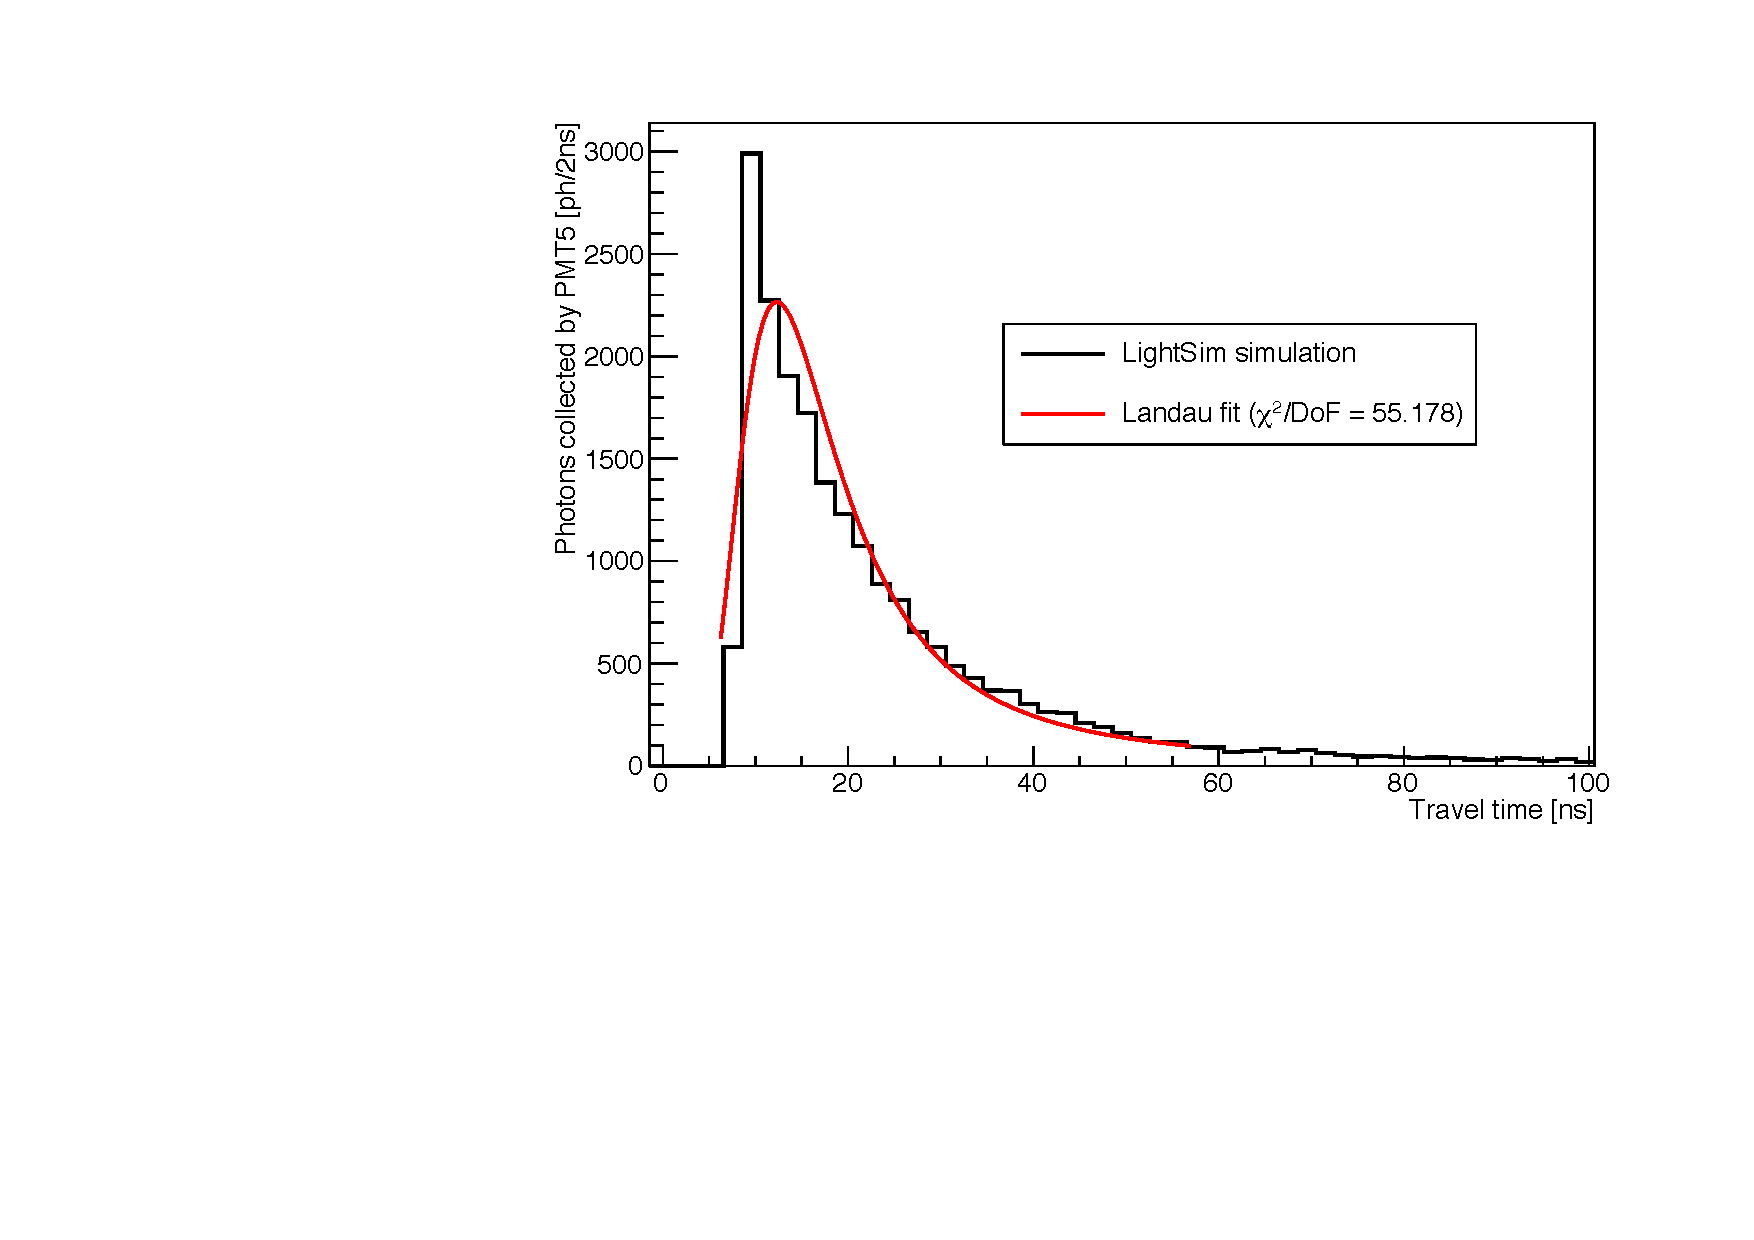
\includegraphics[width=0.45\textwidth]{dppd_6_1_1_a}
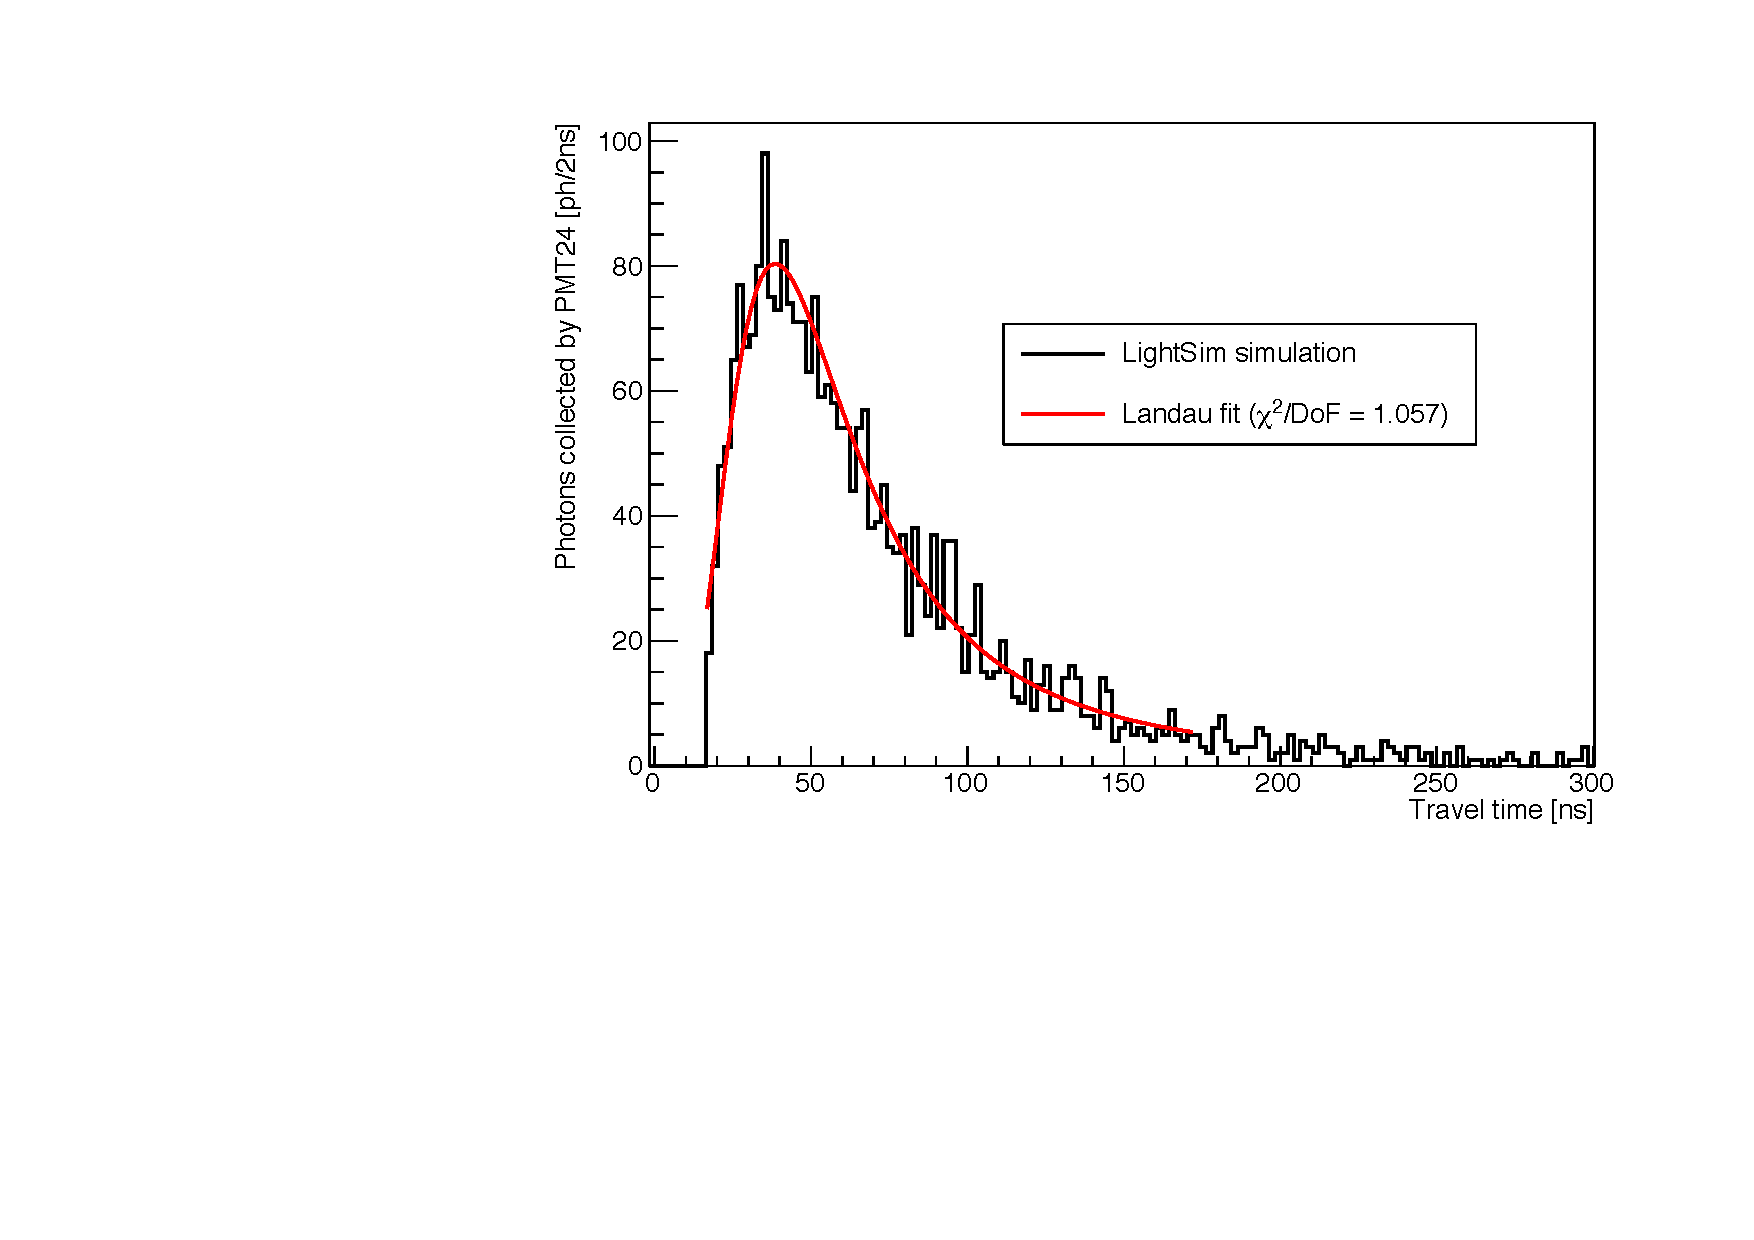
\includegraphics[width=0.45\textwidth]{dppd_6_1_1_b}
\end{dunefigure}

As the map has been computed with discrete entries, an interpolation of the four light parameters ($w$, $t_0$, $t_{\textrm{peak}}$, $\sigma$) between the actual source position and the closest voxel centers is performed. An example of the evolution of the visibility and its 3D interpolation is presented in Figure~\ref{fig:dppd_6_1_1_cd}. The loss of photons due to the cathode and ground grid are visible. Given the \dword{pddp} cathode and supporting structure design, and considering the default optical parameters presented in Table~\ref{tab:dppd_t_6_0}, it has been shown that up to $\sim$\num{70}\% of the photons generated in the active volume are absorbed by those structures before reaching the \dword{pmt} array.

During the generation of the light maps, the light propagation parameters are the ones presented in Table~\ref{tab:dppd_t_6_0}. One can study afterwards the loss of photons due to the \lar absorption length using an approximation of the probability of the photon to be absorbed by the medium as: $p_{\textrm{abs}} = \exp(-\frac{D_{\textrm{travel}}}{\lambda_{\textrm{abs}}})$. For the study of other light propagation parameters (Rayleigh scattering and absorption on the stainless-steel and copper) new maps have to be generated.

The light maps generation is a long process. It takes roughly three days of computing time to generate the maps for \dword{pddp}, even though only 1/8$^{th}$ of the voxels were simulated as the detector and the \dword{pmt} positioning is symmetric. Generating maps for larger volumes such as the DUNE FD module, where the maximum source to \dword{pmt} distance will be around \SI{60}{m}, could be too much time consuming. Moreover, the light simulation in the FD is foreseen to drive the optimization of the positioning of the \dwords{pmt} and will guide the studies of possible implementation of light reflectors. As most of the light propagation parameters in \lar are still subject to large uncertainties, these studies will have to be performed considering various absorption and diffusion values. Therefore, it is crucial to be able to have a faster way to get a quite reliable light simulation, at the cost of losing some precision.

\begin{dunefigure}[Evolution of the visibility seen by a central \dword{pmt} (pointed by the arrow) in \dword{pddp} as a function of different source positions in $x$ and $z$ ($y$ is set at \SI{0}{mm}). The position of the cathode and the ground grid are highlighted.]{fig:dppd_6_1_1_cd}
{Evolution of the visibility seen by a central \dword{pmt} (pointed by the arrow) in \dword{pddp} as a function of different source positions in $x$ and $z$ ($y$ is set at \SI{0}{mm}). The position of the cathode and the ground grid are highlighted. Results are limited by the number of photons generated (\num{e7} photons per voxel), and voxels with less than \num{50} photons arriving to the \dword{pmt} are not taken into account. Left: discrete values from the maps, right: after 3D interpolation.}
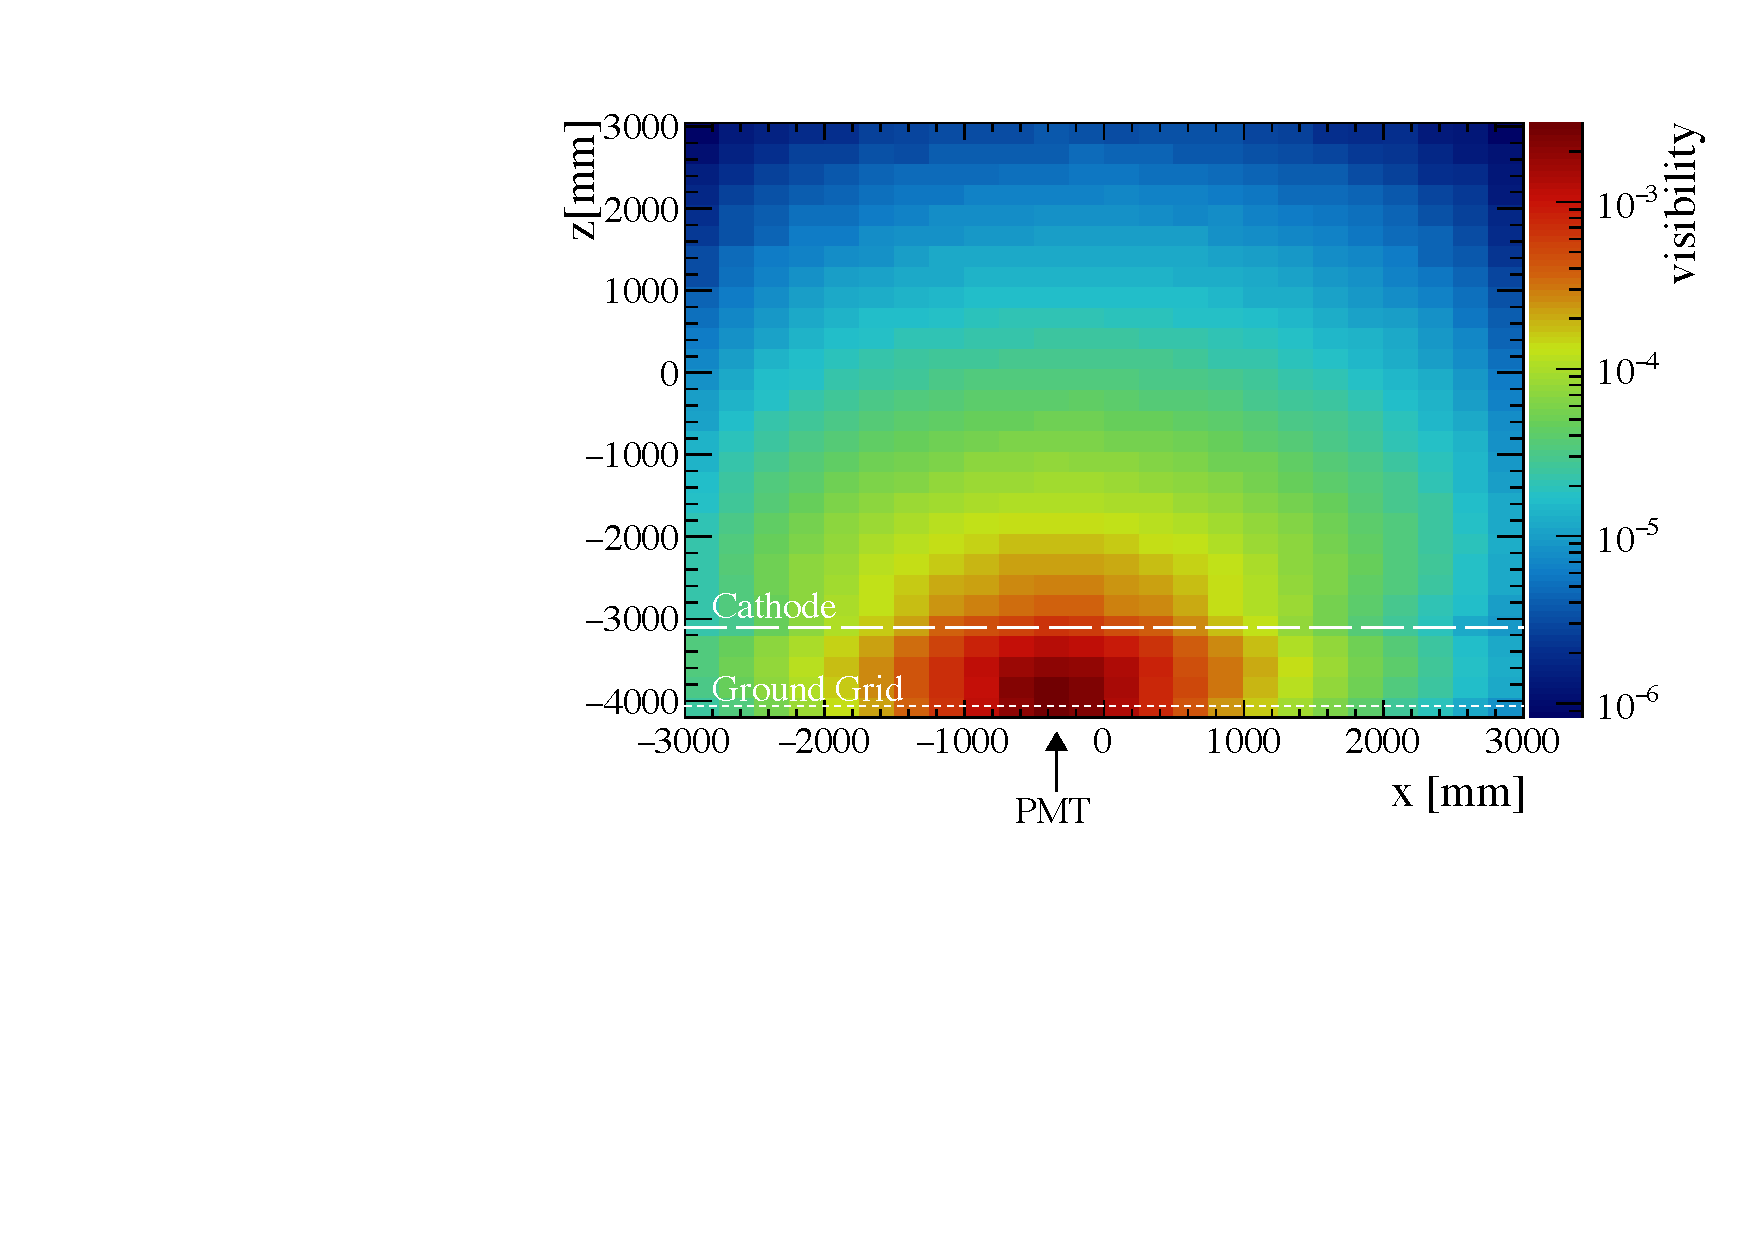
\includegraphics[width=0.45\textwidth]{dppd_6_1_1_c}
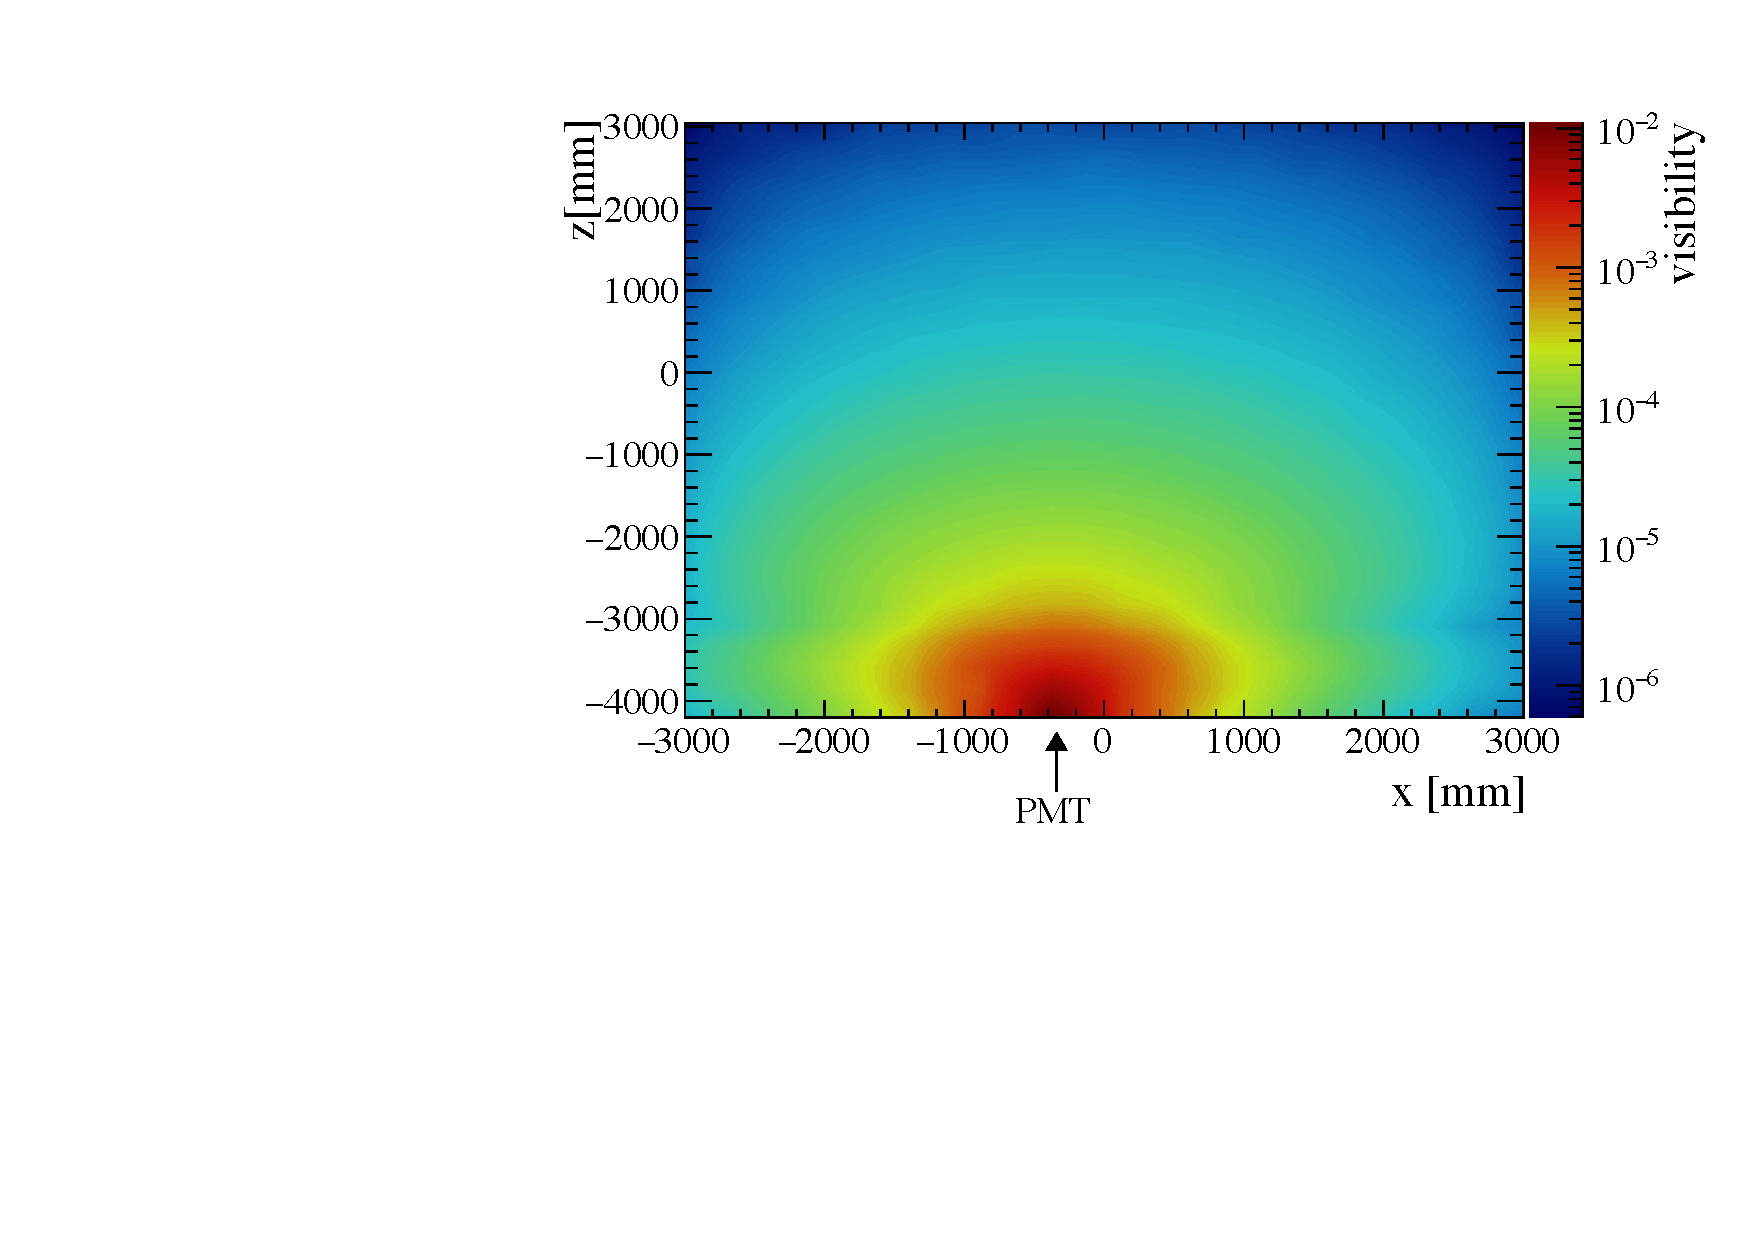
\includegraphics[width=0.45\textwidth]{dppd_6_1_1_d}
\end{dunefigure}

\subsubsection{Parametrization from the light maps}
\label{subsec:fddp-pd-6.1.2}

Without considering the border effects, where the photons are mostly absorbed, it is intuitive that the visibility and the time profile depend only on the source to \dword{pmt} distance.

This approach has been followed for the SBND~\cite{sbnd} light simulation and is considered for the \dword{dpmod} as well. In Figure~\ref{fig:dppd_6_1_2}, the evolution of the visibility and the peak time as a function of the source to \dword{pmt} distance are shown. As these plots have been generated from the light maps, where the borders are taken into account, the same evolutions are also presented only for voxels at least \SI{1}{m} away from the active volume boundaries. For the visibility, the structure is quite complicated when taking all the voxels highlighting the complexity of the light simulation in a closed space. When looking at voxels away from the boundaries, one can see a clear correlation between distance and visibility. As for the time distribution (here for the peak time, but same goes for $t_0$ and $\sigma$ parameters), one can notice two different regimes for short and large distance (the transition being at around \SI{2}{m}).

This preliminary study is quite encouraging for the light simulation in the FD module, at least for light sources being far away from the fiducial volume boundaries. As it is complicated to disentangle the effects due to the propagation and absorption parameters from the light maps, a careful dedicated study should be performed in order to get parametrization of the visibility and time distribution parameters as a function of the photon traveling distance.

\begin{dunefigure}[Evolution of the visibility and peak time as a function of the source-\dword{pmt} distance as simulated in the \dword{pddp} geometry (Preliminary study).]{fig:dppd_6_1_2}
{Evolution of the visibility (top) and peak time (bottom) as a function of the source-\dword{pmt} distance as simulated in the \dword{pddp} geometry (Preliminary study). On the left, all voxels are considered, on the right only the voxels at least 1\,m away from the fiducial border are considered.}
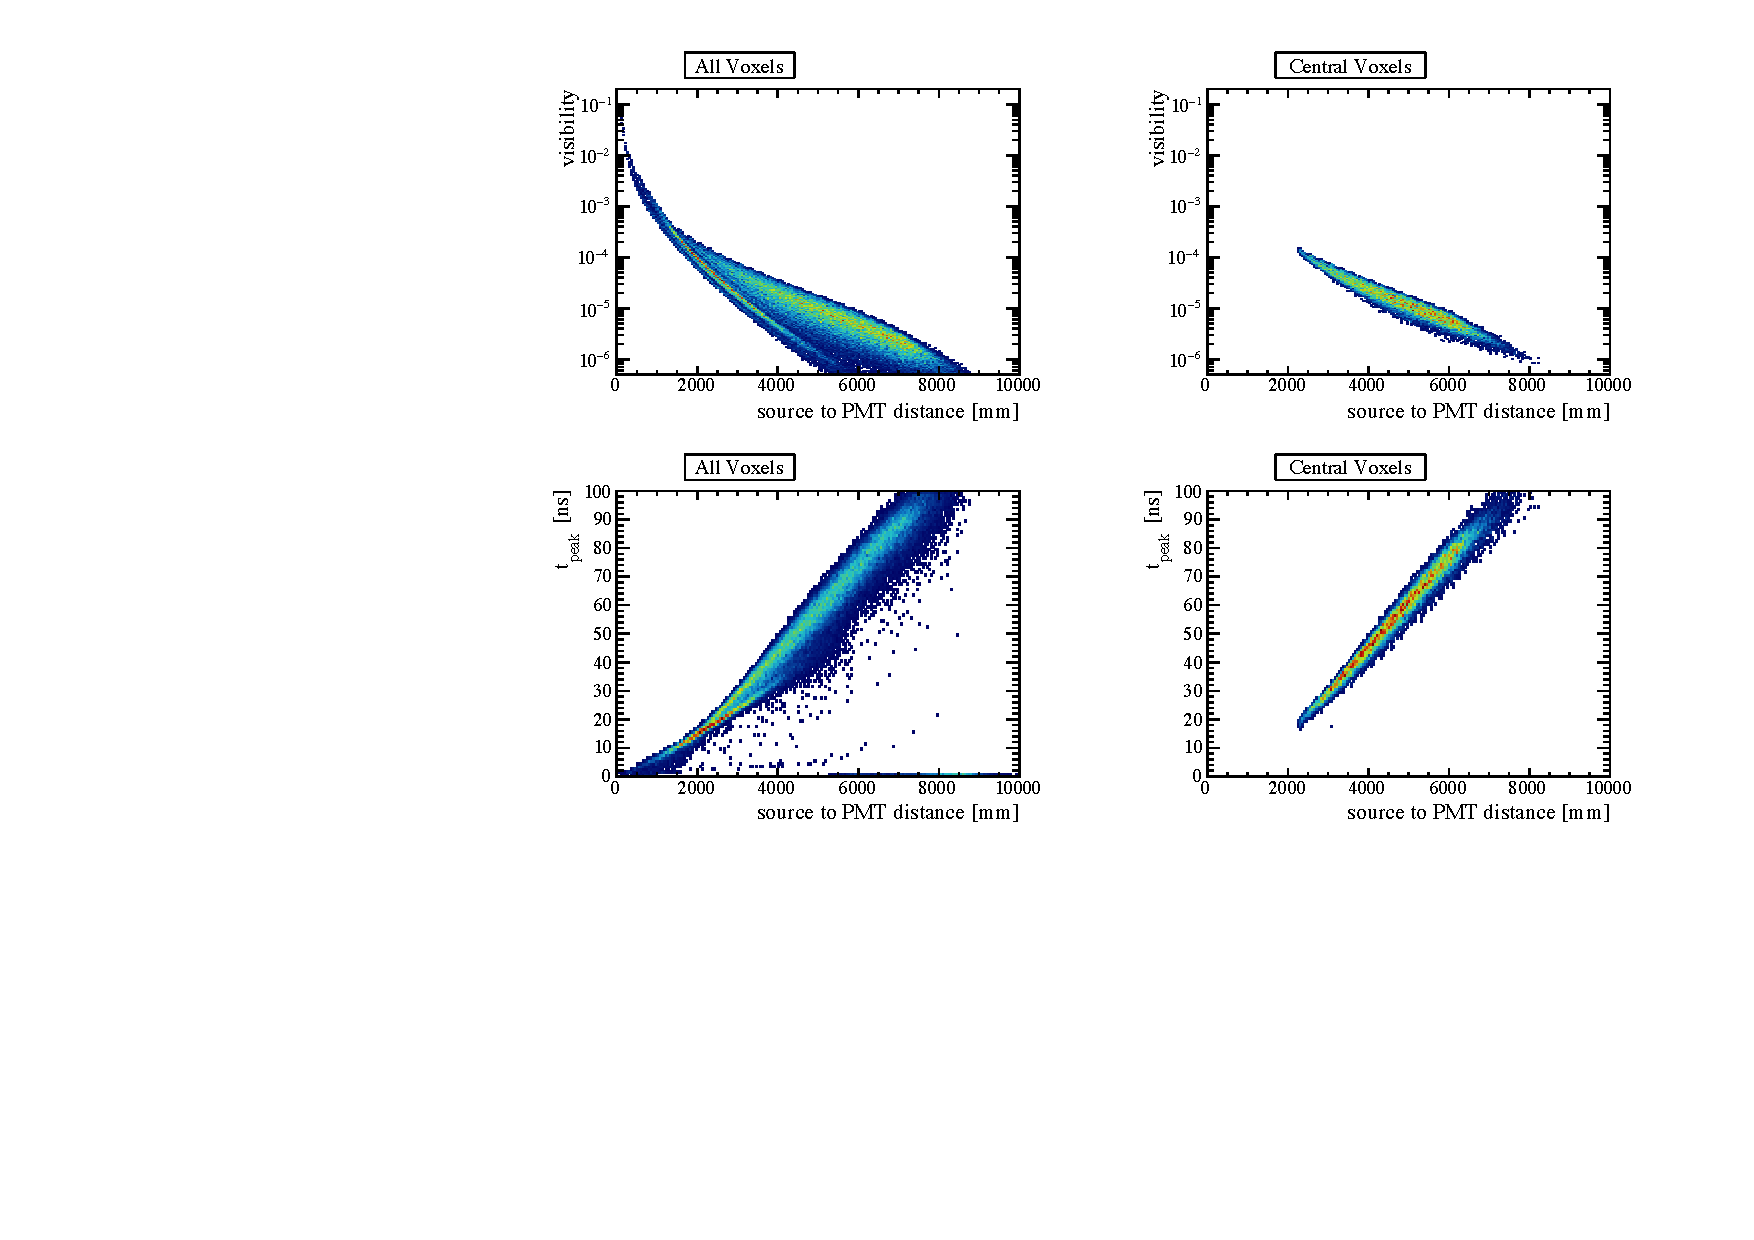
\includegraphics[width=0.75\textwidth]{dppd_6_1_2}
\end{dunefigure}

\subsubsection{Analytical approach}
\label{subsec:fddp-pd-6.1.3}

The propagation of light in a uniform material such as \lar can be described by the Fokker-Planck diffusion equation:

$$\frac{\partial}{\partial t}p(x,y,z,t) = D\left[\frac{\partial^2}{\partial x^2}p(x,y,z,t) + \frac{\partial^2}{\partial y^2}p(x,y,z,t) + \frac{\partial^2}{\partial z^2}p(x,y,z,t)\right]$$ 

where $D$ is the diffusion coefficient. In an unbound medium, the Fokker-Planck equation is solved by the Green function:

\begin{eqnarray*}
G(\textbf{r}, t; \textbf{r}_0, t_0) &=& \frac{1}{[4\pi D c (t-t_0)^{3/2}]}\exp\left(-\frac{|\textbf{r}-\textbf{r}_0|^2}{4Dc(t-t0)}\right) \\
D &=& \frac{1}{3(\mu_A + (1-g)\mu_S)}
\end{eqnarray*}

where $\mu_A$ and $\mu_S$ are the absorption and scattering coefficients respectively (both in units of m$^{-1}$), $g$ is the average scattering cosine ($g$ = \num{0.025}). In \lar with the default optical properties of Table \ref{tab:dppd_t_6_0}, $D$ = \SI{18.8}{\cm}. In a bound medium, with full absorption of the photons by the \dword{fc} and \dwords{lem}, a few additional techniques have to be used to obtain a solution. With this method, it takes only a few ms to have the photon density at a given \dword{pd} from a specific point source. From preliminary studies, a relatively good agreement between analytical approach and full simulation has been found. In particular, the arrival time distributions of photons on the \dwords{pmt} are well reproduced. The only drawback is that one cannot easily implement/study a complicated geometry including regions that are semi-transparent to light. Hence, the comparisons of the visibilities that one gets from the two methods are not in agreement in the overall light yield, but have a very similar trend in terms of spatial dependences. Some studies are ongoing in order to improve the analytical method results as this approach could be extremely powerful for physics studies in the FD module.

\subsubsection{Simulation of light yield}
\label{subsec:fddp-pd-6.1.4}
The light collected per \dword{pmt} can be simulated together with the charge for crossing tracks in a standard simulation code where a detailed description of the detector is not needed. At each step of the track propagation, the energy deposited is computed by Geant4. This energy is converted into number of electrons and photons produced. As for the light simulation, the number of photons reaching each \dword{pmt} and their time of arrival is now obtained from the light maps. As an example, the light yield from a uniform generation of \SI{10}{MeV} electrons in the active volume is shown in Figure \ref{fig:dppd_6_1_4}. The number of \phel{}s/MeV shown is summed over all \dwords{pmt} and average over the $y$ axis ($z$ being the drift direction). One can notice the large spread in terms of light yield.

\begin{dunefigure}[Light yield in terms of \phel/MeV summed over all \dwords{pmt} and averaged along the y-axis.]{fig:dppd_6_1_4}
{Light yield in terms of \phel/MeV summed over all \dwords{pmt} and averaged along the y-axis. The mean of all voxels gives a light yield of 2.5 \phel/MeV, although the distribution is not uniform, in particular along the z (drift) axis.}
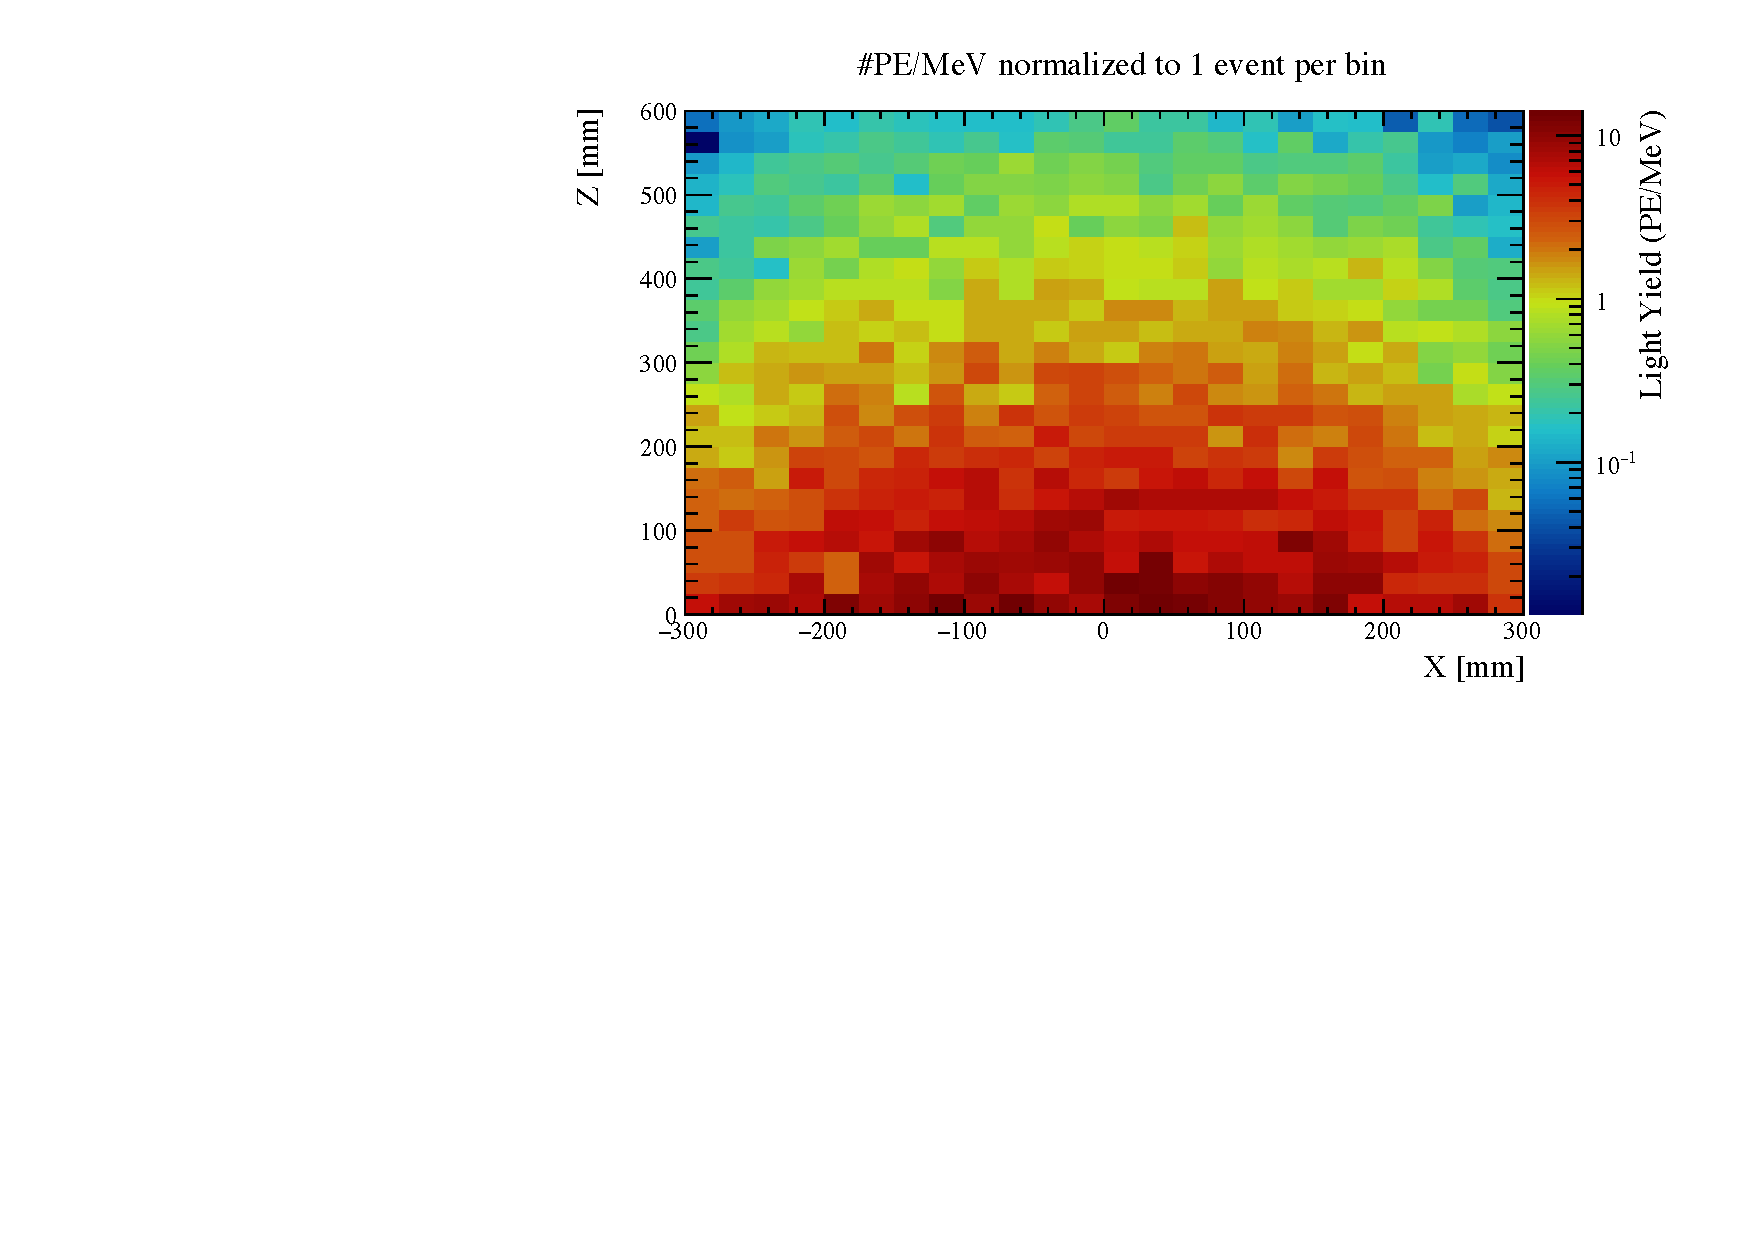
\includegraphics[width=0.6\textwidth]{dppd_6_1_4}
\end{dunefigure}

For larger volumes such as the DUNE FD, the light maps might be too big and the time spent accessing the four parameters might strongly reduce the speed of the simulation. Either the parametrization method or the analytical approach are foreseen to replace the current light map usage, the exact strategy is yet to be defined.

%%%%%%%%%%%%%%%%%%%%%%%%%%%%%%%%%
\subsection{Light data in DP prototypes}
\label{sec:fddp-pd-6.2}

The DP demonstrator ( \dword{wa105} $3\times1\times1$\,m$^3$) was operated from June to November 2017 with cosmic data. About \num{5} million light events were taken with various configurations. The study of the S1 light as a function of the drift field was performed. An example of an averaged waveform fitted to a fast and a slow scintillation components is shown in Figure~\ref{fig:dppd_6_2}. The amount of S2 light can be monitored as a function of the extraction and \dword{lem} amplification fields.

\begin{dunefigure}[Averaged waveform of the S1 light signal taken with one \dword{pmt} from the  \dword{wa105} $3\times1\times1$\,m$^3$ \lar DP TPC]{fig:dppd_6_2}
{Averaged waveform of the S1 light signal taken with one \dword{pmt} from the  \dword{wa105} $3\times1\times1$\,m$^3$ \lar DP TPC, fitted with a function (red line) that is the sum of a Gaussian, parametrized by t$_0$ and $\sigma$, and two exponential functions, with decay time constants $\tau_{fast}$ and $\tau_{slow}$, and normalization factors $A_{fast}$ and $A_{slow}$}
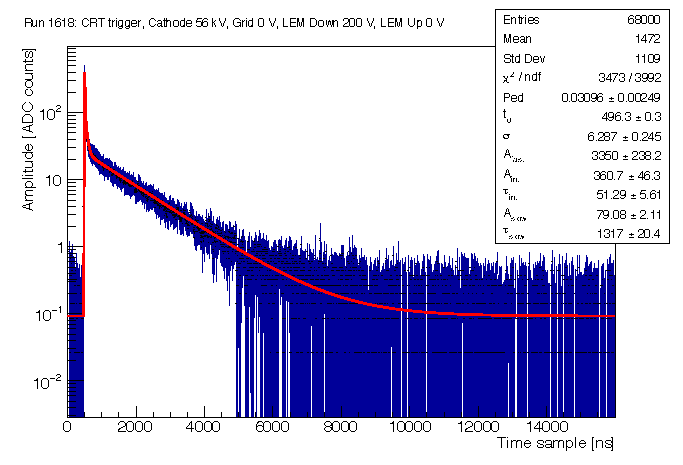
\includegraphics[width=0.6\textwidth]{dppd_6_2}
\end{dunefigure}

Light maps have also been generated with the demonstrator geometry, and data/MC comparisons are ongoing. The preliminary results look promising, although the statistics in each setting and the relatively small size of the detector still constitute a challenge to extract the entire optical properties of the \lar.


%%%%%%%%%%%%%%%%%%%%%%%%%%%%%%%%%
\subsection{Simulation of physics events}
\label{sec:fddp-pd-6.3}

A preliminary study to understand whether the \dual \dword{pd} technical design meets the experiment's physics requirements has been performed. In this study, event topologies of interest for DUNE physics have been simulated using \larsoft fast optical simulation tools.

The simulation framework used represents our current state-of-the-art. It includes realistic models for the primary scintillation production yields in \lar, for Rayleigh scattering in \lar, for detector optical properties (such as \dword{fc} reflectivity and cathode transparency), for the density of \dwords{pmt} underneath the cathode, and for the quantum efficiency of the \dword{tpb}-coated \dwords{pmt} (taken to be \num{20}\%). On the other hand, these simulations do not yet include the full \dword{dpmod} geometry, but are rather performed in a \dword{pddp} geometry with the same average \dword{pmt} density as the one proposed here for the \dword{dpmod} (one \dword{pmt} per m$^2$). Relevant aspects such as secondary scintillation light emission in gaseous argon (a nuisance for event $t_0$ determination), light absorption in \lar, electronics effects, reconstruction effects, and background contributions coming from $^{39}$Ar decays are not accounted for either in this study. While more realistic simulation results including the above effects will be produced on the DUNE TDR timescale, this preliminary study already provides a sense of the capabilities of the planned \dword{pd} design.

Figure~\ref{fig:dppd_6_3_1} shows the expected light yield for SN neutrino CC interactions. As a representative $\nu_e$ flux from a supernova neutrino burst, we assume a Fermi-Dirac distribution with $T$=\SI{3.5}{\MeV} temperature and no neutrino oscillation effects, yielding an average neutrino energy of about 11~MeV. Low-energy $\nu_e$ CC interactions throughout the entire \lartpc active volume are generated with the \larsoft-based Marley package. For the assumed SN neutrino flux and for a single interacting neutrino (hence, after convoluting flux and cross-section effects), Marley expects about \SI{19}{\MeV} of energy deposited in the \lar active volume, primarily from the final state electron and from nuclear de-excitation gamma rays. The left panel of Figure~\ref{fig:dppd_6_3_1} shows a broad light yield distribution, averaging at about \num{50} detected \phel{}s per interaction and after summing all \dwords{pmt}. This is as expected from the light yield distributions per deposited energy shown in Figure~\ref{fig:dppd_6_1_4}. The right panel shows the fraction of SN $\nu_e$ CC interactions within the \lartpc active volume above a given \phel detection threshold, as a function of the \phel threshold. From the figure, we conclude that about a 70\% fraction of SN $\nu_e$ CC interactions would be seen by the \dword{pd}, if the detector threshold was set at \num{10}~\phel{}s on the sum of the \dword{pmt} charges.

\begin{dunefigure}[Photon detector response for simulated SN neutrino interactions in the \dword{pddp} geometry.]{fig:dppd_6_3_1}
{Photon detector response for simulated SN neutrino interactions in the \dword{pddp} geometry. Left panel: distribution of detected \phel{}s per neutrino interaction, for SN $\nu_e$ CC interactions throughout the active volume. Right panel: fraction of SN $\nu_e$ CC interactions above \phel threshold, as a function of the \phel threshold.}
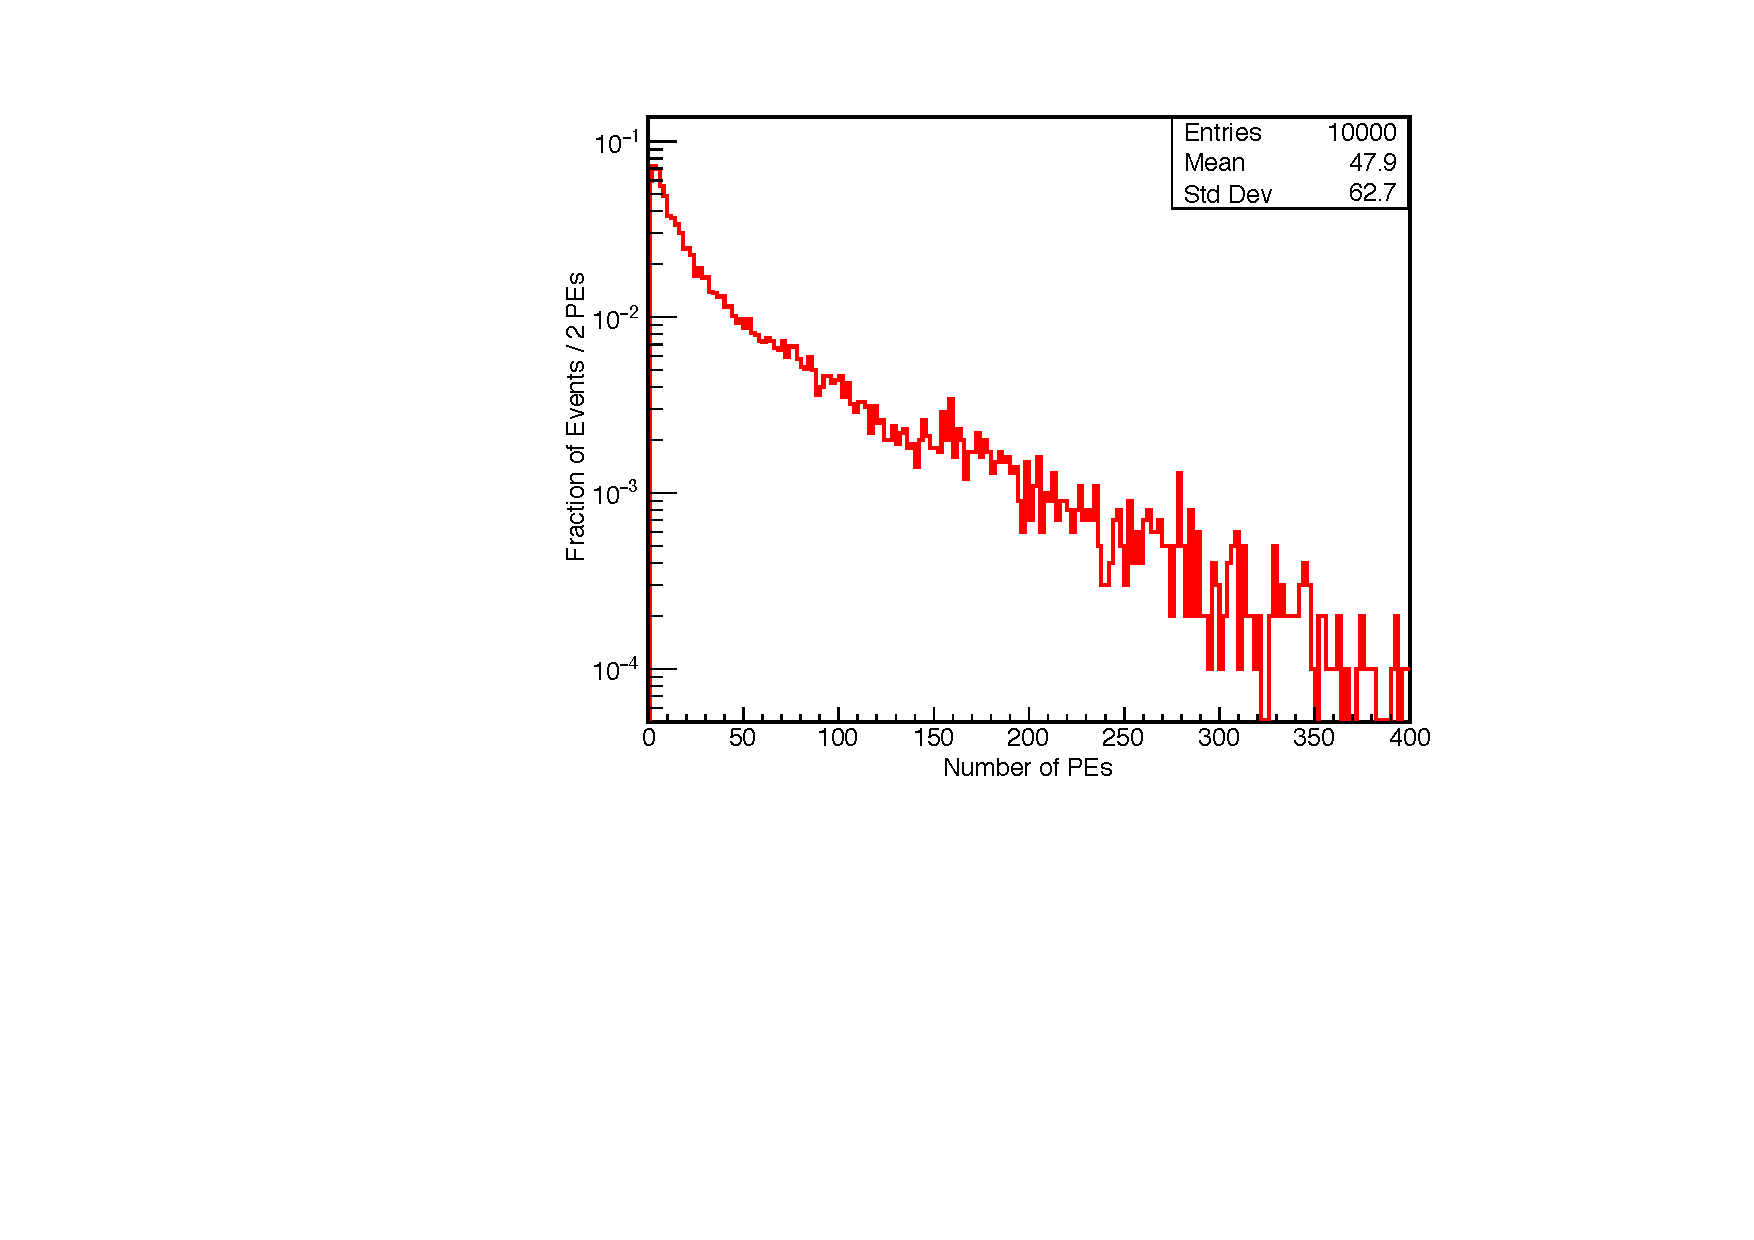
\includegraphics[width=0.44\textwidth]{dppd_6_3_1_1} \hfill 
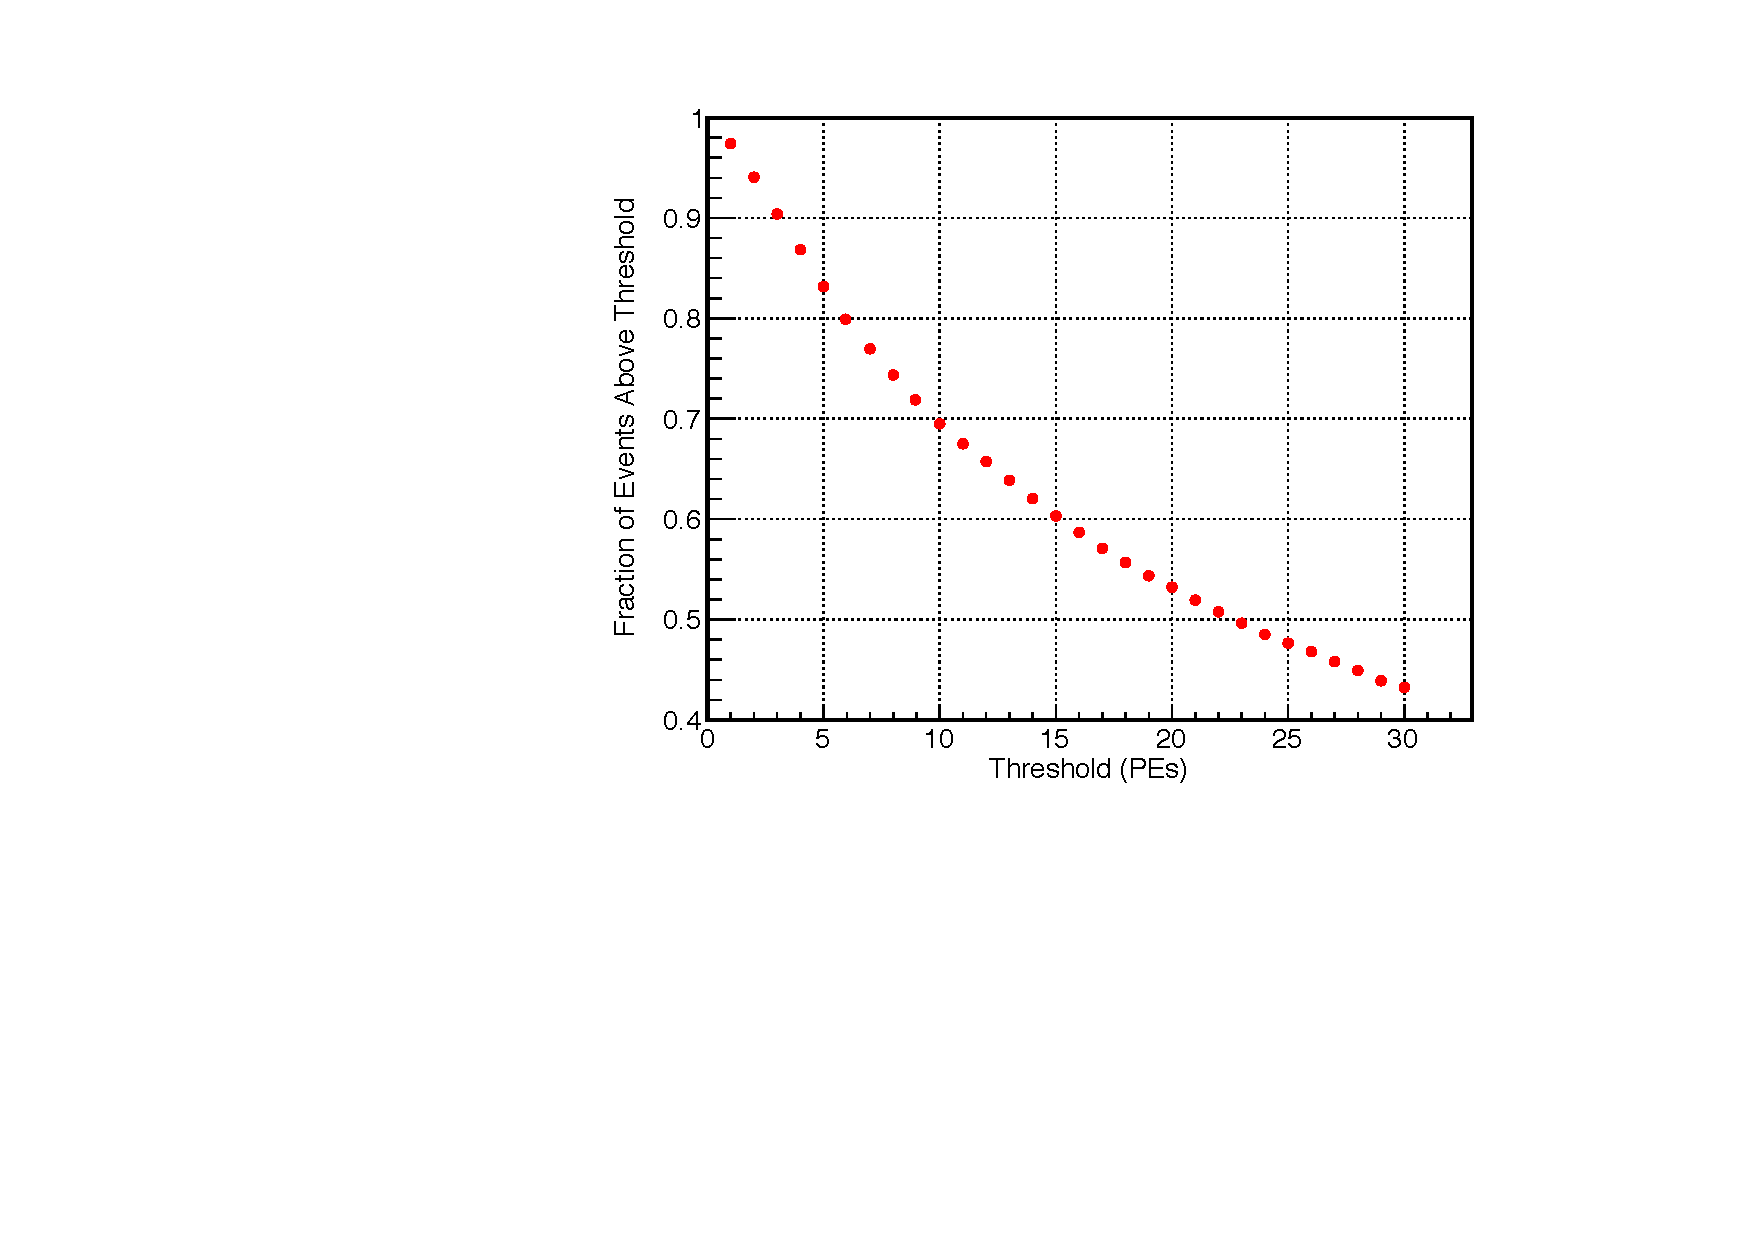
\includegraphics[width=0.44\textwidth]{dppd_6_3_1_2} 
\end{dunefigure}

Figure~\ref{fig:dppd_6_3_2} shows the corresponding plots for a representative nucleon decay final state in DUNE, namely $p\to\bar{\nu}K^+$. Nucleon decay events are generated using GENIE, accounting for both initial and final state nuclear effects in argon nuclei. Particles exiting the nucleus are then propagated in \lar using all relevant, Geant4-based, physics processes. The deposited energy per nucleon decay, of order \SI{300}{\MeV}, is much higher than the one per SN neutrino interaction. As a result, the expected light yield for $p\to\bar{\nu}K^+$ events throughout the active volume, shown in the left panel of Figure~\ref{fig:dppd_6_3_2}, averages to about 800~\phel{}s in this case. The right panel of Figure~\ref{fig:dppd_6_3_2} shows that about a 98\% fraction of $p\to\bar{\nu}K^+$ decays in the TPC active volume are expected to be seen by the \dword{pd}, for a \dword{pd} threshold of 10~\phel{}s on the \dword{pmt} charge sum.

\begin{dunefigure}[Photon detector response for simulated nucleon decays in the \dword{pddp} geometry.]{fig:dppd_6_3_2}
{Photon detector response for simulated nucleon decays in the \dword{pddp} geometry. Left panel: distribution of detected \phel{}s per nucleon decay, for $p\to\bar{\nu}K^+$ decays throughout the active volume. Right panel: fraction of $p\to\bar{\nu}K^+$ decays above \phel threshold, as a function of the \phel threshold.}
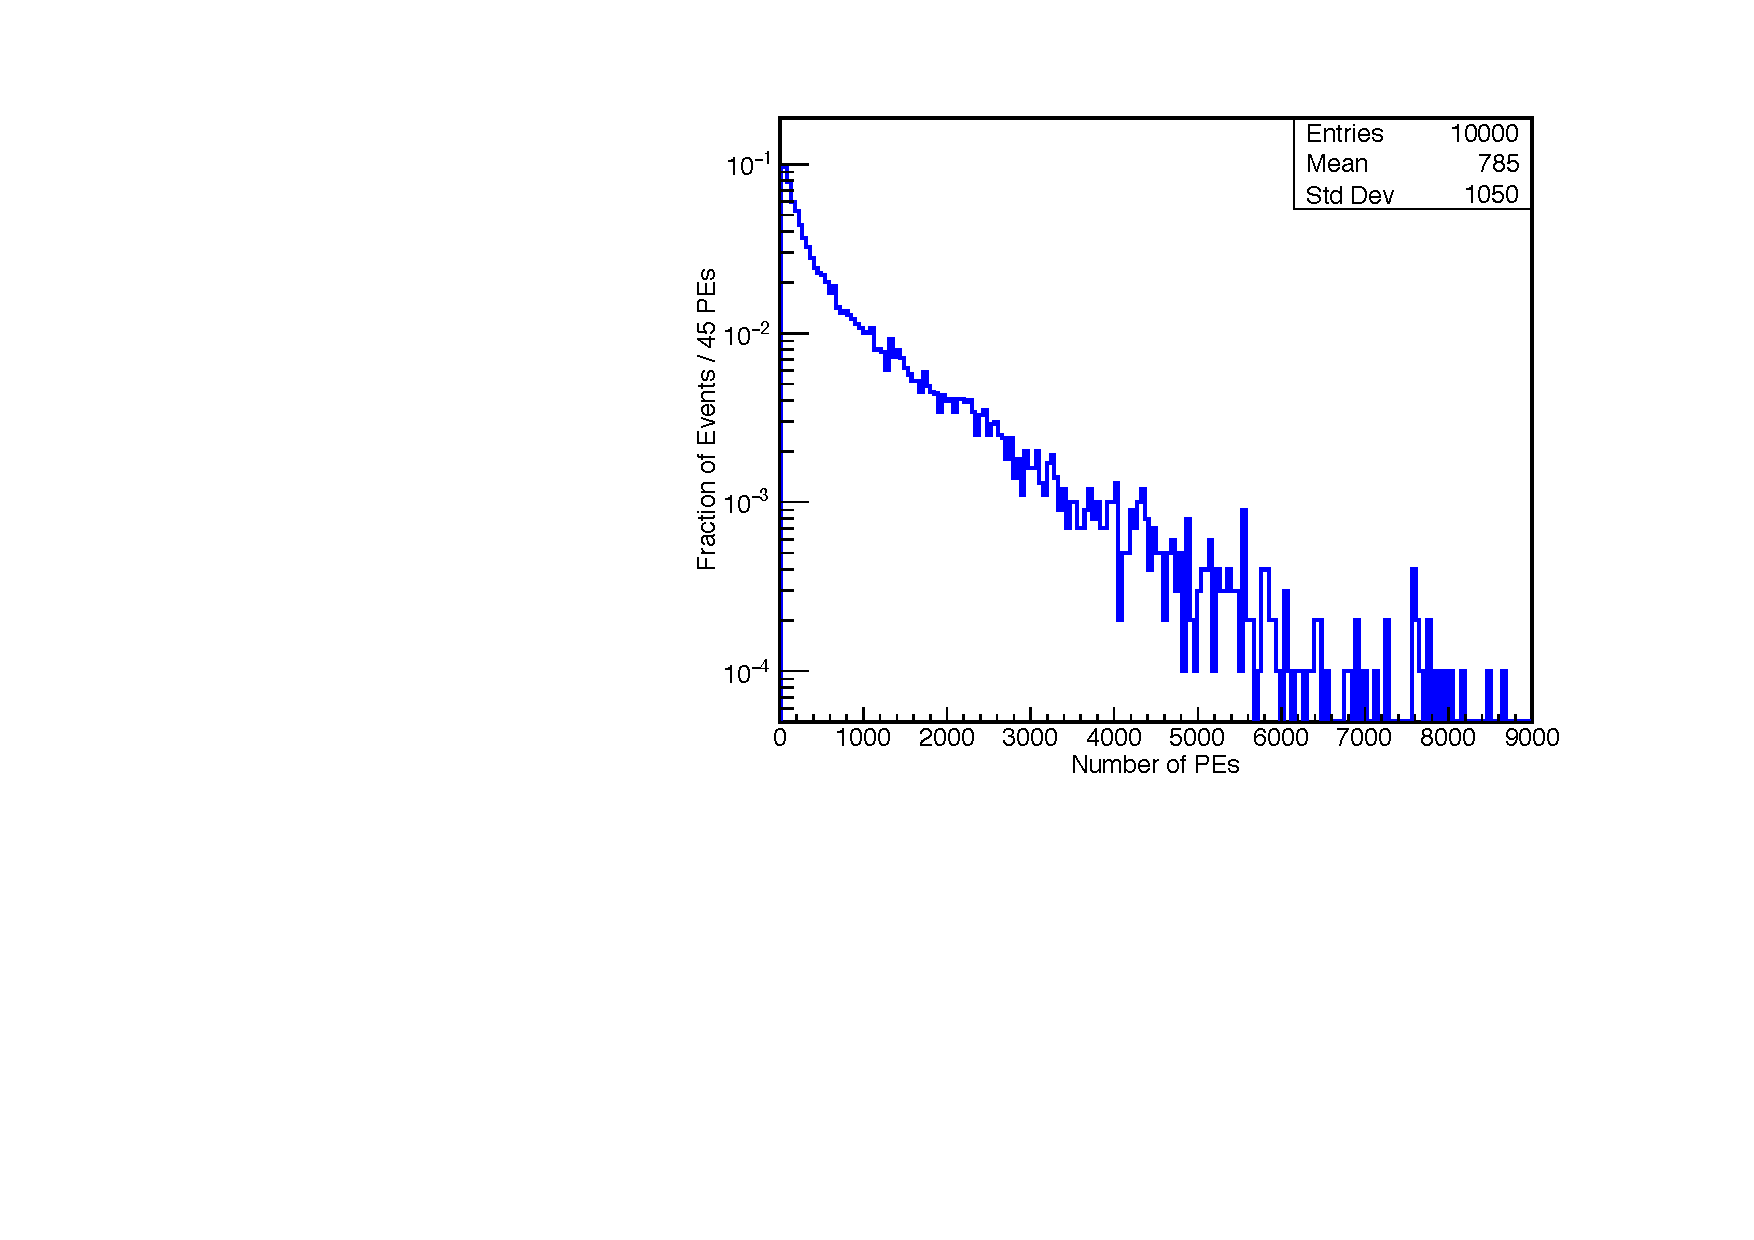
\includegraphics[width=0.44\textwidth]{dppd_6_3_2_1} \hfill 
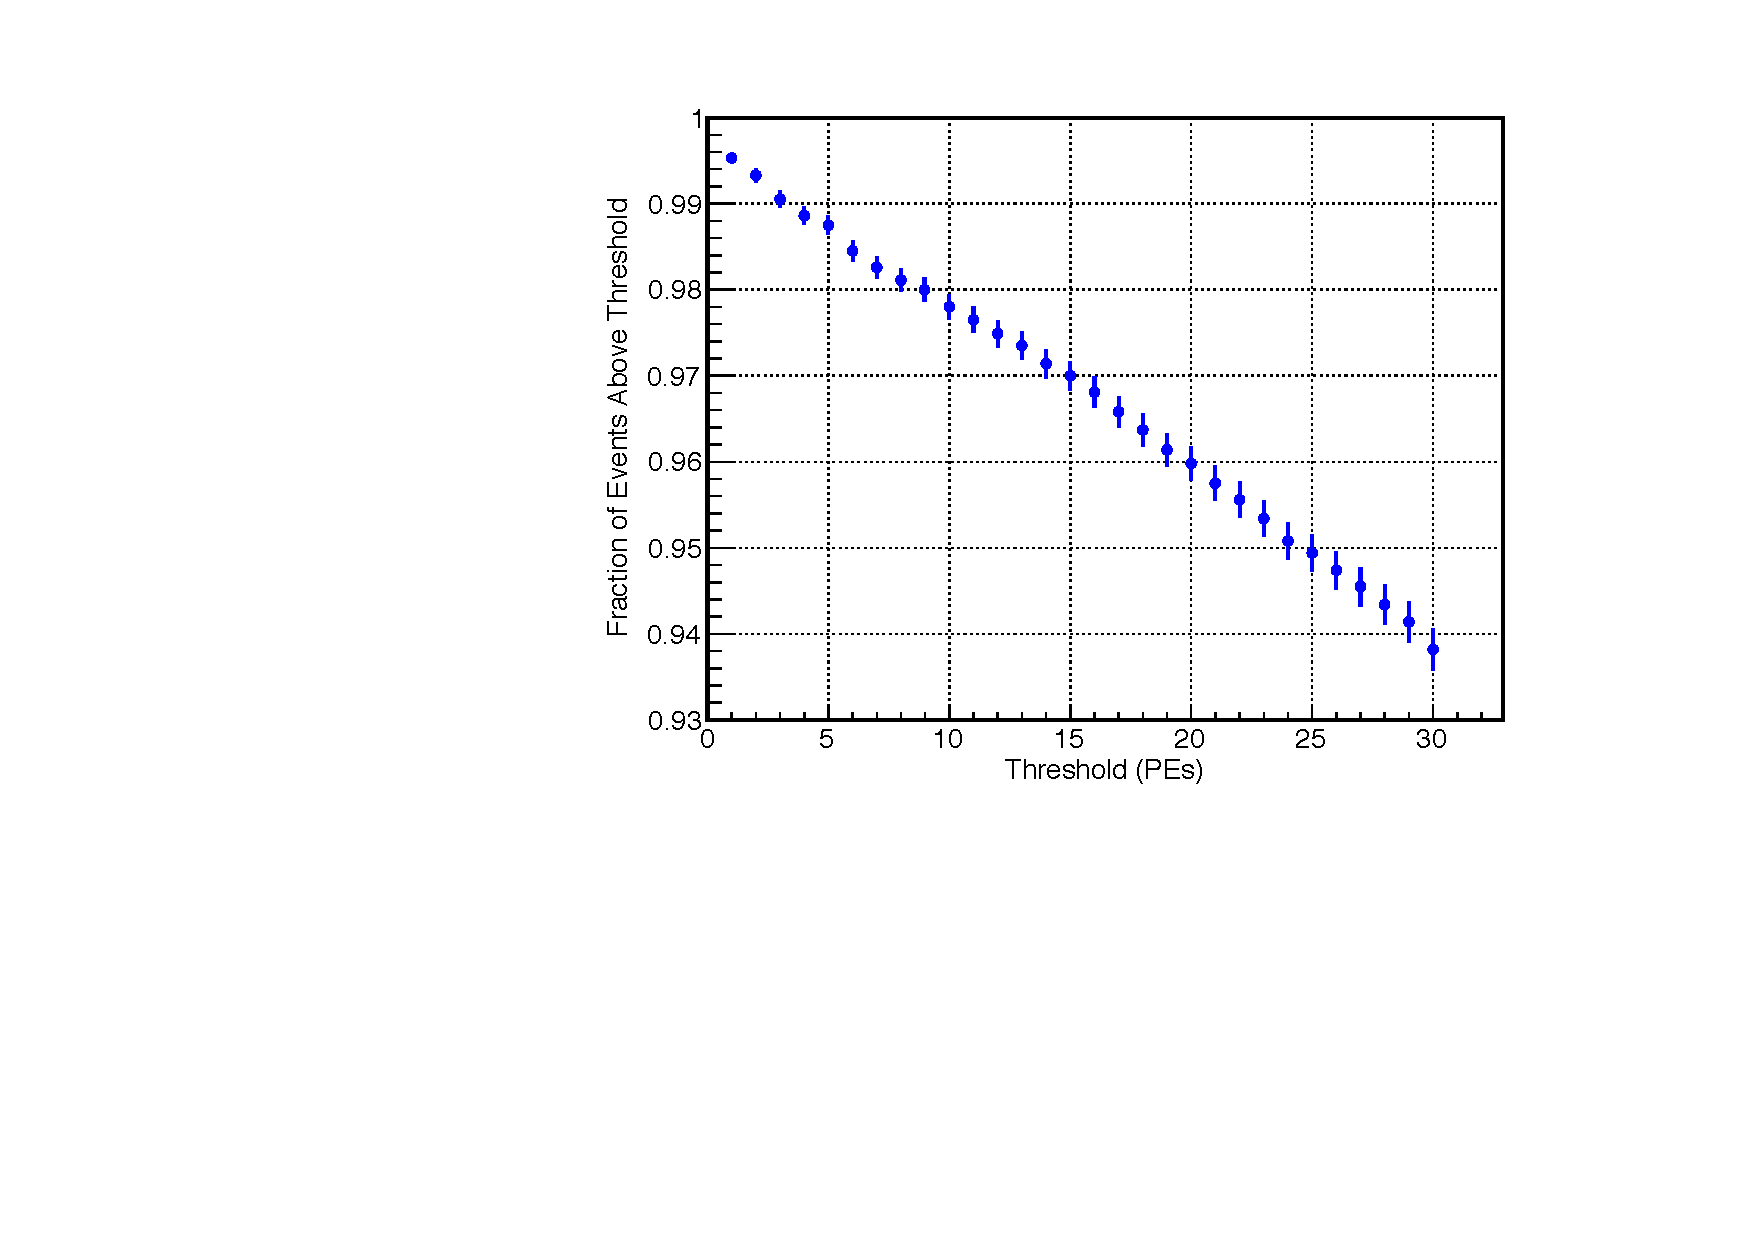
\includegraphics[width=0.45\textwidth]{dppd_6_3_2_2} 
\end{dunefigure}

%%%%%%%%%%%%%%%%%%%%%%%%%%%%%%%%%%%%%%%%%%%%%%%%%%%%%%%%%%%%%%%%%%%%
\section{Photon Detector Operations}
\label{sec:fddp-pd-7}

%%%%%%%%%%%%%%%%%%%%%%%%%%%%%%%%%
\subsection{Trigger Strategy}
\label{sec:fddp-pd-7.2}

As explained in section \ref{sec:fddp-pd-1.5}, the \dword{pds} will operate in different acquisition modes. These modes include the external trigger, which is the case of the beam events; the trigger for non-beam events such as  \dwords{snb}; and the calibration mode. 

In the \lartpc there are different uses of the light signal: cosmic ray/track timing for the reconstruction; non-beam events trigger such as SN neutrino burst, atmospheric neutrinos, and proton decay; and calorimetry, as the light and charge signal are anti-correlated. These physics studies imply different requirements in terms of dynamics of the electronics and data sampling, from a few \phel to a much higher level.

For the non-beam event trigger strategies, the requirements can be very different. In the event of a nearby (10\,kpc)  \dword{snb}, it is expected that a few thousands of neutrinos will homogeneously interact in the detector for a period as long as $\sim$\SI{100}{s}. Hence, the  \dword{snb} trigger strategy is mostly driven by the energy threshold set for $\nu$ detection and its efficiency: \SI{30}{MeV} is sufficient for a galactic SN, \SI{5}{MeV} is needed for a burst in Andromeda. A high-efficiency trigger for proton decay events has to be designed considering the worst case scenario, e.g. the event happening at the top of the detector, \SI{12}{m} away from the closest \dword{pmt}. In order to minimize the amount of spurious triggers, one can think of signal thresholds for a cluster of close-by \dwords{pmt}.

All these important studies will be further investigated once a reliable light simulation of the \dword{dpmod} is available. For the DP technology, the main light trigger concerns are the amount of light collectable for a photon traveling distance of \SI{12}{m} and the S1/S2 separation. The data that will be collected in the \dword{pddp} will provide crucial inputs for the optimization of the \dword{dpmod} light-collection system and for the design of an efficient trigger strategy for rare non-beam events. 

The \dword{pds} trigger will be flexible to fulfill the different physics requirements explained before. The light readout \dword{fe} board will be in charge of the \dword{pds} trigger generation. The trigger will be decided based on the coincidence of several \dword{pmt} signals over a threshold during a time window. The number of \dwords{pmt} that contribute to the trigger, the signal threshold and the length of the coincidence time window will be programmable on-line to be able to adapt to different physics cases.


%%%%%%%%%%%%%%%%%%%%%%%%%%%%%%%%%
\subsection{Data Quality Monitoring}
\label{sec:fddp-pd-7.3}

The \dwords{pmt} installed at the bottom of the tank will be operated for 10-20 years with no possibility to access them. Monitoring tools to ensure data quality of the \dword{pds} will have to be developed to catch any malfunctioning detector before data analysis. For instance, the amount of dark noise and the stability of the \dword{pmt} response will have to be monitored over time. For the gain evolution, either studies of standard candles, e.g. from Michel electrons or average collected light produced by cosmic tracks, or with the dedicated calibration system are considered.

Monitoring tasks were performed during the 6 months of operation of the  \dword{wa105} $3\times1\times1$\,m$^3$ with no dedicated light calibration system. This and the forthcoming operation of the \dword{pddp}, will again provide crucial input towards the \dword{pds} monitoring system in the FD module.

%%%%%%%%%%%%%%%%%%%%%%%%%%%%%%%%%%%%%%%%%%%%%%%%%%%%%%%%%%%%%%%%%%%%
\section{Interfaces}
\label{sec:fddp-pd-8}

The \dword{pds} will have several interfaces with other subsystems and the global DUNE systems. The interface documents related to DP \dword{pds} are given in Table~\ref{tab:dppd_t_8}. Only part of the basic interfaces are summarized below. 

\begin{dunetable}
[\dual \dword{pd} interface documents]
{|l|c| p{0.8\textwidth}}
{tab:dppd_t_8}
{\dual \dword{pd} interface documents}

\dual \dword{pd} Interface Document & DUNE docdb number \\ \toprowrule
DP Electronics & 6772 \\
DP \dword{hv} & 6799 \\
\dword{daq} & 6802 \\
Cryogenic Instrumentation and Slow Control & 6781 \\
DUNE Physics & 7087 \\
Software and Computing & 7114 \\
Calibration & 7060 \\
Integration and Testing Facility & 7033 \\
Detector and Facilities (LBNF) Infrastructure & 6979 \\
Installation & 7006 \\
\end{dunetable}


\begin{itemize}

\item DP Electronics: The \dword{pds} will share the same \dword{fe} electronics standard as the charge readout, which is $\mu$TCA based \cite{utca}. Specifications of both \dword{pds} and \dword{fe} electronics will be determined by the simulations and \dword{pddp} data.

\item \dword{hv}: This interface includes the consideration of the distance between the cathode and the \dword{pmt} planes, power dissipation from the \dwords{pmt} and the combined impact on the simulations.

\item \dword{daq}: The hardware interface will be mainly through optical fibers. DP \dword{pds} will be providing trigger and data in continuous streaming and the interface will also include the \dword{daq} software.

\item Cryogenic Instrumentation and Slow Control: The main interface points are the layout of the cryogenic instrumentation (e.g. purity monitors and light emitting system for the cameras) and the \dword{pmt} support structures and cabling; and the slow control and the \dword{pds} power supplies and calibration system.

\item DUNE Physics: \dual \dword{pd} will have interfaces with the overall physics requirements on energy and time together with classification of events, decay modes and neutrino flavors.

\item Software and Computing: This interface will be on the development of simulation, reconstruction and analysis tools.

\item Calibration: The DP \dword{pds} will participate in the Global Calibration Task Force and will provide handles to allow global monitoring of the \dword{pmt} performance.

\item Integration and Testing Facility: The operations at the Integration and Testing Facility are described in Section~\ref{sec:fddp-pd-9.2}. The interface items can be summarized as shipping and receiving of the DP \dword{pds} components and basic testing and repairing at the facility. The interface also includes recycling/returning the packaging materials.

\item Detector and Facilities (LBNF) Infrastructure: DP \dword{pds} will have \dword{pmt} mounting standing on the membrane, cold cables routed in cable trays to the ceiling \fdth flanges and racks, and cable trays on top of the cryostat. Other interfaces with the facility include access to conventional facilities and participation in the detector safety systems. 

\item Installation: This interface will be through the transportation of the DP \dword{pds} components to and between underground areas, clean room activities and storage, and installation coordination with the other teams. 

\end{itemize}

%%%%%%%%%%%%%%%%%%%%%%%%%%%%%%%%%%%%%%%%%%%%%%%%%%%%%%%%%%%%%%%%%%%%
\section{Installation, Integration and Commissioning}
\label{sec:fddp-pd-9}

%%%%%%%%%%%%%%%%%%%%%%%%%%%%%%%%%
\subsection{Transport/Handling}
\label{sec:fddp-pd-9.1}

The \dwords{pmt} of the \dword{pds} will be shipped from various locations following base and cable assembly for the \dword{tpb} coating at the Integration and Testing Facility. The shipping boxes will contain \num{24} \dwords{pmt} resulting in \num{30} total deliveries of \num{720} \dwords{pmt}. The \dwords{pmt} will be individually wrapped with different wrapping materials. The wrappings will have special openings to enable the basic electronics tests at the Integration and Testing Facility.

The \dwords{pmt} will be placed in modular shock absorbing assemblies inside the boxes. The assemblies will also allow a limited amount of safe inclination. The boxes will have integrated pellets for easy handling and short distance transportation. The \dwords{pmt} will reach the Integration and Testing Facility by means of air and ground transportation. Each box will have a dedicated bar-code which will be visible on each side. This bar-code will also be associated with the shipping documents. 

%%%%%%%%%%%%%%%%%%%%%%%%%%%%%%%%%
\subsection{Integration and Testing Facility Operations}
\label{sec:fddp-pd-9.2}

The \dword{pmt} boxes will be received by the Integration and Testing Facility (ITF). A shipping and delivery database will be managed by the ITF. The received status of the boxes will be available to the \dual \dword{pd} consortium as the boxes arrive at the ITF. The \dword{pds} characteristics database managed by the \dual \dword{pd} consortium will be updated accordingly to reflect the received status of the contents of the boxes. Each \dword{pmt} assembly will have identifying bar-codes that will be directly connected to the \dword{pds} characteristics database. This database will store the \dword{pmt} serial number, the base board serial number, special information about \dword{tpb} coating and assembly if any, and performance and calibration characteristics. This database will form the basis of the operations database providing the initial calibration values and it will also store information about the ITF tests and underground installation and commissioning tests.

The \dword{tpb} coating will be performed at the ITF in the coating stations. Then, the \dwords{pmt} will be placed back in their boxes, and dedicated testing electronics will be connected to the \dword{pmt} cables soldered to the \dword{pmt} bases. The test electronics will enable connecting several \dwords{pmt} at a time. The tests will include basic functionality checks of both the \dwords{pmt} and the base boards to assess the performance after transportation. No detailed performance characteristics will be measured at the ITF. The tests will be performed in a dedicated room with light and climate control. Once the performance of the \dwords{pmt} in a box is validated, the boxes will be closed with the original covers. Before closing, additional quality checks on the shock absorbing assemblies will be made.

The preparation of the \dword{pmt} boxes for underground transportation includes installing holding/lifting fixtures to the top and sides. The fixtures will allow crane operation. The boxes will be delivered to the surface station by ground transportation with relevant modification in the shipping database.

%%%%%%%%%%%%%%%%%%%%%%%%%%%%%%%%%
\subsection{Underground Installation and Integration}
\label{sec:fddp-pd-9.3}

Once the \dword{pmt} boxes are underground, the same top and side covers will be opened as at the ITF. The \dwords{pmt} will be carried to the underground storage area in sub-units of the shock absorbing assemblies which will be modular. The underground storage area for the \dword{pds} will be sufficiently large to store at least \num{30} \dwords{pmt} for continuous installation operations.

The removal of the individual \dword{pmt} wrappings will be done in the clean room. \dwords{pmt} together with their base boards will go through visual inspection by the \dword{pds} installation supervisor. Once signed-off, the installation can proceed with multiple \dwords{pmt} at a time by multiple teams. Cabling will be carried out in parallel and relevant database modifications will be made in-situ. The installation time management will be done in coordination with the cathode and \dword{fc} installation groups.

The bundles of cables will be routed through the cable trays along the cryostat walls from the \dword{pds} flanges. Following the mechanical mounting of the \dwords{pmt} to the cryostat floor, the \dword{pmt} cables will be 
connected to the cables coming from the flanges. In parallel, the calibration fibers will be installed and routed through cable trays.

%%%%%%%%%%%%%%%%%%%%%%%%%%%%%%%%%
\subsection{Commissioning}
\label{sec:fddp-pd-9.4}

The commissioning of the \dword{pds} will be performed in partitions. The size of the single partition will mainly be determined by the data acquisition system and the \dword{hv} system. The data acquisition system and \dword{hv} partitions will be commissioned, including the relevant control systems, prior to the connection of the \dwords{pmt} to these systems. Once the physical sector corresponding to a partition is installed, the \dwords{pmt} will be powered up and basic functionality and performance checks will be performed. These include pedestal data taking which consists of recording event data with external periodic triggering, and tests with the calibration system where the data taking is triggered in synchronization with a light source as described in Section \ref{sec:fddp-pd-5}.

As a result of the commissioning tests, the basic performance characteristics of the \dwords{pmt}, e.g. the dark count rate and gain, will be measured in their final places. Installation-related issues will be identified and eliminated at this stage. A commissioned sector will be the part of the overall detector and can join the global calibration data taking and commissioning.

%%%%%%%%%%%%%%%%%%%%%%%%%%%%%%%%%%%%%%%%%%%%%%%%%%%%%%%%%%%%%%%%%%%%
\section{Quality Control}
\label{sec:fddp-pd-10}


%%%%%%%%%%%%%%%%%%%%%%%%%%%%%%%%%
 \subsection{Production and Assembly}
 \label{sec:fddp-pd-10.1}
 
The quality control performed at the different institutions labs will include reception of \dwords{pmt} from the manufacturer and performing of the quality control tests to accept or return the \dwords{pmt} according to the acceptance/rejection criteria.

\begin{itemize}
\item The \dword{pmt} support structure design will be validated by immersing the \dword{pmt} mounted on it at cryogenic temperatures and at an over-pressure equivalent pressure of the 12\,m depth of \lar of the detector.
\item Design validation tests will be carried out in order to confirm that the \dword{pmt} base design fulfills the specifications at room and cryogenic temperatures. A cable with SHV connector will be soldered to each \dword{pmt} base to make easier the different base and \dword{pmt} tests and the final \dword{pmt} connection during the installation. The \dword{pmt} bases will be labeled (on the cable) in order to keep track of them. After production of the \dword{pmt} base boards they will be individually tested before mounting to the \dword{pmt} to verify that components are correctly mounted. Latter they will be cleaned and tested at maximum voltage on argon gas environment to confirm that there are no sparks on these (worst case) conditions.
After mounting the bases on the \dwords{pmt} they will be tested again in argon gas at maximum voltage to confirm that there are no sparks due to bad soldering.
\item All the light readout units (\dword{pmt} + base + support) will be tested and characterized in liquid nitrogen in order to check their performance at cryogenic temperature and to obtain a database with the most important parameters from each \dword{pmt} (gain vs voltage, dark counts, etc.). The \dword{pmt} base number attached to each \dword{pmt} will also be included on the database. 
\item The wrapping materials and techniques will be studied with one fully assembled light readout unit. The handling, transportation and installation scenarios will be carefully studied and the transportation box design will be validated. The transport box and \dword{pmt} wrapping must warrant darkness.
\item The light output of the  \dwords{led} and fibers light transmission from the photon calibration system will be measured with a power meter.
\end{itemize}

%%%%%%%%%%%%%%%%%%%%%%%%%%%%%%%%%
 \subsection{Post-Factory Installation}
 \label{sec:fddp-pd-10.2}
 
At the reception of the \dwords{pmt} at ITF (Integration \& Test Facility), they will go through verification measurements in order to discard possible damages during transportation. Gain vs voltage and dark current values will be compared with the ones obtained before transportation.

The \dword{tpb} coating will also be performed at the ITF. The first few samples will go through microscopic examination and surface uniformity tests, and the coating procedure will be validated. The production \dwords{pmt} will be randomly sampled for basic coating quality assurance.

After the transport from the ITF to the laboratory the \dwords{pmt} will be tested again before installation to confirm that there has not been any damage during the last transportation. During the installation, the \dwords{pmt} database will be updated with the position in the detector of each \dword{pmt} (identified by its serial number and base number). After installation, the full connection from the FE to the \dwords{pmt} will be checked. The FE channel and splitter number connected to each \dword{pmt} will, also, be included on the \dword{pmt} database. At the moment that it could be possible to make darkness in the detector the \dwords{pmt} will be tested applying voltage and checking the signal with a scope or with the FE electronics if they are already available.

%%%%%%%%%%%%%%%%%%%%%%%%%%%%%%%%%%%%%%%%%%%%%%%%%%%%%%%%%%%%%%%%%%%%
\section{Safety}
\label{sec:fddp-pd-11}

Safety is the highest priority at all stages of \dual \dword{pd} operations. Since DUNE is an international project, the international safety regulations will be followed closely during the course of preparation of safety documents.

Main risks at the production and testing sites are electrocution, exposure to excessive heat, chemicals and cryogenics, and heavy lifting. Detailed procedures will be developed by the relevant institutes and approved by the \dual \dword{pd} consortium. Contents of the electrical safety rules will range from utilizing regular power equipment to handling \dwords{pmt} for testing. The chemical and heat exposure hazards only concern the sites where the \dword{tpb} coating is going to be performed. The heavy objects that will carry safety risks will mainly be the \dword{pmt} delivery boxes.

The ITF \dual \dword{pd} safety regulations will be developed the same way. Main hazards on this site are electrocution and heavy lifting. Also, due to the density of shipments from all other subsystems, tripping and operations in limited space should also be considered.

The underground operation and installation safety rules will mainly follow the general facility rules on e.g. working in confined spaces, oxygen deficiency hazard and emergency procedures. \dual \dword{pd} specific safety rules will particularly be related to lifting of heavy objects for installation and working at heights for cabling.

%%%%%%%%%%%%%%%%%%%%%%%%%%%%%%%%%%%%%%%%%%%%%%%%%%%%%%%%%%%%%%%%%%%%
\section{Management and Organization}
\label{sec:fddp-pd-12}

The \dual \dword{pd} consortium was formed in 2017 and it is composed by eleven institutes from France, Peru, Spain, UK and USA. The charge of the \dual \dword{pd} onsortium is to plan and execute the construction, installation and commissioning of the DUNE DP FD \dword{pds}.


%%%%%%%%%%%%%%%%%%%%%%%%%%%%%%%%%
\subsection{Consortium Organization}
\label{sec:fddp-pd-12.1}

The \dual \dword{pd} consortium Leader (CL) is In\'{e}s Gil-Botella from CIEMAT (Spain) and the Technical Lead (TL) is Dominique Duchesneau from LAPP (France). They are members of the DUNE Technical Board and they represent the consortium to the overall DUNE collaboration. The CL is responsible for the subsystem deliverables and for the effective management of the consortium. The TL acts as the overall project manager and he is the interface to the International Project Office (IPO), and is responsible for monitoring/reporting progress against the agreed schedule and issues related to interface documentation.

The institutions participating in the consortium are responsible for the design or construction of a particular sub-system. It is hoped that the national groups within the consortia will be able to approach relevant funding agencies with a specific construction-phase proposal, such that a likely funding line can be established in or before 2019. The \dual \dword{pd} consortium is open to any new institution willing to join the current effort.

The current institutions participating in the \dual \dword{pd} consortium are summarized in Table \ref{tab:dppd_t_12_1}.

\begin{dunetable}
[\dual \dword{pd} consortium institutions]
{|l|l|l| p{0.8\textwidth}}
{tab:dppd_t_12_1}
{\dual \dword{pd} consortium institutions}

Country & Institution & Contact \\ \toprowrule
France & LAPP & Dominique Duchesneau \\
Peru & PUCP & Alberto Gago \\
Spain & IFAE & Thorsten Lux \\
Spain & CIEMAT & In\'{e}s Gil-Botella\\
Spain & IFIC & Michel Sorel \\
United Kingdom & University College London & Anna Holin \\
USA & Argonne National Lab & Zelimir Djurcic \\
USA & Duke University & Kate Scholberg \\
USA & University of Iowa & Jane Nachtman \\
USA & South Dakota School of Mines and Technology & Juergen Reichenbacher\\
USA & University of Texas at Austin & Karol Lang \\
% \colhline
\end{dunetable}

The \dual \dword{pd} consortium is divided in four working groups: photosensors and electronics, calibration system, mechanics and integration, and simulation and physics. The corresponding WG conveners are:
\begin{itemize}

\item WG1: Photosensors and Electronics - A. Verdugo (CIEMAT)
\item WG2: Calibration System - C. Cuesta (CIEMAT)
\item WG3: Mechanics and Integration - B. Bilki (Iowa)
\item WG4: Sim. \& Phys. - K. Scholberg (Duke), M. Sorel (IFIC), L. Zambelli (LAPP)

\end{itemize}

The \dual \dword{pd} consortium has regular bi-weekly meetings on Thursdays (4pm CET, 9am CST). Agendas and presentations can be found at: https://indico.fnal.gov/category/699/

%%%%%%%%%%%%%%%%%%%%%%%%%%%%%%%%%
\subsection{Planning Assumptions}
\label{sec:fddp-pd-12.2}

The optimization and final design of the \dual \dword{pd} system will be driven by:
\begin{enumerate}
\item \dword{pddp} data (expected by beginning of 2019)
\item Simulation studies (in progress)
\end{enumerate}

\dword{pddp} operation and data analysis are fundamental steps to understand if the current photon detection system considered as baseline, based on cryogenic \dwords{pmt} with \dword{tpb} coating, is able to provide $t_0$ for non-beam events, background rejection and triggering on non-beam events. These data will be used to tune the MC simulations and extrapolate the performance of the system to the DUNE Far Detector. 

Simulations are needed to determine and optimize the \dual \dword{pd} system to meet the physics requirements in terms of:
\begin{itemize}
\item Light collection efficiency
\item Number of channels
\item Photosensor requirements
\item Dynamic range of readout electronics and timing resolution
\item Trigger strategy on non-beam events
\end{itemize}

The DUNE physics requirements in terms of expected performance of the \dword{pds} should be provided by the DUNE Physics WG. Alternative design aspects of the proposed \dword{pds} considered as baseline for the \dword{dpmod} (see CDR document arXiv:1601.02984) will be developed based on the compatibility of \dword{pddp} data and MC light simulation results with the DUNE physics requirements.

%%%%%%%%%%%%%%%%%%%%%%%%%%%%%%%%%
\subsection{WBS and Responsibilities}
\label{sec:fddp-pd-12.3}

The \dual \dword{pd} consortium has developed a detailed breakdown of deliverables/responsibilities included in the overall DUNE collaboration Work Breakdown Structure (WBS), DUNE-doc-5594, coordinated by the IPO. The main deliverables are based on the \dword{pddp} photon detection system and are divided in seven topics: 

\textbf{WBS Element} \textit{- Institutions} \\
DP Photon Detection  System (\dual \dword{pds})
\begin{enumerate}
\item Management \dual \dword{pds} (includes milestones \& review dates) \textit{- LAPP, CIEMAT }
\item Physics \& Simulations \textit{- Duke, LAPP, IFIC, SDSMT, CIEMAT, PUCP, UCL, Texas-Austin}
\item Design, Engineering, R\&D and validation tests \textit{- Iowa, CIEMAT, IFIC, UCL, Texas-Austin, IFAE, SDSMT}
\item Production Setup (includes tooling) \textit{- UCL}
\item Production (includes component production, assembly, testing, \& QC) \textit{- Iowa, CIEMAT, IFAE, IFIC, UCL, Texas-Austin, Duke, SDSMT, LAPP}
\item Integration (contributions to activities at global integration facility) \textit{- SDSMT}
\item Installation (contributions to activities at SURF) \textit{- CIEMAT, IFIC, SDSMT, Iowa}
\end{enumerate}


%%%%%%%%%%%%%%%%%%%%%%%%%%%%%%%%%
\subsection{High-Level Cost and Schedule}
\label{sec:fddp-pd-12.4}

The cost of the baseline \dual  \dword{pds} will be defined in a separated document.

The main activities to be developed by the \dual \dword{pd} consortium during the next 16 months are focused to complete the Technical Design Report of the \dual \dword{pds}. The main high-level milestones are detailed in Table \ref{tab:dppd_t_12_4}

% Anne added newstyle table along with updates to dune.cls that are required to go with it
\begin{table}[htpb] \label{tab:dppd_t_12_4}
\scriptsize
\begin{center}
\caption{\dual \dword{pd} schedule of activities and milestones.}
\begin{tabular}{|l|c|c|c|c|c|c|}
\hline
\rowtitlestyle &  \multicolumn{4}{c|}{2018} & \multicolumn{2}{|c|}{2019} \\ % \hline
\rowtitlestyle {\bf Simulation \& Physics} & Q1 & Q2 & Q3 & Q4 & Q1 & Q2\\
\hline

Understanding the DUNE physics requirements affecting the \dual \dword{pd} system & & \cellcolor{gray} & & & & \\ \hline
Finalize the implementation of \dual optical simulation in \larsoft for \dword{pddp} & &  \cellcolor{gray} & & & & \\ \hline
Propose a solution for a full \dword{dpmod} optical simulation in \larsoft & & &  \cellcolor{gray} & & & \\ \hline
Include electronics response simulation & & &  \cellcolor{gray} & & & \\ \hline
Study the physics reach with the current \dual \dword{pd} performance and identify possible issues & & & &  \cellcolor{gray} & & \\ \hline
Tuning light simulation using \dword{pddp} light data & & & & &  \cellcolor{gray} & \\ \hline
Optimization of the \dual \dword{pd} performance to fulfil the physics requirements & & & & & &  \cellcolor{gray} \\ \hline
Definition of a trigger strategy & & & & & &  \cellcolor{gray} \\ \hline
\rowcolor{dunetablecolor}  \multicolumn{7}{|l|}{\bf Photosensors} \\
\hline
Review \dword{pmt} specifications \& readout electronics based on \dword{pddp} design & &  \cellcolor{gray} & & & & \\ \hline
Characterization \& certification plans \& test facility design & & &  \cellcolor{gray} & & & \\ \hline
Validation of \dwords{pmt} \& readout electronics performance with \dword{pddp} data & & & & &  \cellcolor{gray} & \\ \hline
Selection of \dword{pmt} \& wavelength-shifting & & & & &  \cellcolor{gray} & \\ \hline
Final design of voltage divider and \dword{hv}/signal splitters & & & & &  \cellcolor{gray} & \\ \hline
Final definition of readout electronics requirements & & & & &  \cellcolor{gray} & \\ \hline
\rowcolor{dunetablecolor} \multicolumn{7}{|l|}{\bf \dword{pmt} calibration system} \\ \hline
Initial design of the system for Technical Proposal & &  \cellcolor{gray} & & & & \\ \hline
Definition of calibration requirements & & &  \cellcolor{gray} & & & \\ \hline
Review the proposed design in light of \dword{pddp} calibration data & & & &  \cellcolor{gray} & & \\ \hline
Selection of components, production and testing plan & & & &  \cellcolor{gray} & & \\ \hline
\rowcolor{dunetablecolor} \multicolumn{7}{|l|}{\bf Mechanics} \\ \hline
Design of \dword{pmt} mechanical support \& production plans & &  \cellcolor{gray} & & & & \\ \hline
\dword{pmt} layout definition & & &  \cellcolor{gray} & & & \\ \hline
Review the proposed design in light of \dword{pddp} operation & & & & &  \cellcolor{gray} & \\ \hline
Definition of the mechanical integration with cryostat & & & & & &  \cellcolor{gray} \\ \hline
\rowcolor{dunetablecolor} \multicolumn{7}{|l|}{\bf Cabling \& flanges} \\ \hline
Definition of warm and cold cables & &  \cellcolor{gray} & & & & \\ \hline
Routing plan & & & & &  \cellcolor{gray} & \\ \hline
Flanges design & & & & &  \cellcolor{gray} & \\ \hline
\rowcolor{dunetablecolor} \multicolumn{7}{|l|}{\bf Quality Control} \\ \hline
QC plan and database definition & &  \cellcolor{gray} & & & & \\ \hline
\rowcolor{dunetablecolor} \multicolumn{7}{|l|}{\bf Interfaces} \\ \hline
Identification of hardware interfaces &  \cellcolor{gray} & & & & & \\ \hline
Identification of software interfaces & &  \cellcolor{gray} & & & & \\ \hline
\rowcolor{dunetablecolor} \multicolumn{7}{|l|}{\bf Integration, installation \& commissioning} \\ \hline
Transportation plan & &  \cellcolor{gray} & & & & \\ \hline
Safety requirements & & &  \cellcolor{gray} & & & \\ \hline
Integration facility design and definition of tests & & &  \cellcolor{gray} & & & \\ \hline
Underground installation plan & & & &  \cellcolor{gray} & & \\ \hline
Detector operation definitions and commissioning plan  & & & &  \cellcolor{gray} & & \\ \hline
\rowcolor{dunetablecolor} \multicolumn{7}{|l|}{\bf Management \& Organization} \\ \hline
Definition of milestones \& activities &  \cellcolor{gray} & & & & & \\ \hline
Initial schedule \& risks evaluation & &  \cellcolor{gray} & & & & \\ \hline
\dual \dword{pd} Technical proposal & &  \cellcolor{gray} & & & & \\ \hline
Initial WBS \& high-level cost estimations & &  \cellcolor{gray} & & & & \\ \hline
Identification of risks & & & & &  \cellcolor{gray} & \\ \hline
\dual \dword{pd} Technical Design Report & & & & & &  \cellcolor{gray} \\ \hline
WBS and institutional responsibilities \& cost & & & & & &  \cellcolor{gray} \\ \hline
\end{tabular}
\label{tab:schedule}
\end{center}
\end{table}
